\documentclass[12pt,a4paper]{article}
\usepackage[utf8]{inputenc}
\usepackage[T1]{fontenc}
\usepackage[polish]{babel}
\usepackage{geometry}
\usepackage{graphicx}
\usepackage{booktabs}
\usepackage{tabularx}
\usepackage{array}
\usepackage{float}
\usepackage{caption}
\usepackage{amsmath}
\usepackage{hyperref}
\geometry{margin=2cm}
\graphicspath{{dane/}}
\setlength{\parindent}{0pt}
\setlength{\parskip}{4pt}
\renewcommand{\arraystretch}{1.15}

\begin{document}
\begin{titlepage}
\noindent
\begin{tabularx}{\textwidth}{|>{\raggedright\arraybackslash}p{0.29\textwidth}|>{\raggedright\arraybackslash}X|>{\raggedright\arraybackslash}p{0.19\textwidth}|}
\hline
\textbf{grupa 6} & \textbf{10.11.2026} & \textbf{18.11.2026} \\[8mm]
\hline
\textbf{1. Ethernet} & \multicolumn{2}{l|}{} \\[6mm]
\hline
\textbf{Filip Będkowski, Danylo Drygo} & & \textbf{} \\[8mm]
\hline
\end{tabularx}
\vfill
\begin{center}
{\Huge \textbf{SPRAWOZDANIE}\\[5mm]
\Large Ethernet}
\end{center}
\vfill
\end{titlepage}
\newpage

\section{Cel ćwiczenia}
Celem ćwiczenia było poznanie technologii Ethernet oraz praktyczne sprawdzenie okablowania metalowego w standardzie RJ45. Podczas zajęć wykonywaliśmy następujące czynności:
\begin{itemize}
  \item identyfikację i pomiar kabli przyjętych do testów,
  \item przygotowanie końcówek typu RJ45 według standardów EIA/TIA 568A i 568B,
  \item testowanie kabli i ścieżek testera,
  \item testowanie okablowania z wykorzystaniem patchpanelu,
  \item identyfikację przyczyn usterek,
  \item kwalifikację okablowania przy użyciu Fluke CableIQ oraz porównanie jej z pomiarami testera podstawowego.
\end{itemize}

\section{Wstęp teoretyczny}
\subsection{Ethernet i adres MAC}
Ethernet jest rodziną standardów IEEE 802.3 przeznaczonych do budowy sieci lokalnych. Umożliwia on przesyłanie ramek pomiędzy kartami sieciowymi po wspólnym medium. Tradycyjny Ethernet opierał się na metodzie CSMA/CD, natomiast nowoczesne sieci Ethernet pracujące na przełącznikach korzystają głównie z pełnego dupleksu i nie wymagają wykrywania kolizji.

Adres MAC ma długość 48 bitów i jest zapisywany jako sześć bajtów szesnastkowo. Pierwsze 24 bity identyfikują producenta (OUI), a pozostałe 24 bity stanowią unikalny numer interfejsu.

\subsection{Ramka Ethernet}
Ramka Ethernet II składa się z 8 bajtów preambuły, 6 bajtów adresu docelowego, 6 bajtów adresu źródłowego, 2 bajtów pola typu oraz od 46 do 1500 bajtów danych. CRC/FCS o długości 4 bajtów służy do wykrywania błędów transmisji. W standardzie Ethernet IEEE 802.3 stosuje się zamiast pola typu pole długości i ewentualnie podwarstwę LLC/SNAP.

\subsection{Standardy i okablowanie}
Najczęściej stosowanymi standardami pinów są EIA/TIA 568A i 568B. W ćwiczeniu wykorzystywano wtyki 8P8C, potocznie nazywane RJ45. Odpowiednia kolejność żył jest kluczowa dla zachowania par różnicowych: 1--2, 3--6, 4--5 oraz 7--8.

Dla połączenia urządzeń tego samego typu stosuje się w prostych sieciach kabel krzyżowy, natomiast zgodnie z zasadami modernizacji Ethernetu kable prosty pomiędzy komputerem i przełącznikiem są powszechne dzięki funkcji Auto-MDIX. Standardy transmisji obejmują m.in. 10BASE-T, 100BASE-TX oraz 1000BASE-T.

\subsection{Urządzenia pomiarowe}
Do testów używaliśmy testera podstawowego (widocznego na zdjęciach urządzenia Fluke Networks) oraz kwalifikatora Fluke CableIQ. Tester umożliwia sprawdzenie poprawności połączenia żył, mapy przewodów, par, długości i błędów. CableIQ dodatkowo wyświetla wyniki kwalifikacji dla standardów 10BASE-T, 100BASE-TX i 1000BASE-T oraz mapę przewodów.

\section{Opis wykorzystanego sprzętu i materiałów}
\begin{table}[H]
\centering
\begin{tabularx}{\textwidth}{>{\bfseries}p{0.25\textwidth} X}
\toprule
Element & Zastosowanie i opis \\
\midrule
Wtyki RJ45/8P8C & Zakończenie kabli skrętką oraz połączenia z testerem i patchpanelem. \\
Zaciskarka i stripper & Zdjęcie izolacji, ustawienie żył i zaciśnięcie wtyczek. \\
Skrętka UTP & Kabel miedziany bez ekranowania, do budowy patchcordów i ścieżek. \\
Patchpanel & Rozdzielnia gniazd RJ45 umożliwiająca tworzenie ścieżek okablowania. \\
Tester podstawowy & Sprawdzenie połączeń, kolejności pinów i uproszczonej mapy przewodów. \\
Fluke CableIQ & Pomiar długości, jakości sygnału, kwalifikacja standardów i analiza usterek. \\
\bottomrule
\end{tabularx}
\caption{Sprzęt wykorzystany podczas zajęć}
\end{table}

\section{Procedura i przebieg ćwiczenia}
\subsection{Testy kabli otrzymanych od prowadzącego}
Przed testem zapisywaliśmy numery kabli widoczne na oznaczeniach oraz mierzyliśmy ich długości miarką. Do testów wykorzystaliśmy łącznie pięć kabli testowych. Każdy kabel sprawdzaliśmy z obu stron według kolejności pinów, a następnie wprowadzaliśmy do zewnętrznych gniazd modułów master i remote.

\begin{table}[H]
\centering
\begin{tabularx}{\textwidth}{>{\centering\arraybackslash}p{0.13\textwidth}|>{\centering\arraybackslash}p{0.17\textwidth}|>{\centering\arraybackslash}p{0.22\textwidth}|X}
\toprule
\textbf{Nr/wzór} & \textbf{Długość} & \textbf{Standard końcówek} & \textbf{Wynik testu} \\
\midrule
Kabel nr 72 & 30 cm & T568B / T568B & Kabel prosty (straight-through). \\
Kabel nr 60 & 29 cm & T568B / T568A & Kabel krosowany (crossover). \\
Kabel nr 62 & 34 cm & T568A / T568B & Kabel krosowany (crossover). \\
Kabel nr 44 & 31 cm & T568B / T568B & Kabel prosty (straight-through), ponadto wykryto masę (G). \\
Kabel nr 40 & 35,5 cm & T568B / niestandardowa końcówka & Kabel przeplatany; połączenie błędne lub niestandardowe, ponadto wykryto masę (G). \\
\bottomrule
\end{tabularx}
\caption{Zestawienie wyników kabli otrzymanych i przygotowanych}
\end{table}

W notatkach laboratoryjnych widoczne są schematy przepięć żył. Wyniki 5--5, 6--2, 7--7 i 8--8 wskazują, że przyczyną błędu była nieprawidłowa kolejność żył przy jednej lub obu końcówkach. Przyczyną była prawdopodobnie zamiana pary niebieskiej z zieloną lub pomylenie żył podczas zaciśnięcia wtyczki.

\begin{figure}[H]
\centering
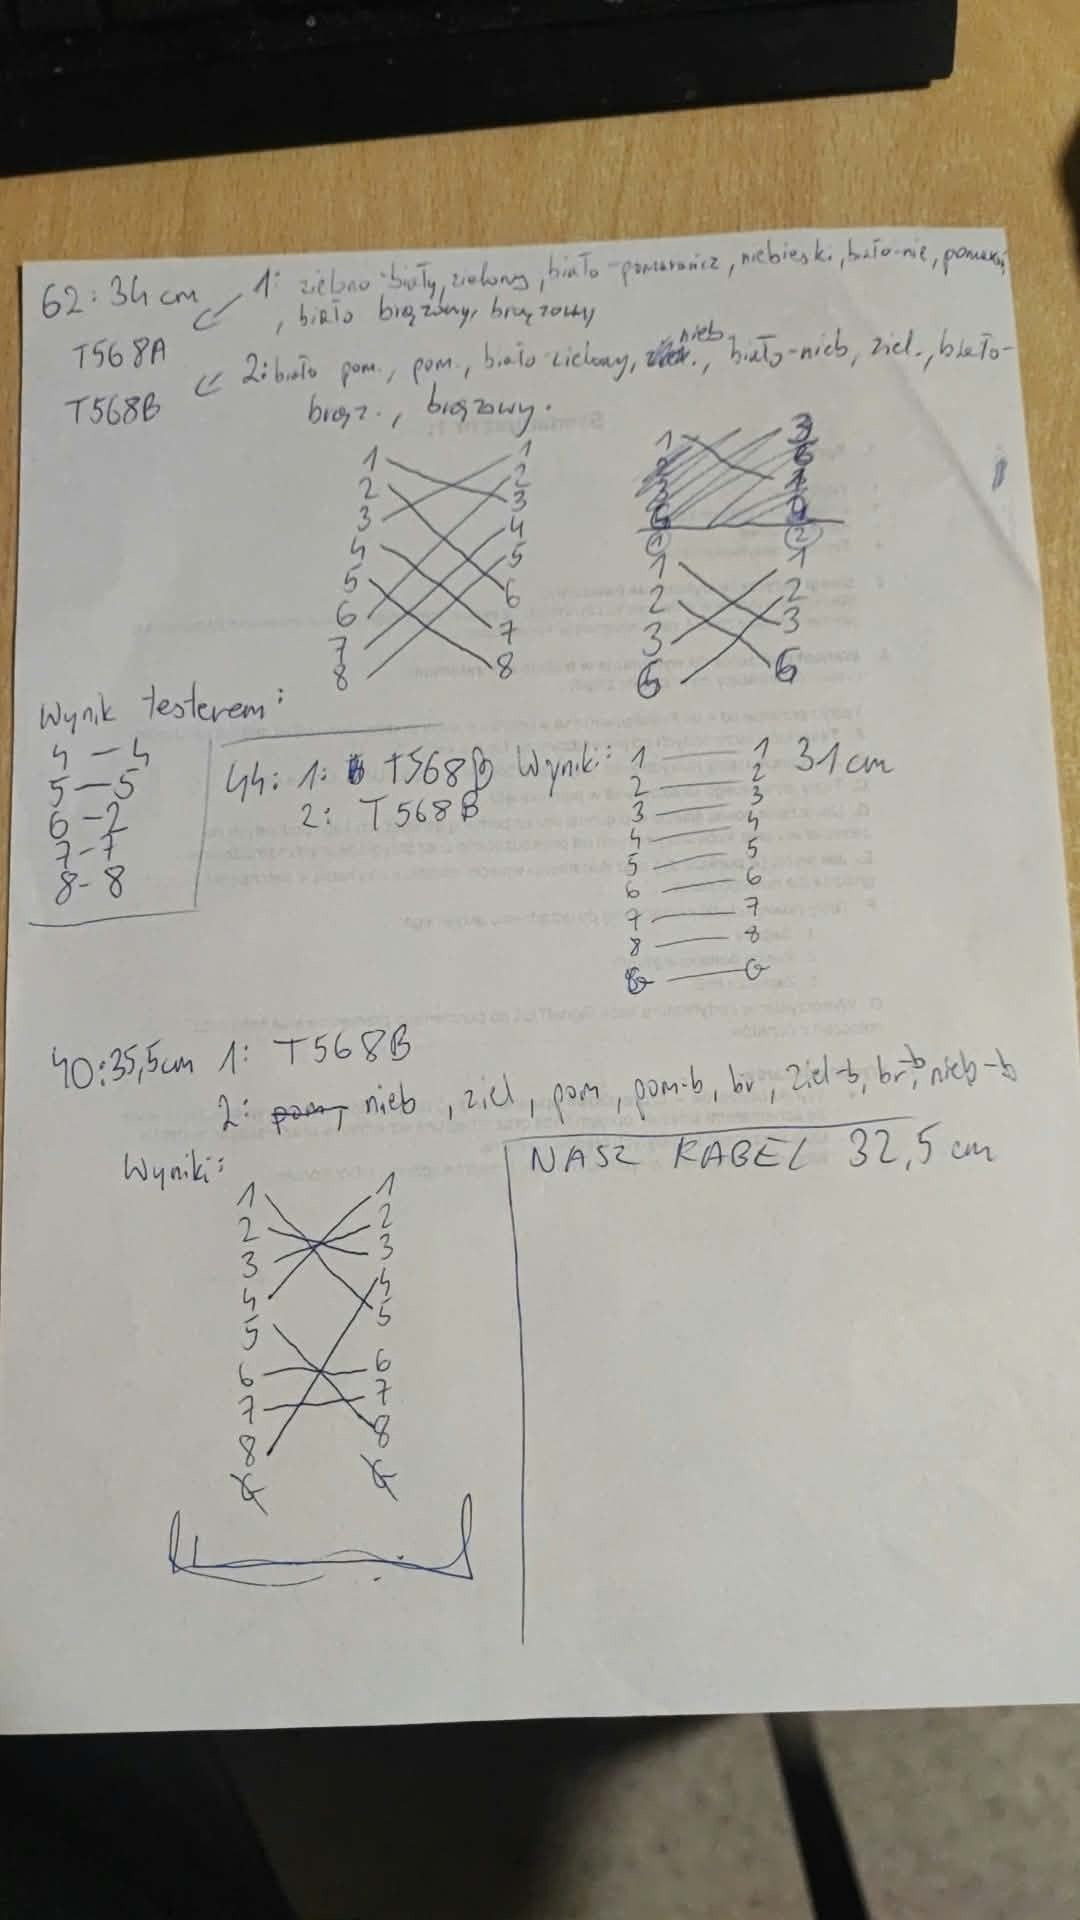
\includegraphics[width=0.72\textwidth]{notes_cables_62_40_60.jpg}
\caption{Ręczne schematy połączeń kabli nr 72, 60, 62, 44 i 40}
\end{figure}

\begin{figure}[H]
\centering
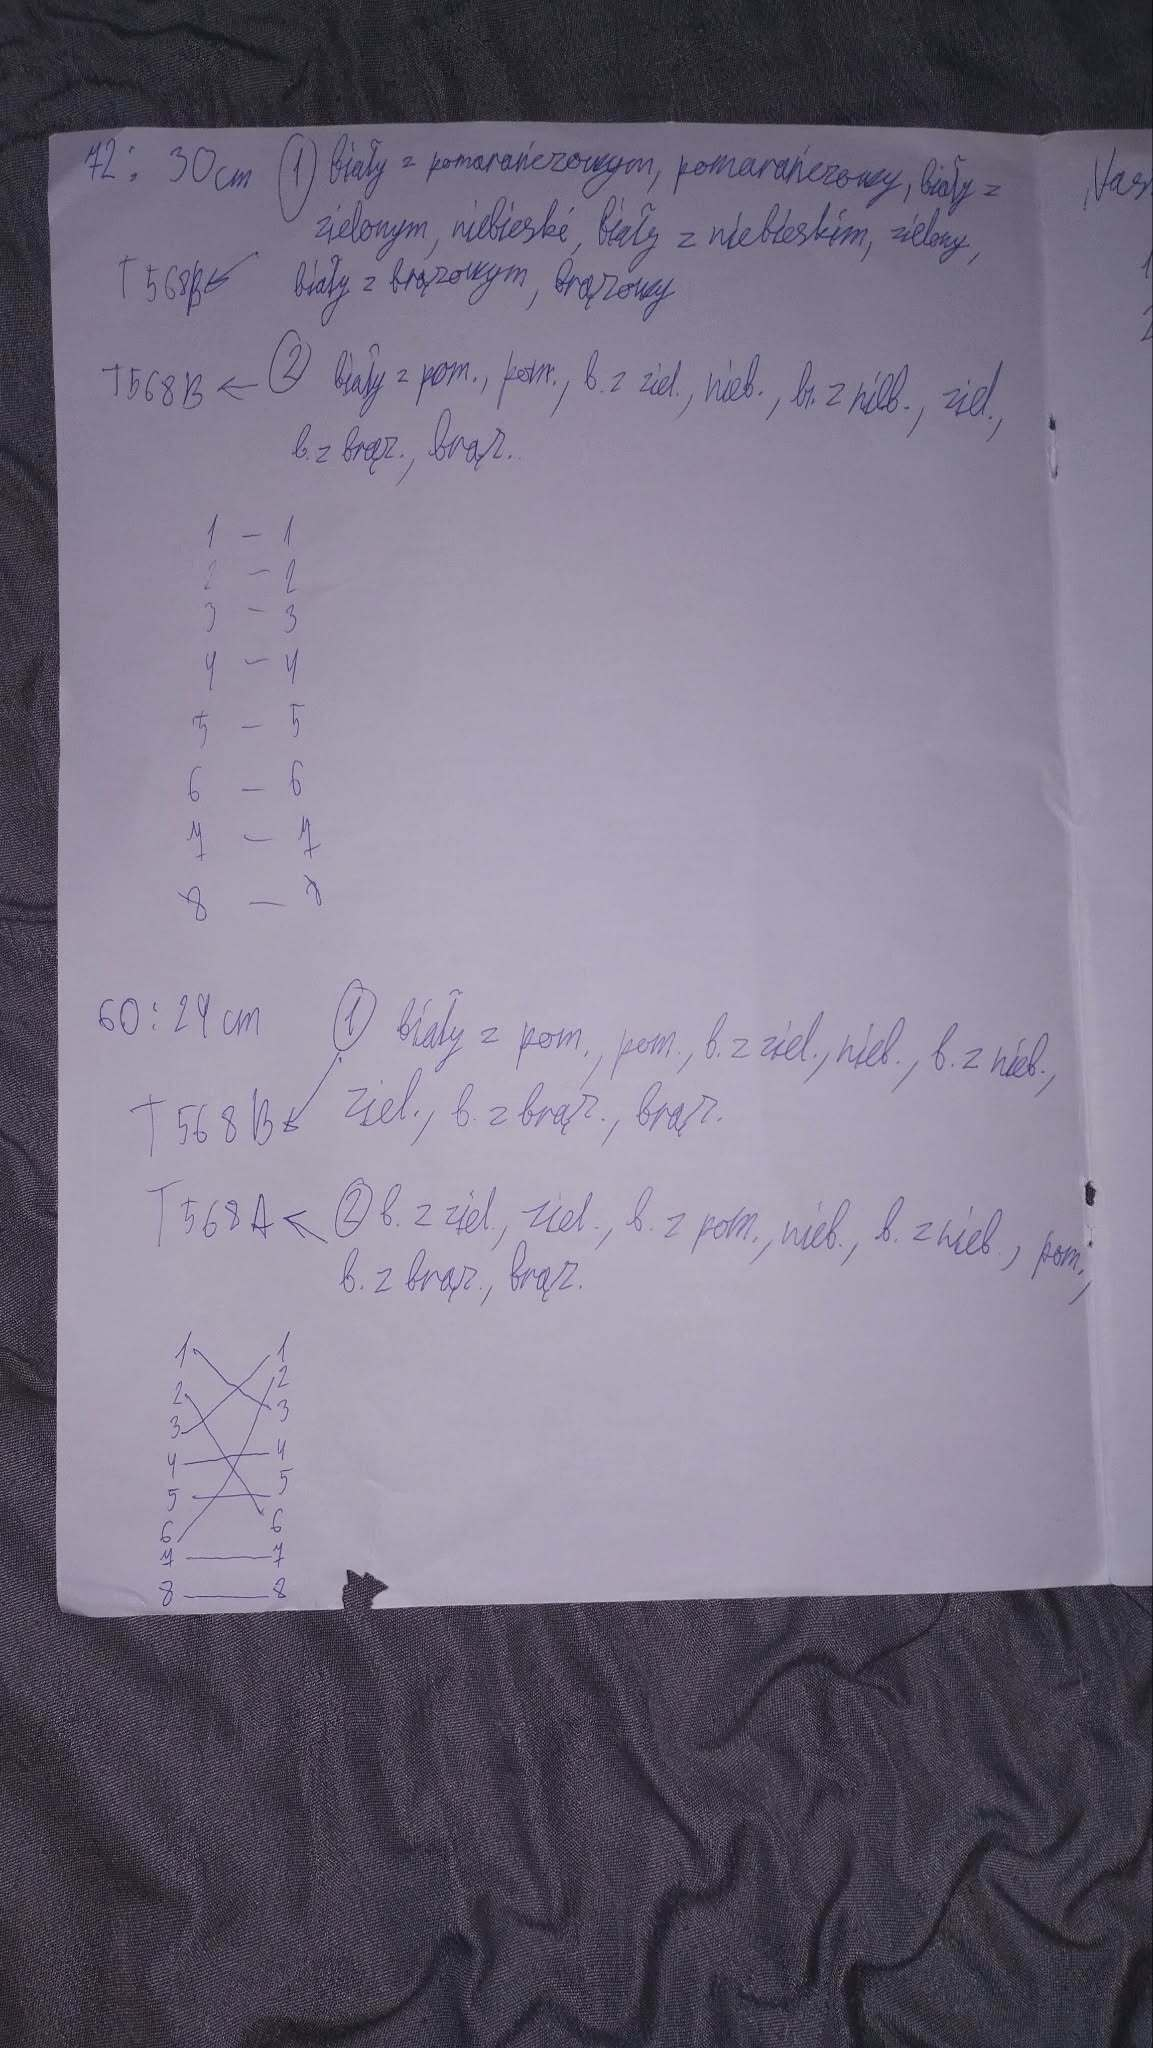
\includegraphics[width=0.72\textwidth]{notes_cable_numbers_lengths.jpg}
\caption{Ręczna notatka: numery kabli, długości oraz kolejność żył obu końcówek}
\end{figure}

\subsection{Zaciskanie i test nowych kabli}
Z każdego przygotowanego kabla ściągnęliśmy około 30 mm zewnętrznej izolacji. Następnie rozkręciliśmy żyły i uporządkowaliśmy je według standardu T568B:
\[
1=\text{biało-pomarańczowy},\quad
2=\text{pomarańczowy},\quad
3=\text{biało-zielony},\quad
4=\text{niebieski},
\]
\[
5=\text{biało-niebieski},\quad
6=\text{zielony},\quad
7=\text{biało-brązowy},\quad
8=\text{brązowy}.
\]
Żyły wyrównaliśmy i przycięliśmy do długości około 12--13 mm, a następnie wsunęliśmy je do wtyczki tak, aby miedziane końcówki dotarły do mechanizmu zaciśnięcia, a plastikowy zacisk znalazł się na zewnętrznej izolacji. Po zaciśnięciu drugiej końcówki przeprowadziliśmy test.

\begin{figure}[H]
\centering
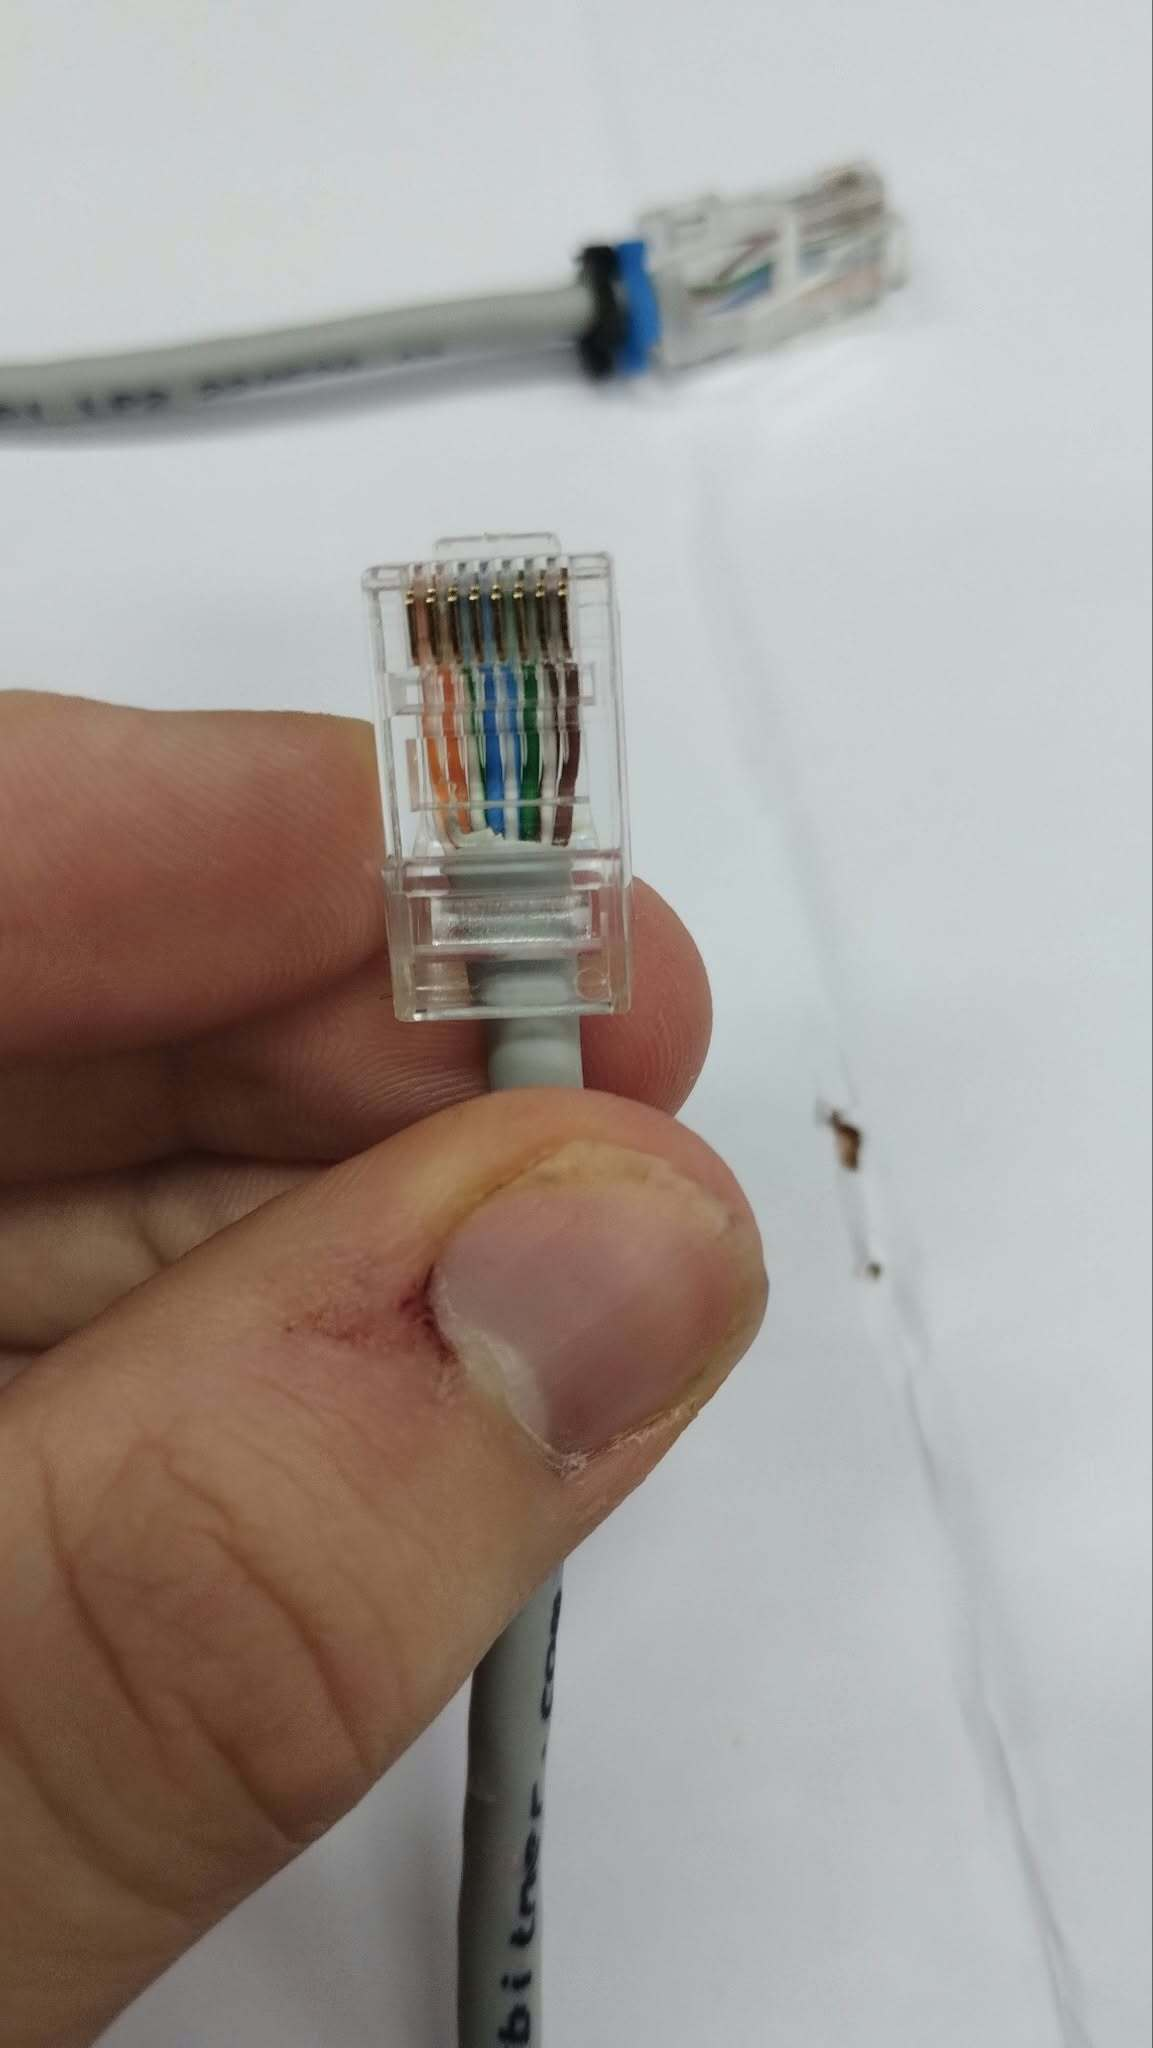
\includegraphics[width=0.55\textwidth]{rj45_prepared_connector.jpg}
\caption{Widok zaciśniętej wtyczki RJ45: osiem żył w kolejności widocznej od strony styków}
\end{figure}

\begin{figure}[H]
\centering
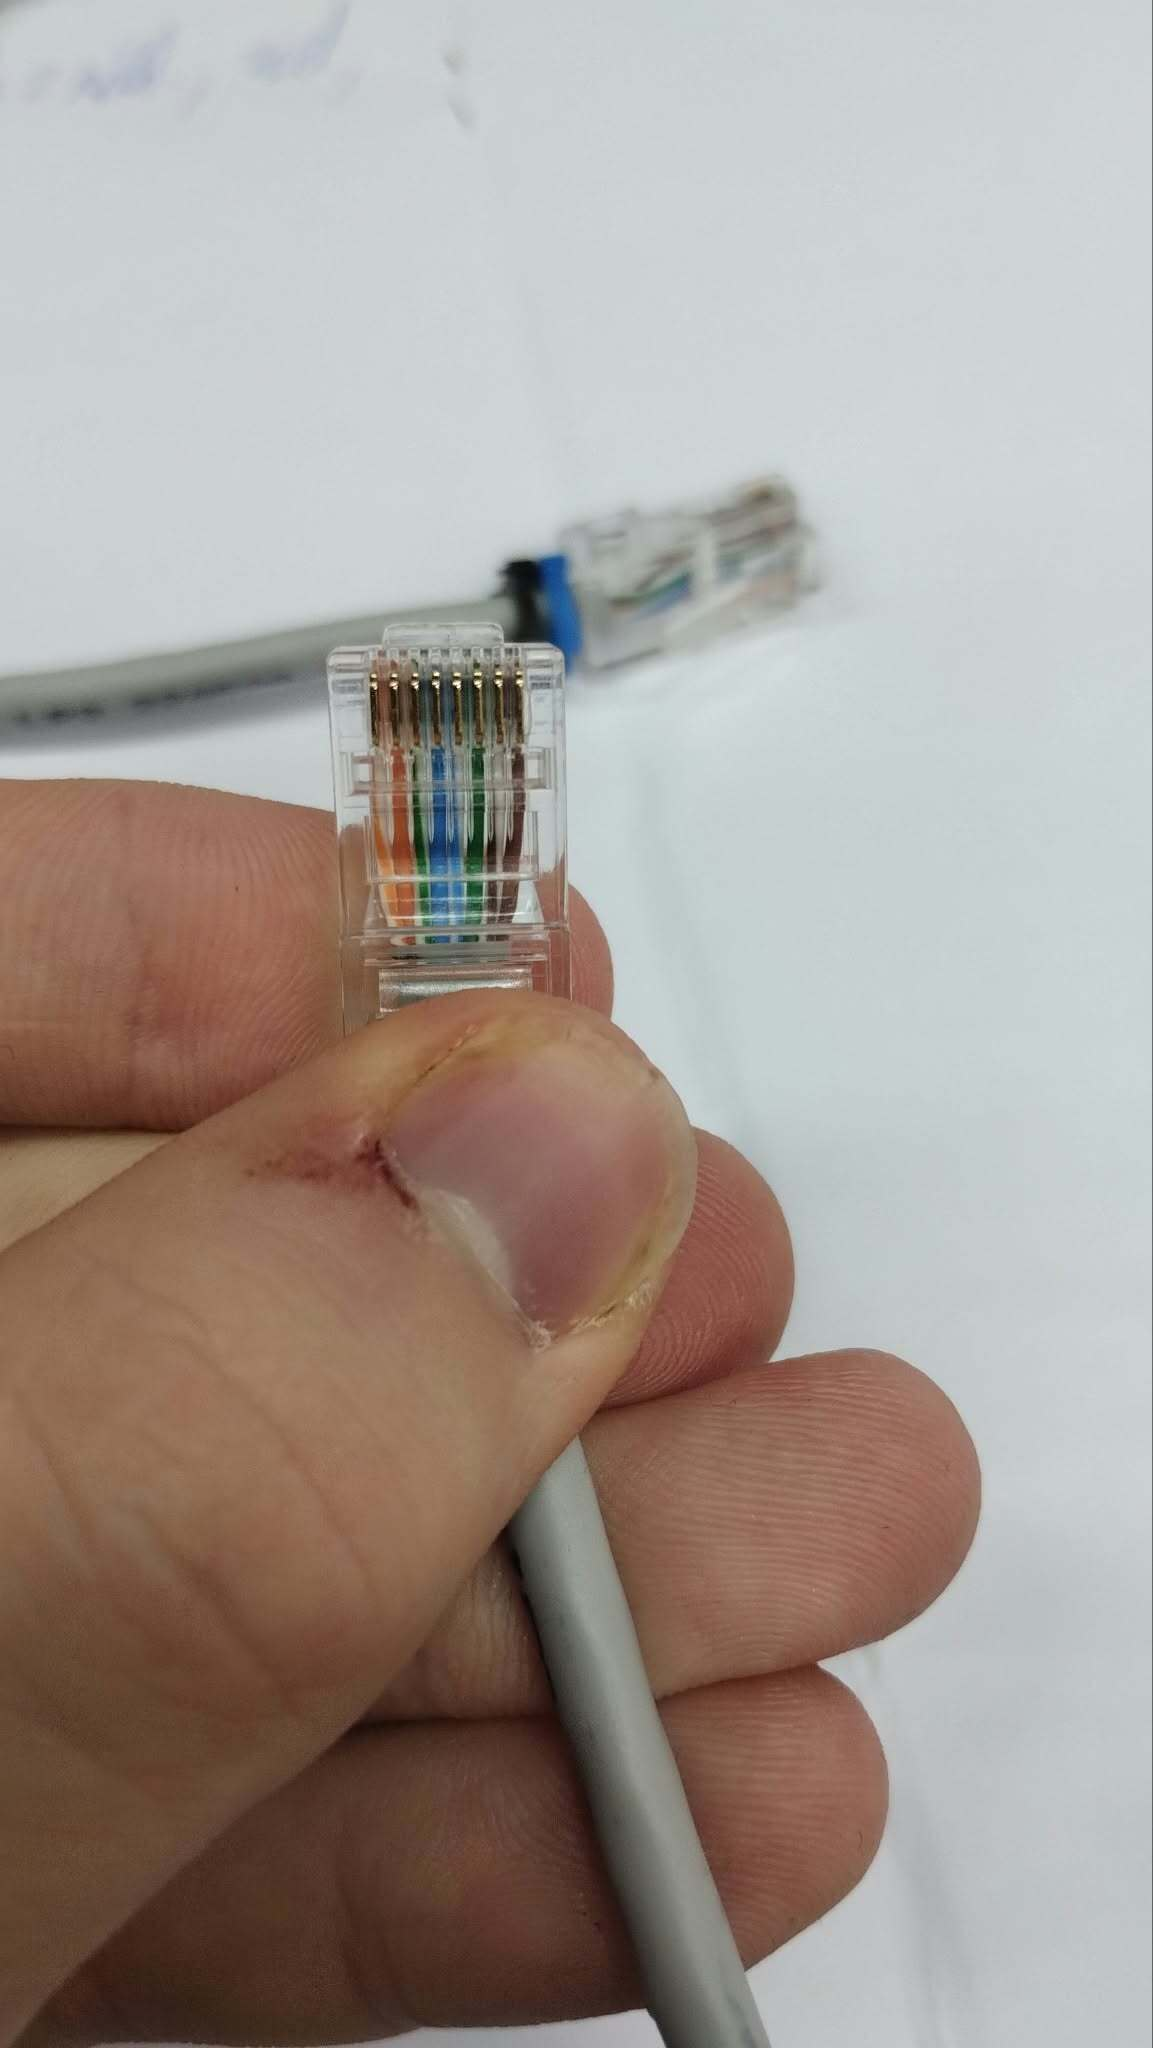
\includegraphics[width=0.55\textwidth]{rj45_connector_from_wire_side.jpg}
\caption{Szczegół zaciśniętej wtyczki RJ45 od strony przewodów}
\end{figure}

\begin{figure}[H]
\centering
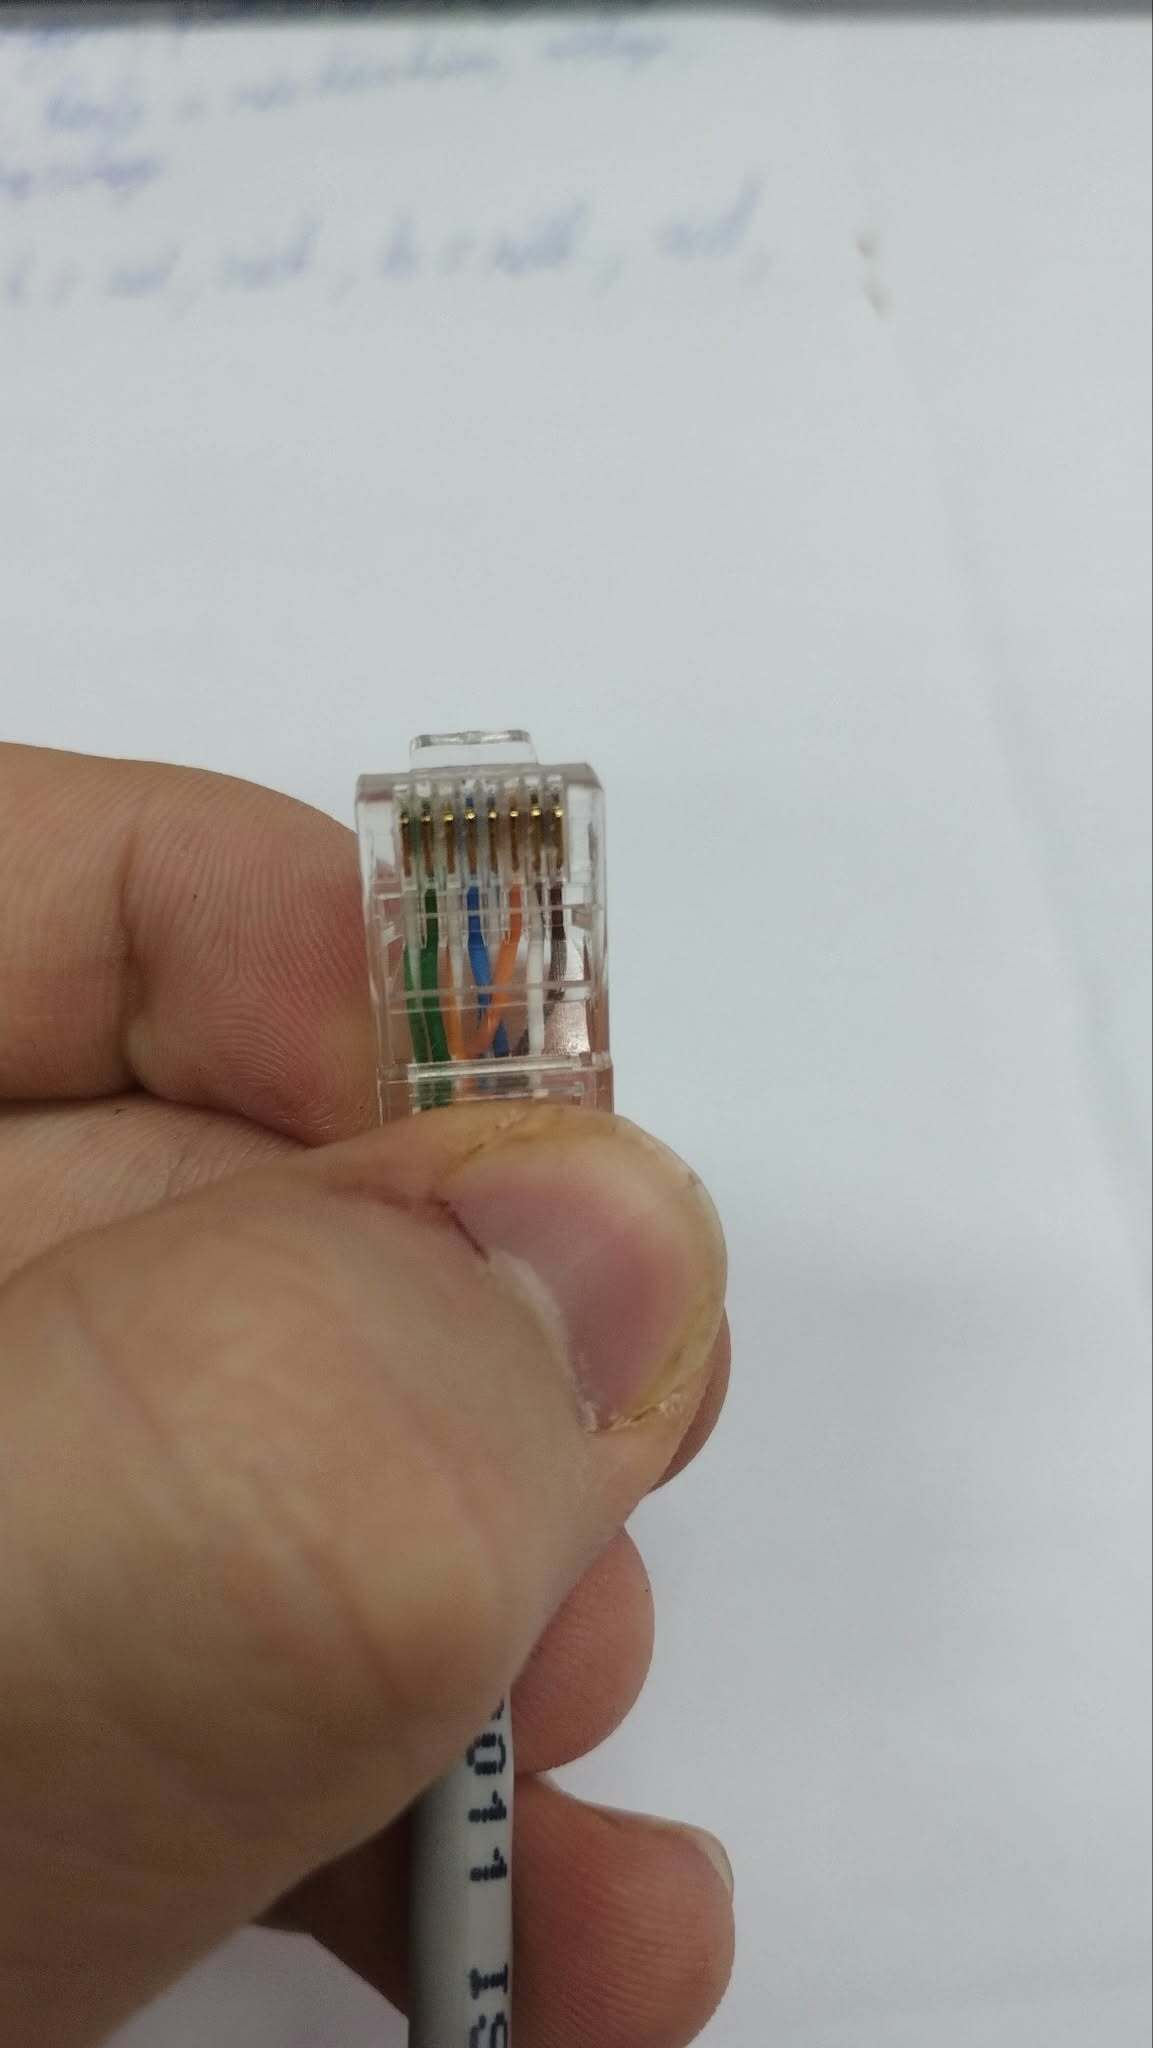
\includegraphics[width=0.55\textwidth]{patchcord_rj45_control.jpg}
\caption{Kontrola ustawienia przewodów w przeźroczystej wtyczce patchcorda}
\end{figure}

\subsection{Test istniejącego okablowania patchpanelu}
Do testów wykorzystaliśmy patchpanel i dobrej jakości patchcordy. W pierwszym pomiarze Fluke CableIQ wykrywał kabel i wyświetlał informacje o 1000BASE-T. Tester mierzył długość, mapę przewodów i oceniał pary.

\begin{figure}[H]
\centering
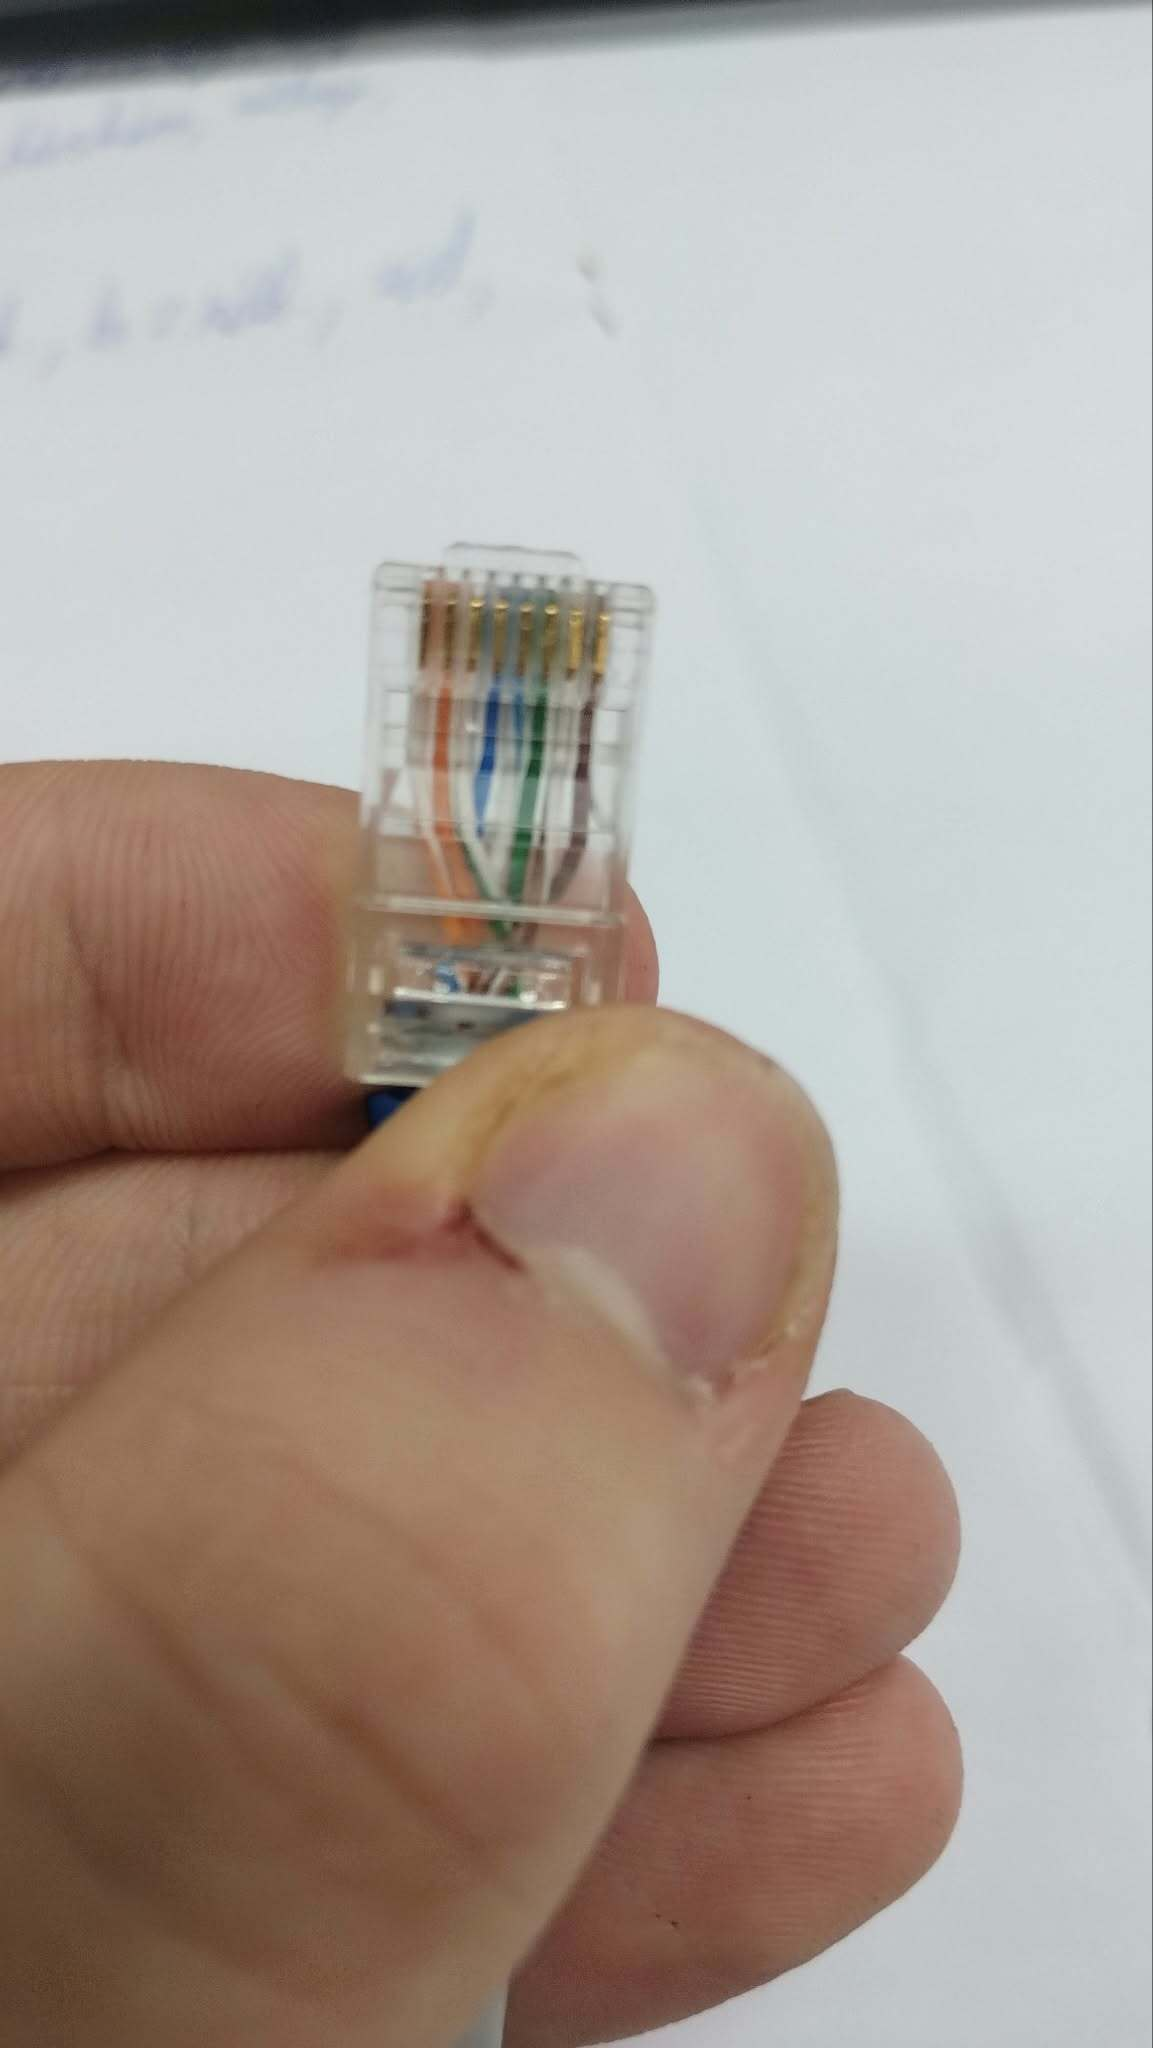
\includegraphics[width=0.55\textwidth]{patchcord_finished_connector.jpg}
\caption{Kontrola wykonanej końcówki RJ45 i ustawienia żył przed testem}
\end{figure}

\begin{figure}[H]
\centering
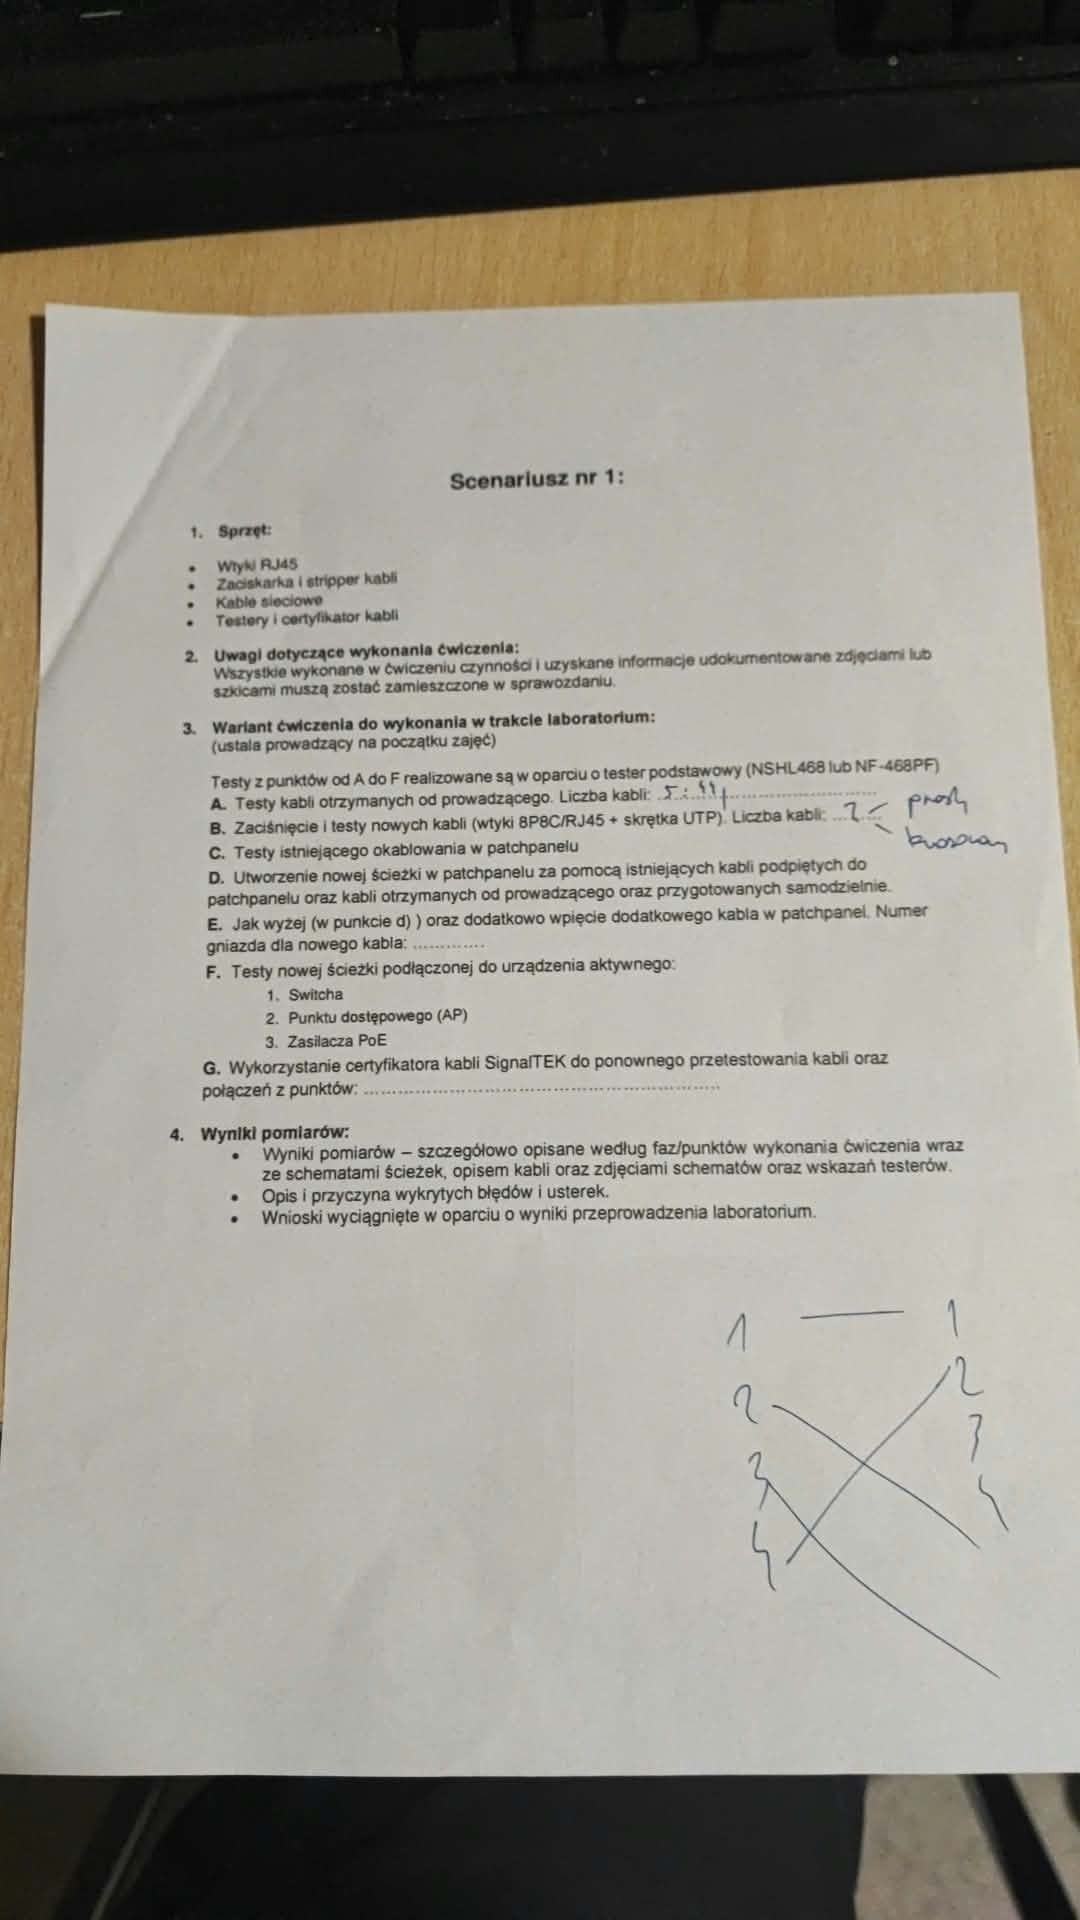
\includegraphics[width=0.72\textwidth]{lab_scenario_and_connection_drawing.jpg}
\caption{Ręczny schemat scenariusza nr 1 oraz propozycja konfiguracji ścieżki}
\end{figure}

\subsection{Budowa nowej ścieżki}
Na podstawie istniejącego okablowania i przygotowanych przez nas patchcordów złożyliśmy nową ścieżkę między gniazdami patchpanelu. Każdy etap kończyliśmy testem przed wprowadzeniem kolejnego elementu, co pozwoliło nam odróżnić błąd patchcorda od błędu patchpanelu lub nowego kabla.

\subsection{Wpięcie kabla do tylnej części patchpanelu}
Jeżeli kabel nie był zakończony wtyczką, zaciśnęliśmy wtyczkę według T568B. Przy wpinaniu do tylnej części patchpanelu porównaliśmy standard wtyczki z numeracją pinów i dopasowaliśmy pary do właściwego gniazda. Na zdjęciach zachowaliśmy zgodność między paramami 1--2, 3--6, 4--5 i 7--8.

\subsection{Test ścieżki z urządzeniem aktywnym}
W punkcie F ścieżkę zakończono urządzeniem aktywnym. Zdjęcia obejmują przełącznik/obudowę po stronie aktywnej oraz kabel połączony z modulem terminatora. Taki układ pozwala sprawdzić połączenia miedziane i wykonać transmisję diagnostyczną.

\section{Wyniki pomiarów}
\subsection{Wyniki testera CableIQ -- kabel prosty}
Na zdjęciu \texttt{IMG\_20261110\_123759.jpg} widoczny jest ekran testu z trzema pozycjami:
\begin{itemize}
  \item 1000BASE-T -- potwierdzony,
  \item 100BASE-TX -- potwierdzony,
  \item 10BASE-T -- potwierdzony.
\end{itemize}

Zdjęcie \texttt{fluke\_signal\_length\_0\_2m.jpg} przedstawia pomiar parametrów sygnału i długości. Na ekranie widoczny jest wynik \textbf{0,2 m} dla krótkiego patchcorda. Kolejne zdjęcie potwierdziło kwalifikację \textbf{1000BASE-T} jako \textit{Qualified for 1000BASE-T}.

\begin{figure}[H]
\centering
\begin{minipage}{0.48\textwidth}
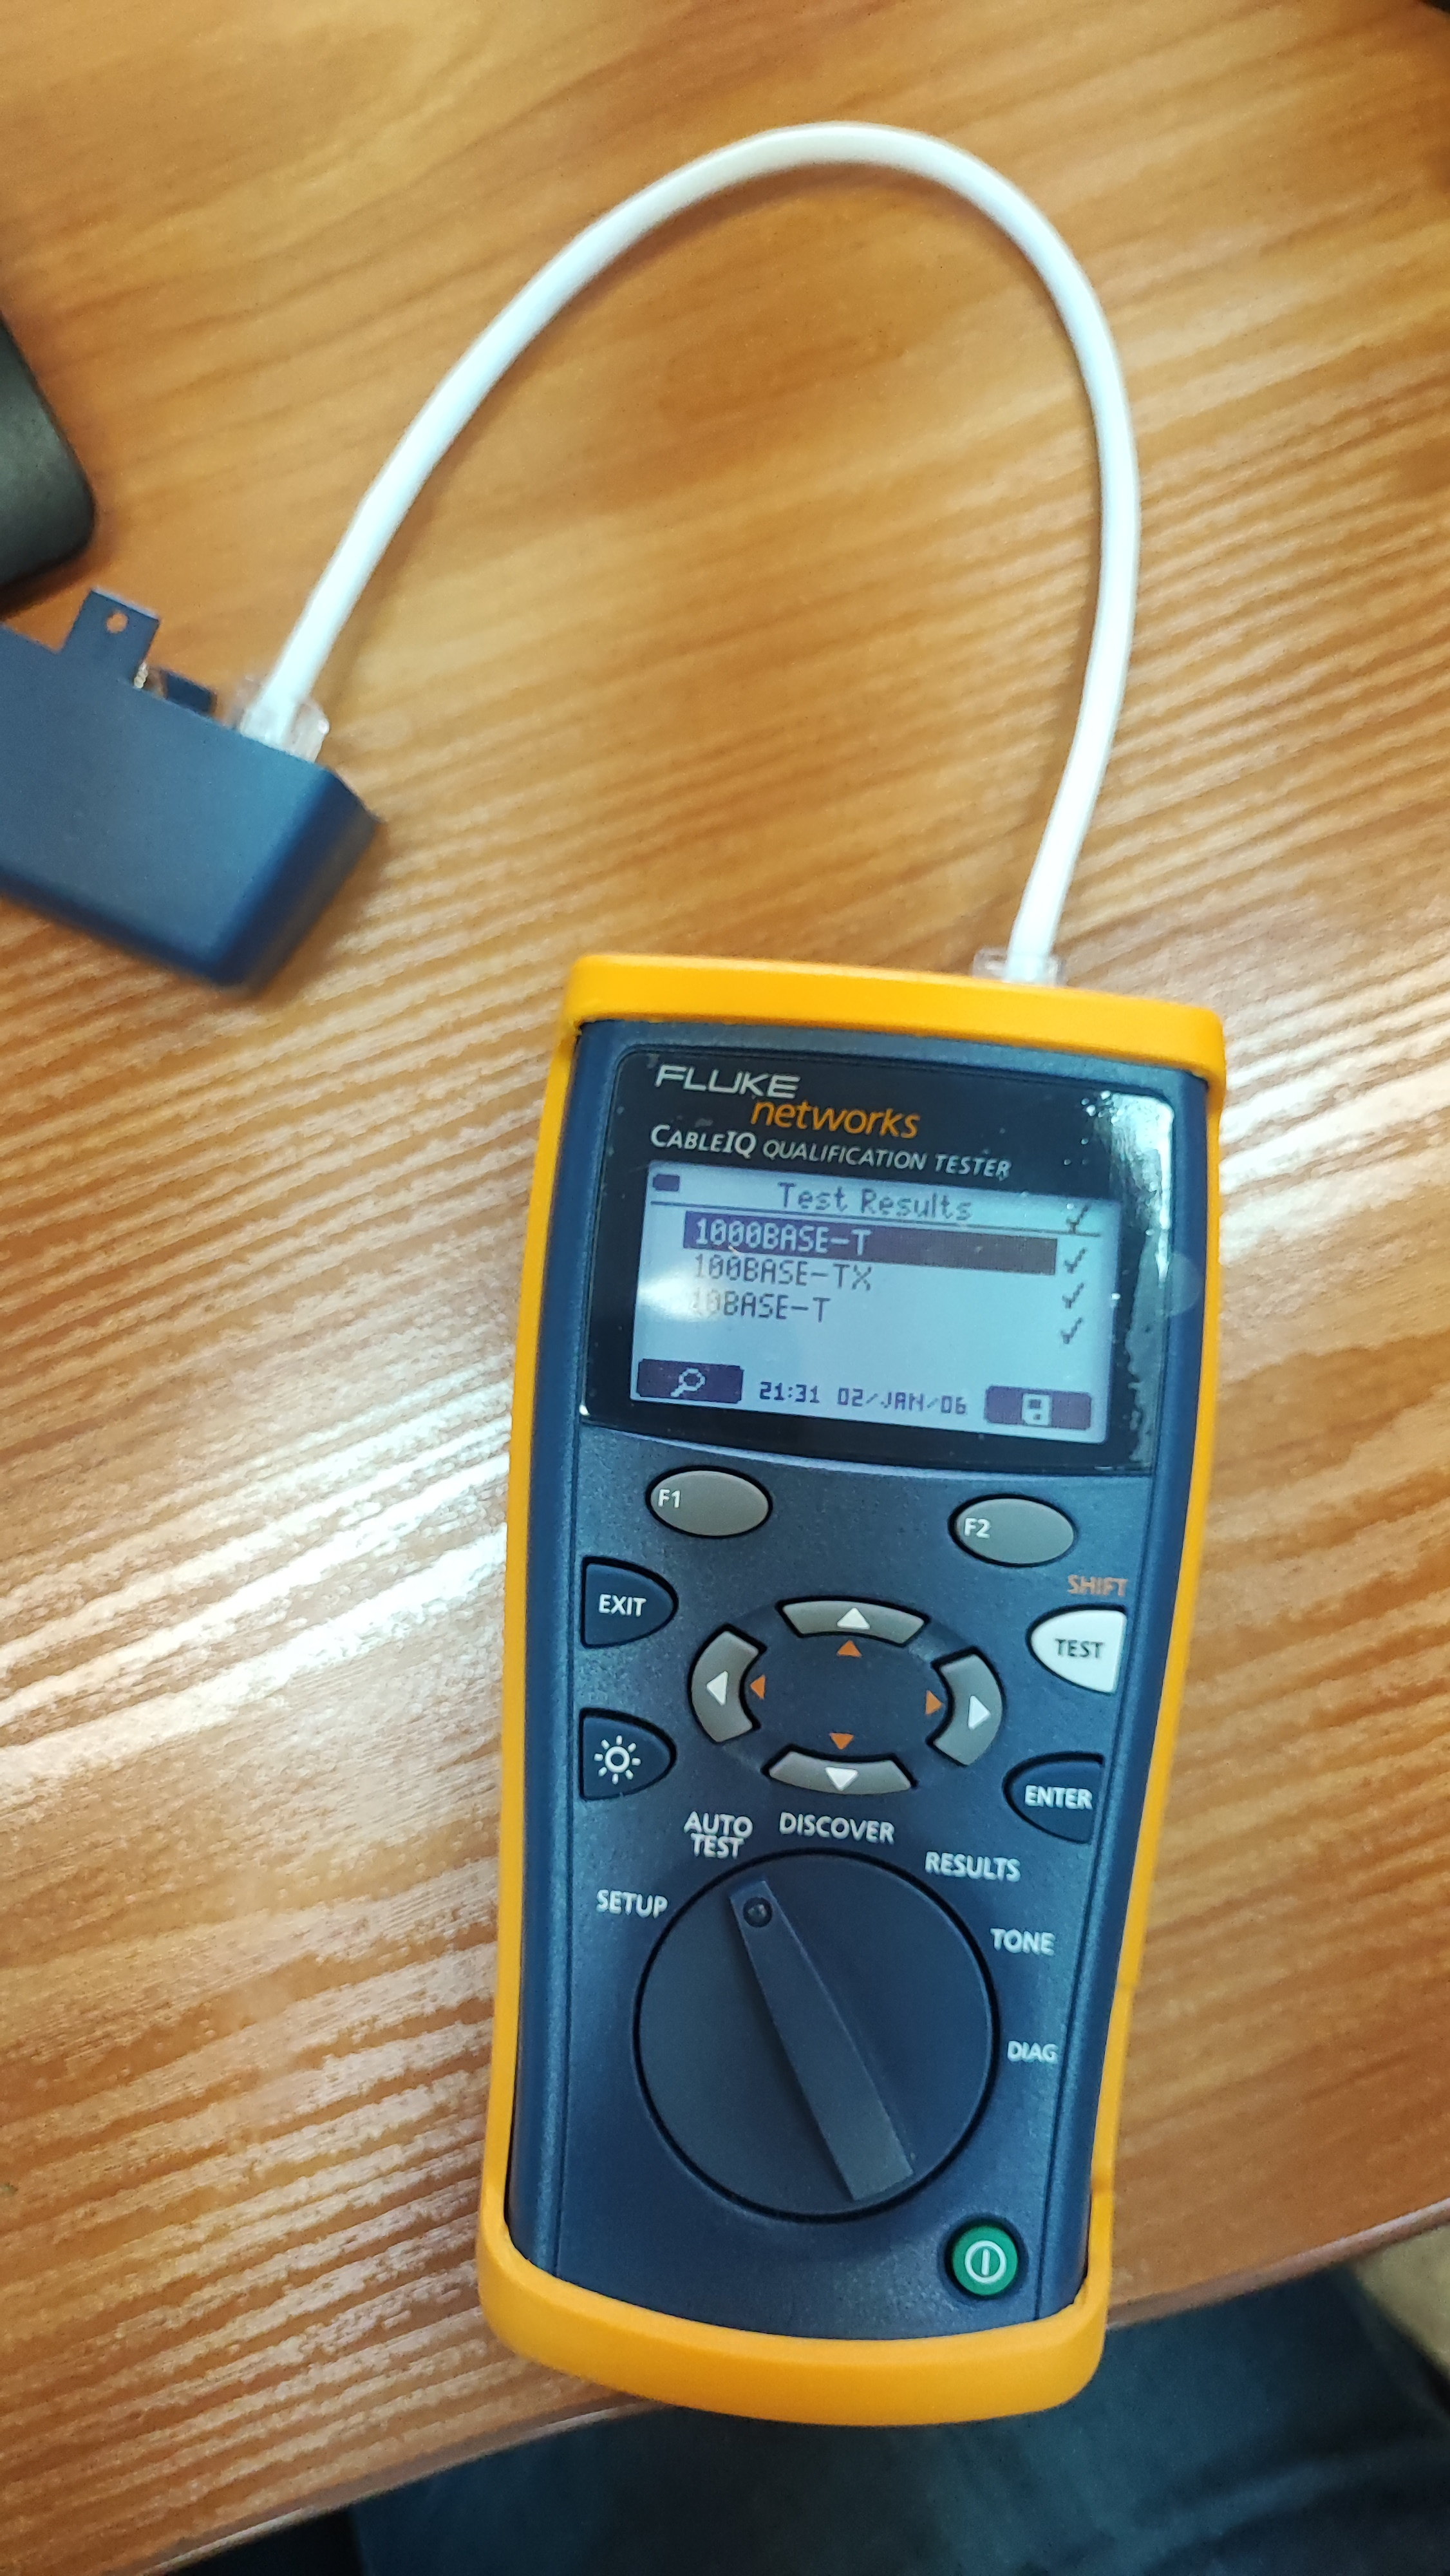
\includegraphics[width=\textwidth]{fluke_test_menu_1000_100_10.jpg}
\caption{Seria zdjęć: rozpoznanie standardów Ethernet przez CableIQ}
\end{minipage}\hfill
\begin{minipage}{0.48\textwidth}
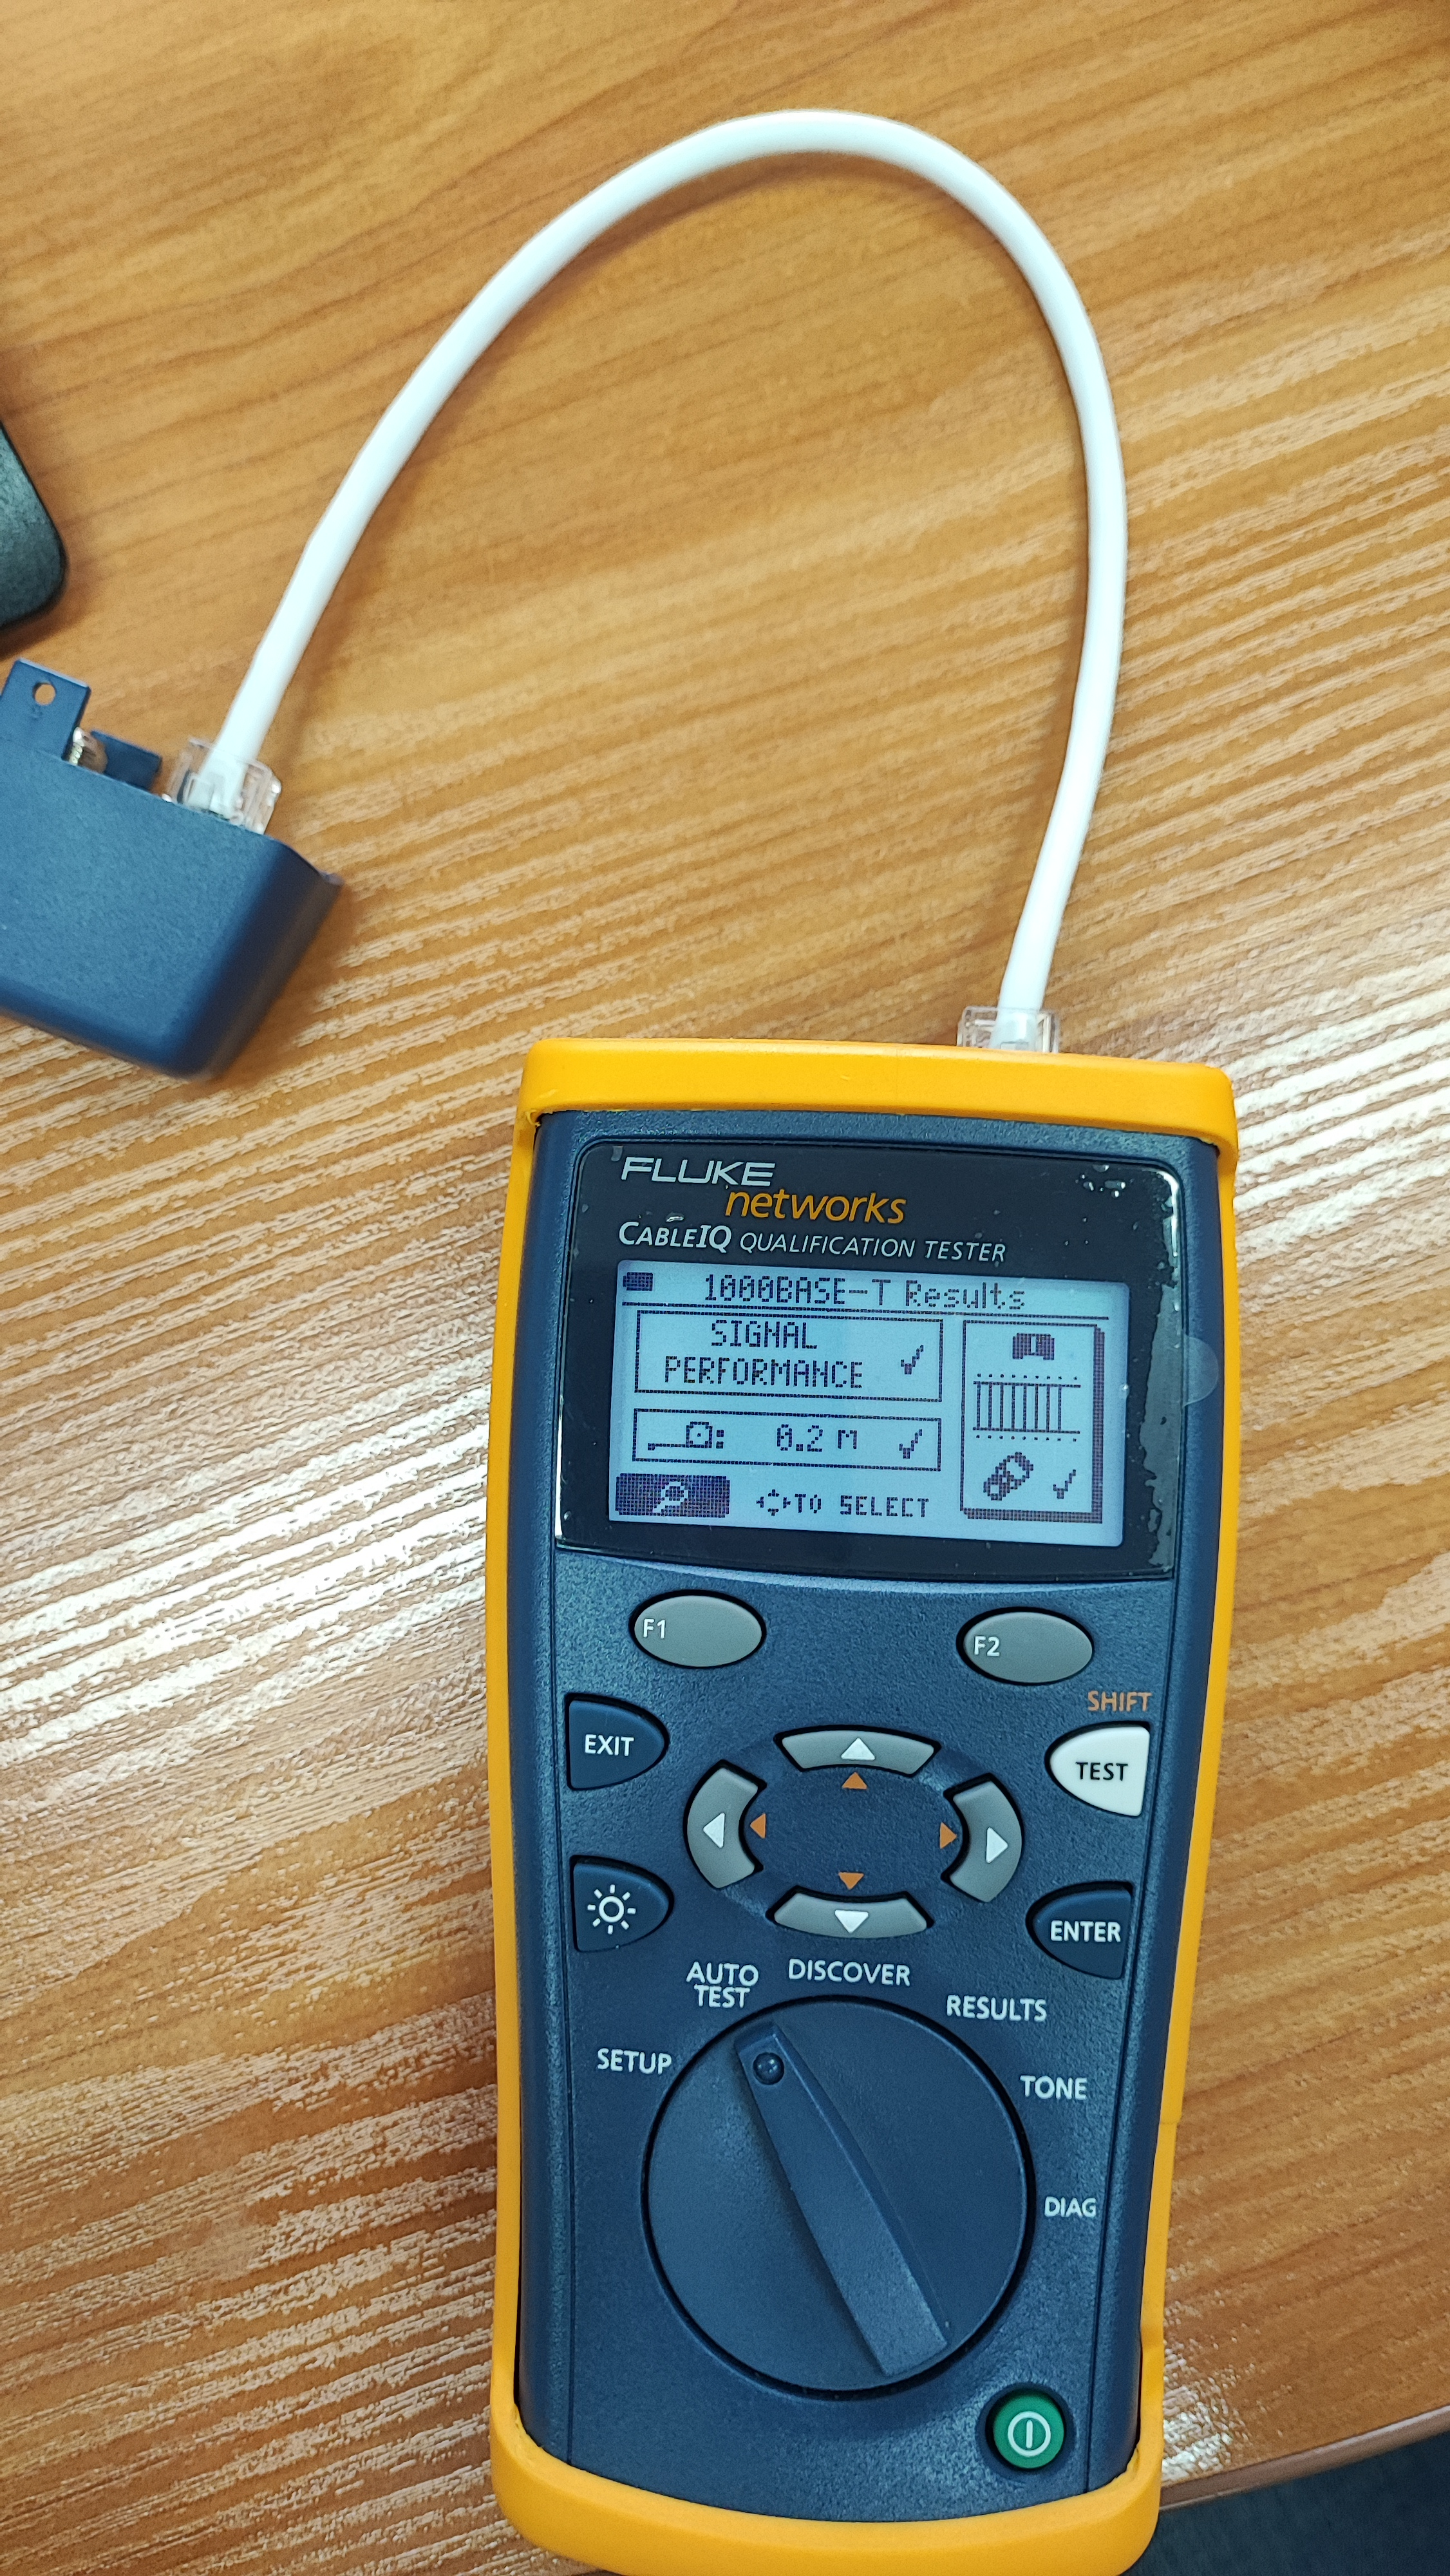
\includegraphics[width=\textwidth]{fluke_signal_length_0_2m.jpg}
\caption{Seria zdjęć: pomiar parametrów i długości patchcorda}
\end{minipage}
\end{figure}

\begin{figure}[H]
\centering
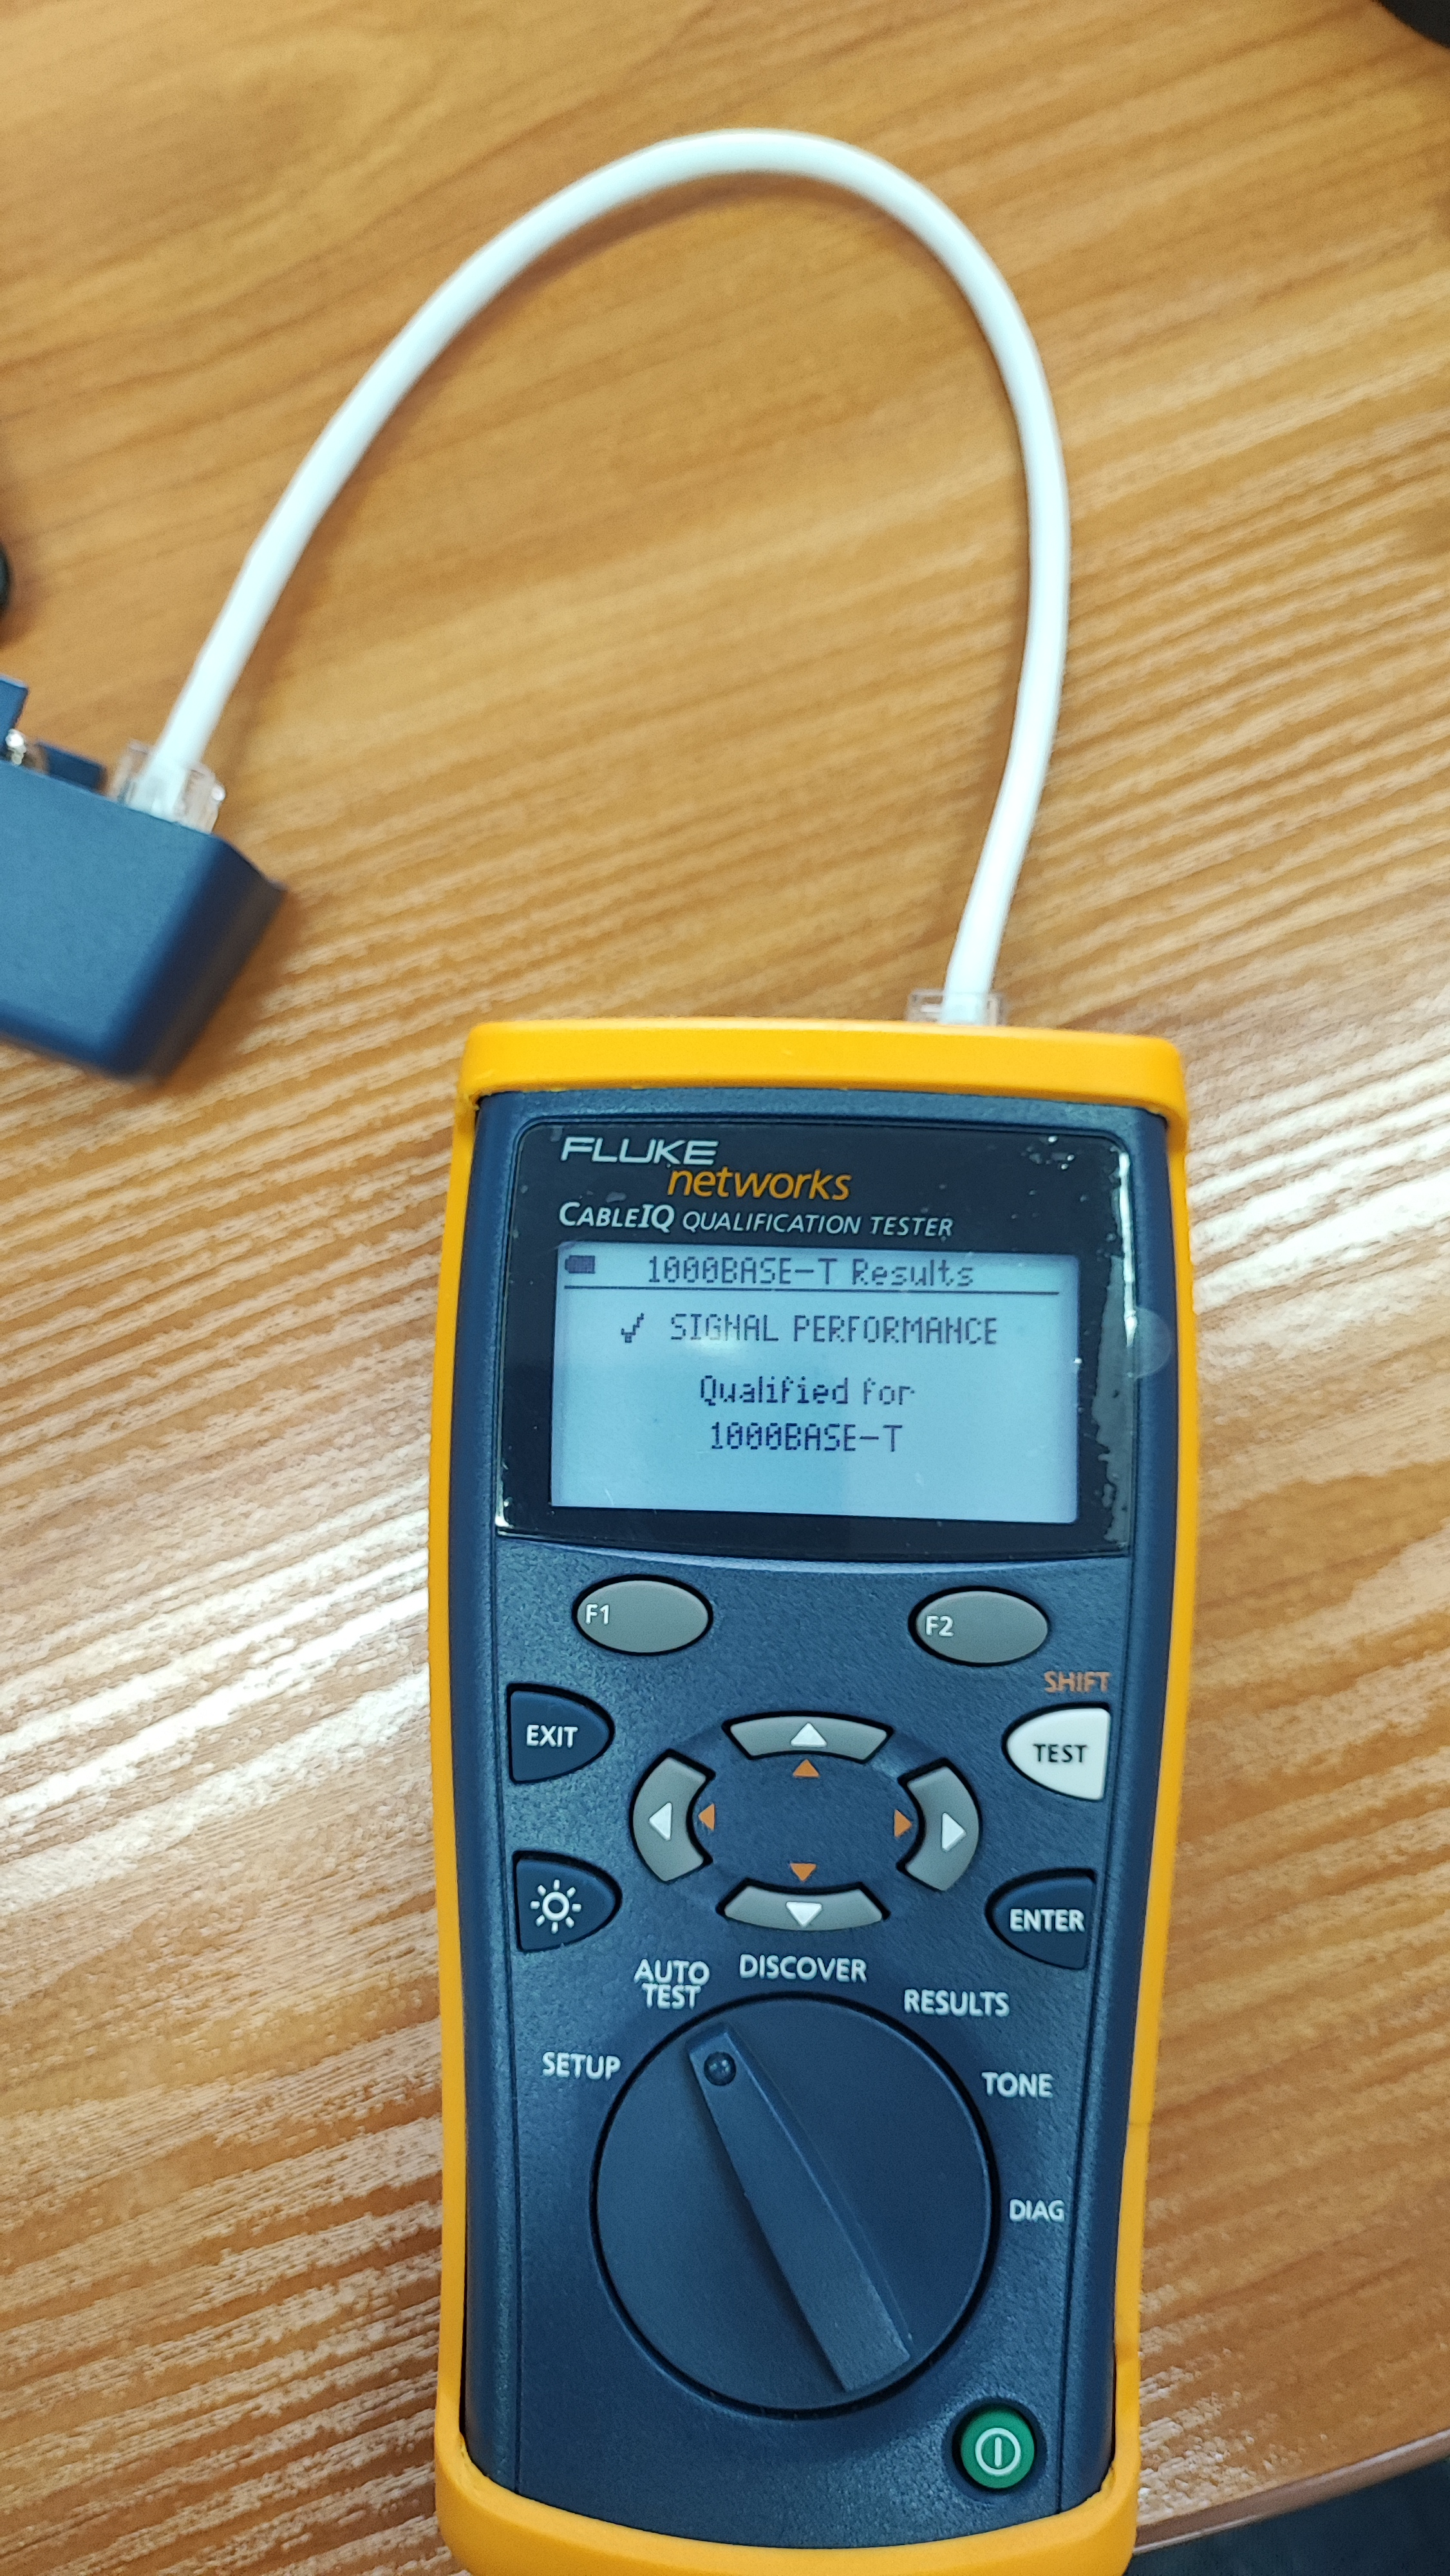
\includegraphics[width=0.58\textwidth]{fluke_qualified_1000base-t.jpg}
\caption{Seria zdjęć: wynik pozytywnej kwalifikacji kabla}
\end{figure}

\subsection{Mapa przewodów i długości par}
Zdjęcie \texttt{IMG\_20261110\_123831.jpg} pokazuje poprawną mapę przewodów: wszystkie osiem przewodów połączonych z pinami 1--8, bez przerwania ani skrzyżowania. Na \texttt{IMG\_20261110\_123842.jpg} podano długości par:
\[
1--2:\ 0,2\ \text{m},\qquad
3--6:\ 0,2\ \text{m},\qquad
4--5:\ 0,2\ \text{m},\qquad
7--8:\ 0,2\ \text{m}.
\]
Na podstawie widocznych pomiarów był to bardzo krótki patchcord. Nie przypisywaliśmy mu innych długości, których nie potwierdzają zdjęcia.

\begin{figure}[H]
\centering
\begin{minipage}{0.48\textwidth}
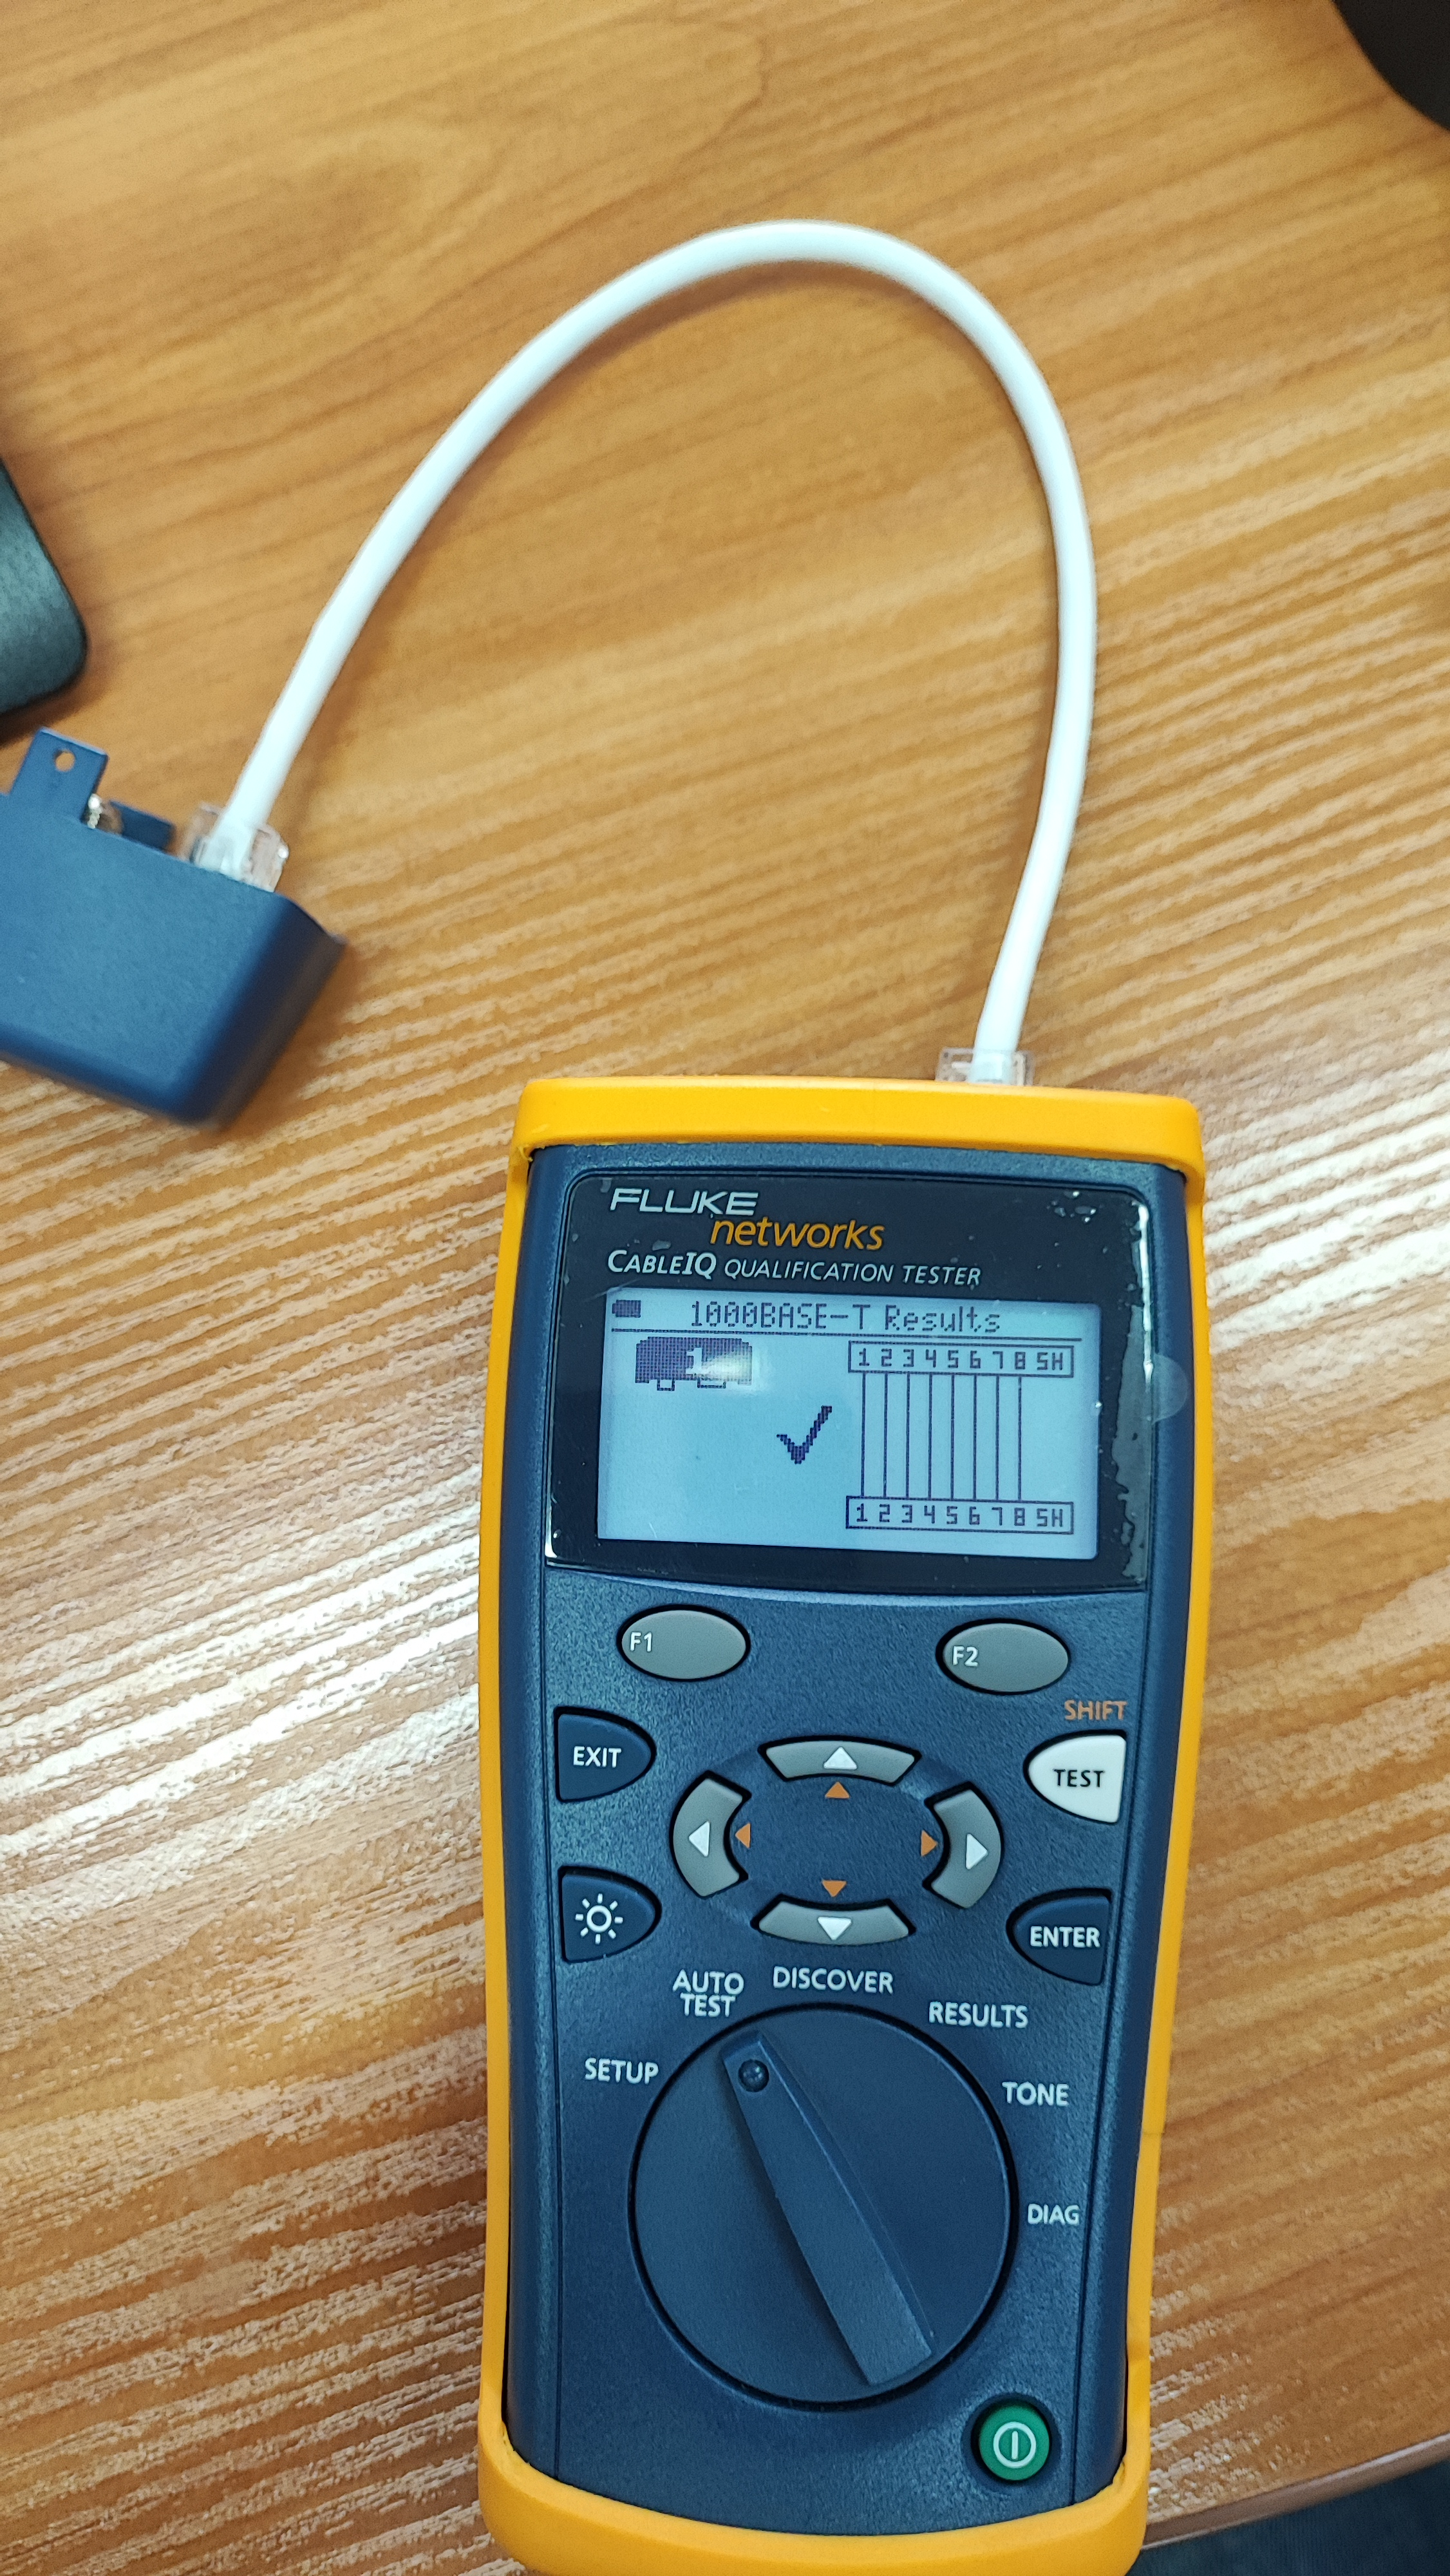
\includegraphics[width=\textwidth]{fluke_wiremap_correct.jpg}
\caption{Seria zdjęć: poprawna mapa przewodów}
\end{minipage}\hfill
\begin{minipage}{0.48\textwidth}
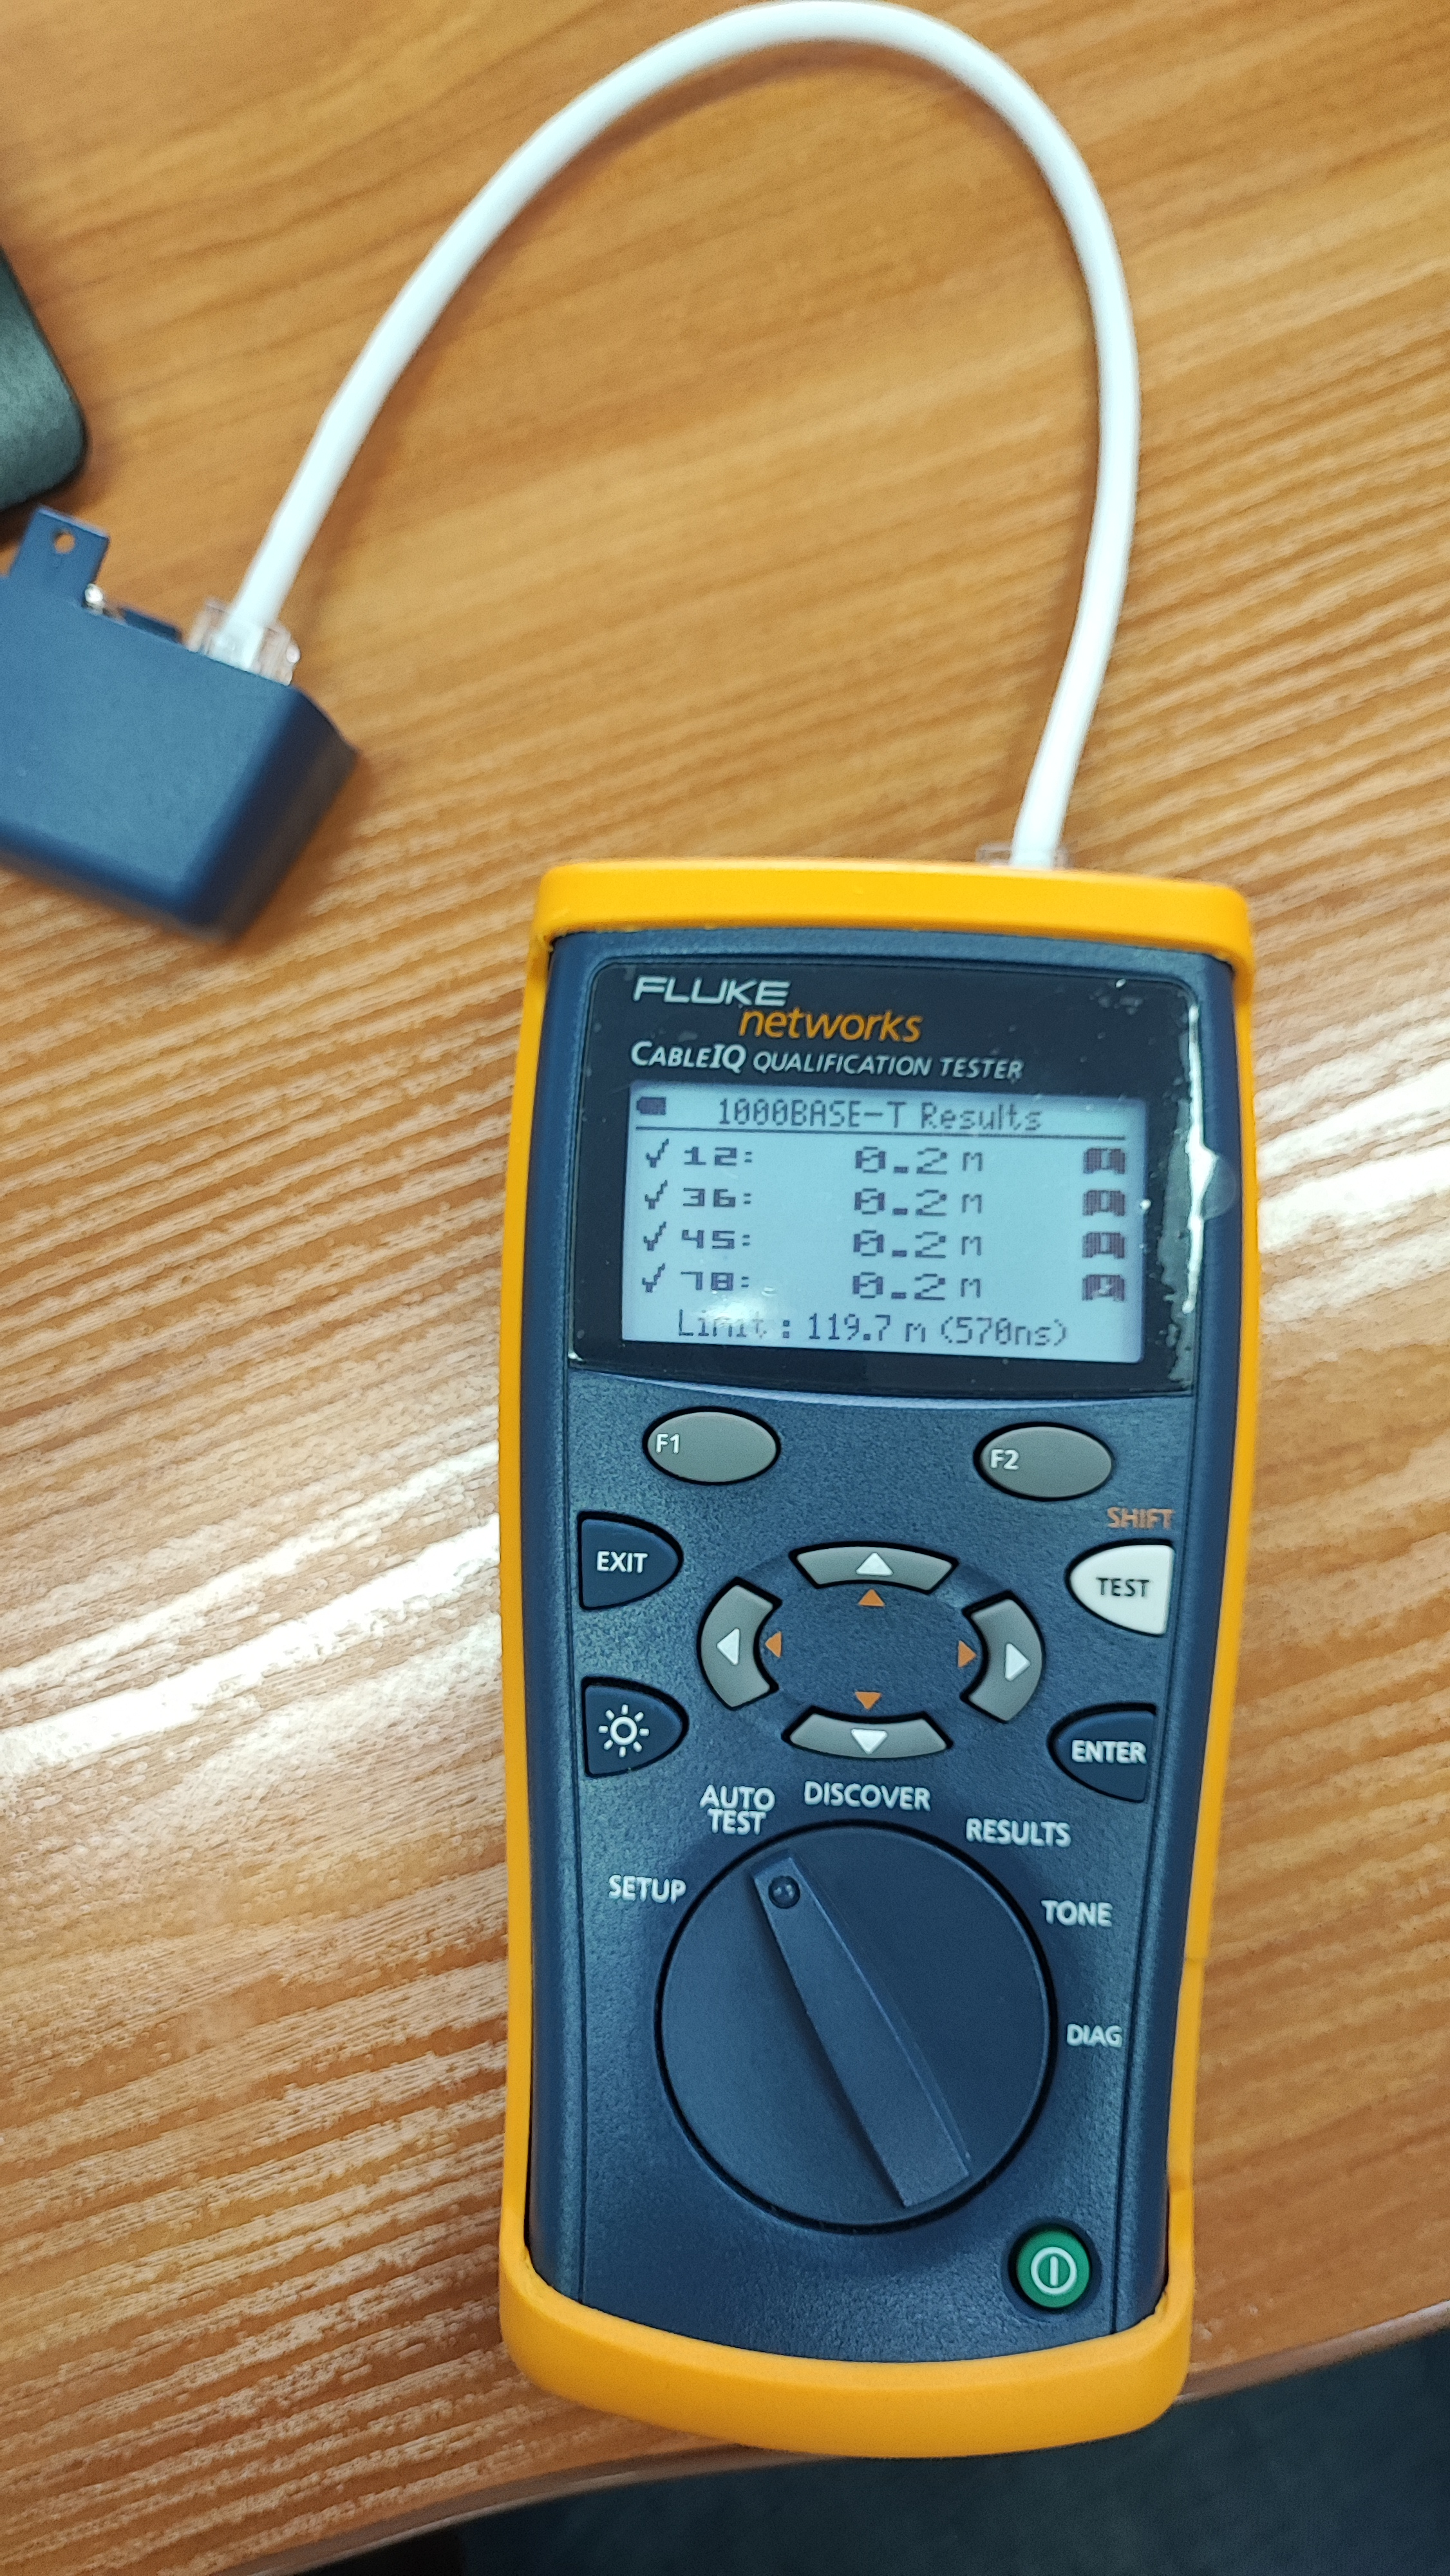
\includegraphics[width=\textwidth]{fluke_pairs_lengths_0_2m.jpg}
\caption{Seria zdjęć: długości par badanego próbnego kabla}
\end{minipage}
\end{figure}

\subsection{Dalsze testy patchcordów i ścieżek}
Zdjęcia od \texttt{124127.jpg} do \texttt{124538.jpg} dokumentują kolejne pozycje pomiarowe. Ich wspólna interpretacja przedstawia się następująco:
\begin{itemize}
  \item \texttt{124127}: mapa par 1--2, 3--6, 4--5 i 7--8 została zachowana; długości wynosiły około 0,1 m.
  \item \texttt{124242}: pomiar kolejnych par; wartości 0,1--0,2 m mieszczą się w klasie krótkiego patchcorda.
  \item \texttt{124400--124421}: kolejne pomiary długości i wyników standardów 100BASE-T/1000BASE-T.
  \item \texttt{124458--124538}: pojawiły się stany \textit{Wiring fault} i \textit{Hot tested}, co oznaczało błąd wykonania połączenia lub test kabla do momentu stabilizacji sygnału.
\end{itemize}

Testy \texttt{124458} i \texttt{124530} wskazują, że nie wszystkie badane ścieżki były poprawne. Dodatkowo \texttt{124538} przedstawia graficzną mapę błędu, w której linie par krzyżują się i nie tworzą jednej prawidłowej topologii.

\begin{table}[H]
\centering
\small
\begin{tabularx}{\textwidth}{>{\centering\arraybackslash}p{0.15\textwidth}|>{\centering\arraybackslash}p{0.15\textwidth}|>{\centering\arraybackslash}p{0.17\textwidth}|X}
\toprule
\textbf{Nr próbnego kabla} & \textbf{Długość} & \textbf{Status} & \textbf{Interpretacja} \\
\midrule
Kabel nr 72 & 30 cm & Wiremap & Poprawna mapa przewodów i połączenie prosty. \\
Kabel nr 60 & 29 cm & Wiremap / crossover & Kabel krosowany; wynik porównano z końcówkami T568B i T568A. \\
Kabel nr 62 & 34 cm & Kwalifikacja i standardy & Rozpoznano 10BASE-T, 100BASE-TX i 1000BASE-T. \\
Kabel nr 44 & 31 cm & Qualified / masa G & Kabel prosty, spełnienie 1000BASE-T potwierdzono. \\
Kabel nr 40 & 35,5 cm & Wiremap / masa G & Połączenie przeplatane, wymagające korekty kolejności żył. \\
Ścieżka z usterką & -- & Wiring fault & Nieprawidłowa realizacja połączenia. \\
Ścieżka z usterką & -- & Wiring fault & Należy sprawdzić końcówki i kolejność żył. \\
\bottomrule
\end{tabularx}
\caption{Zestawienie wyników pomiarów Fluke CableIQ}
\end{table}

\begin{figure}[H]
\centering
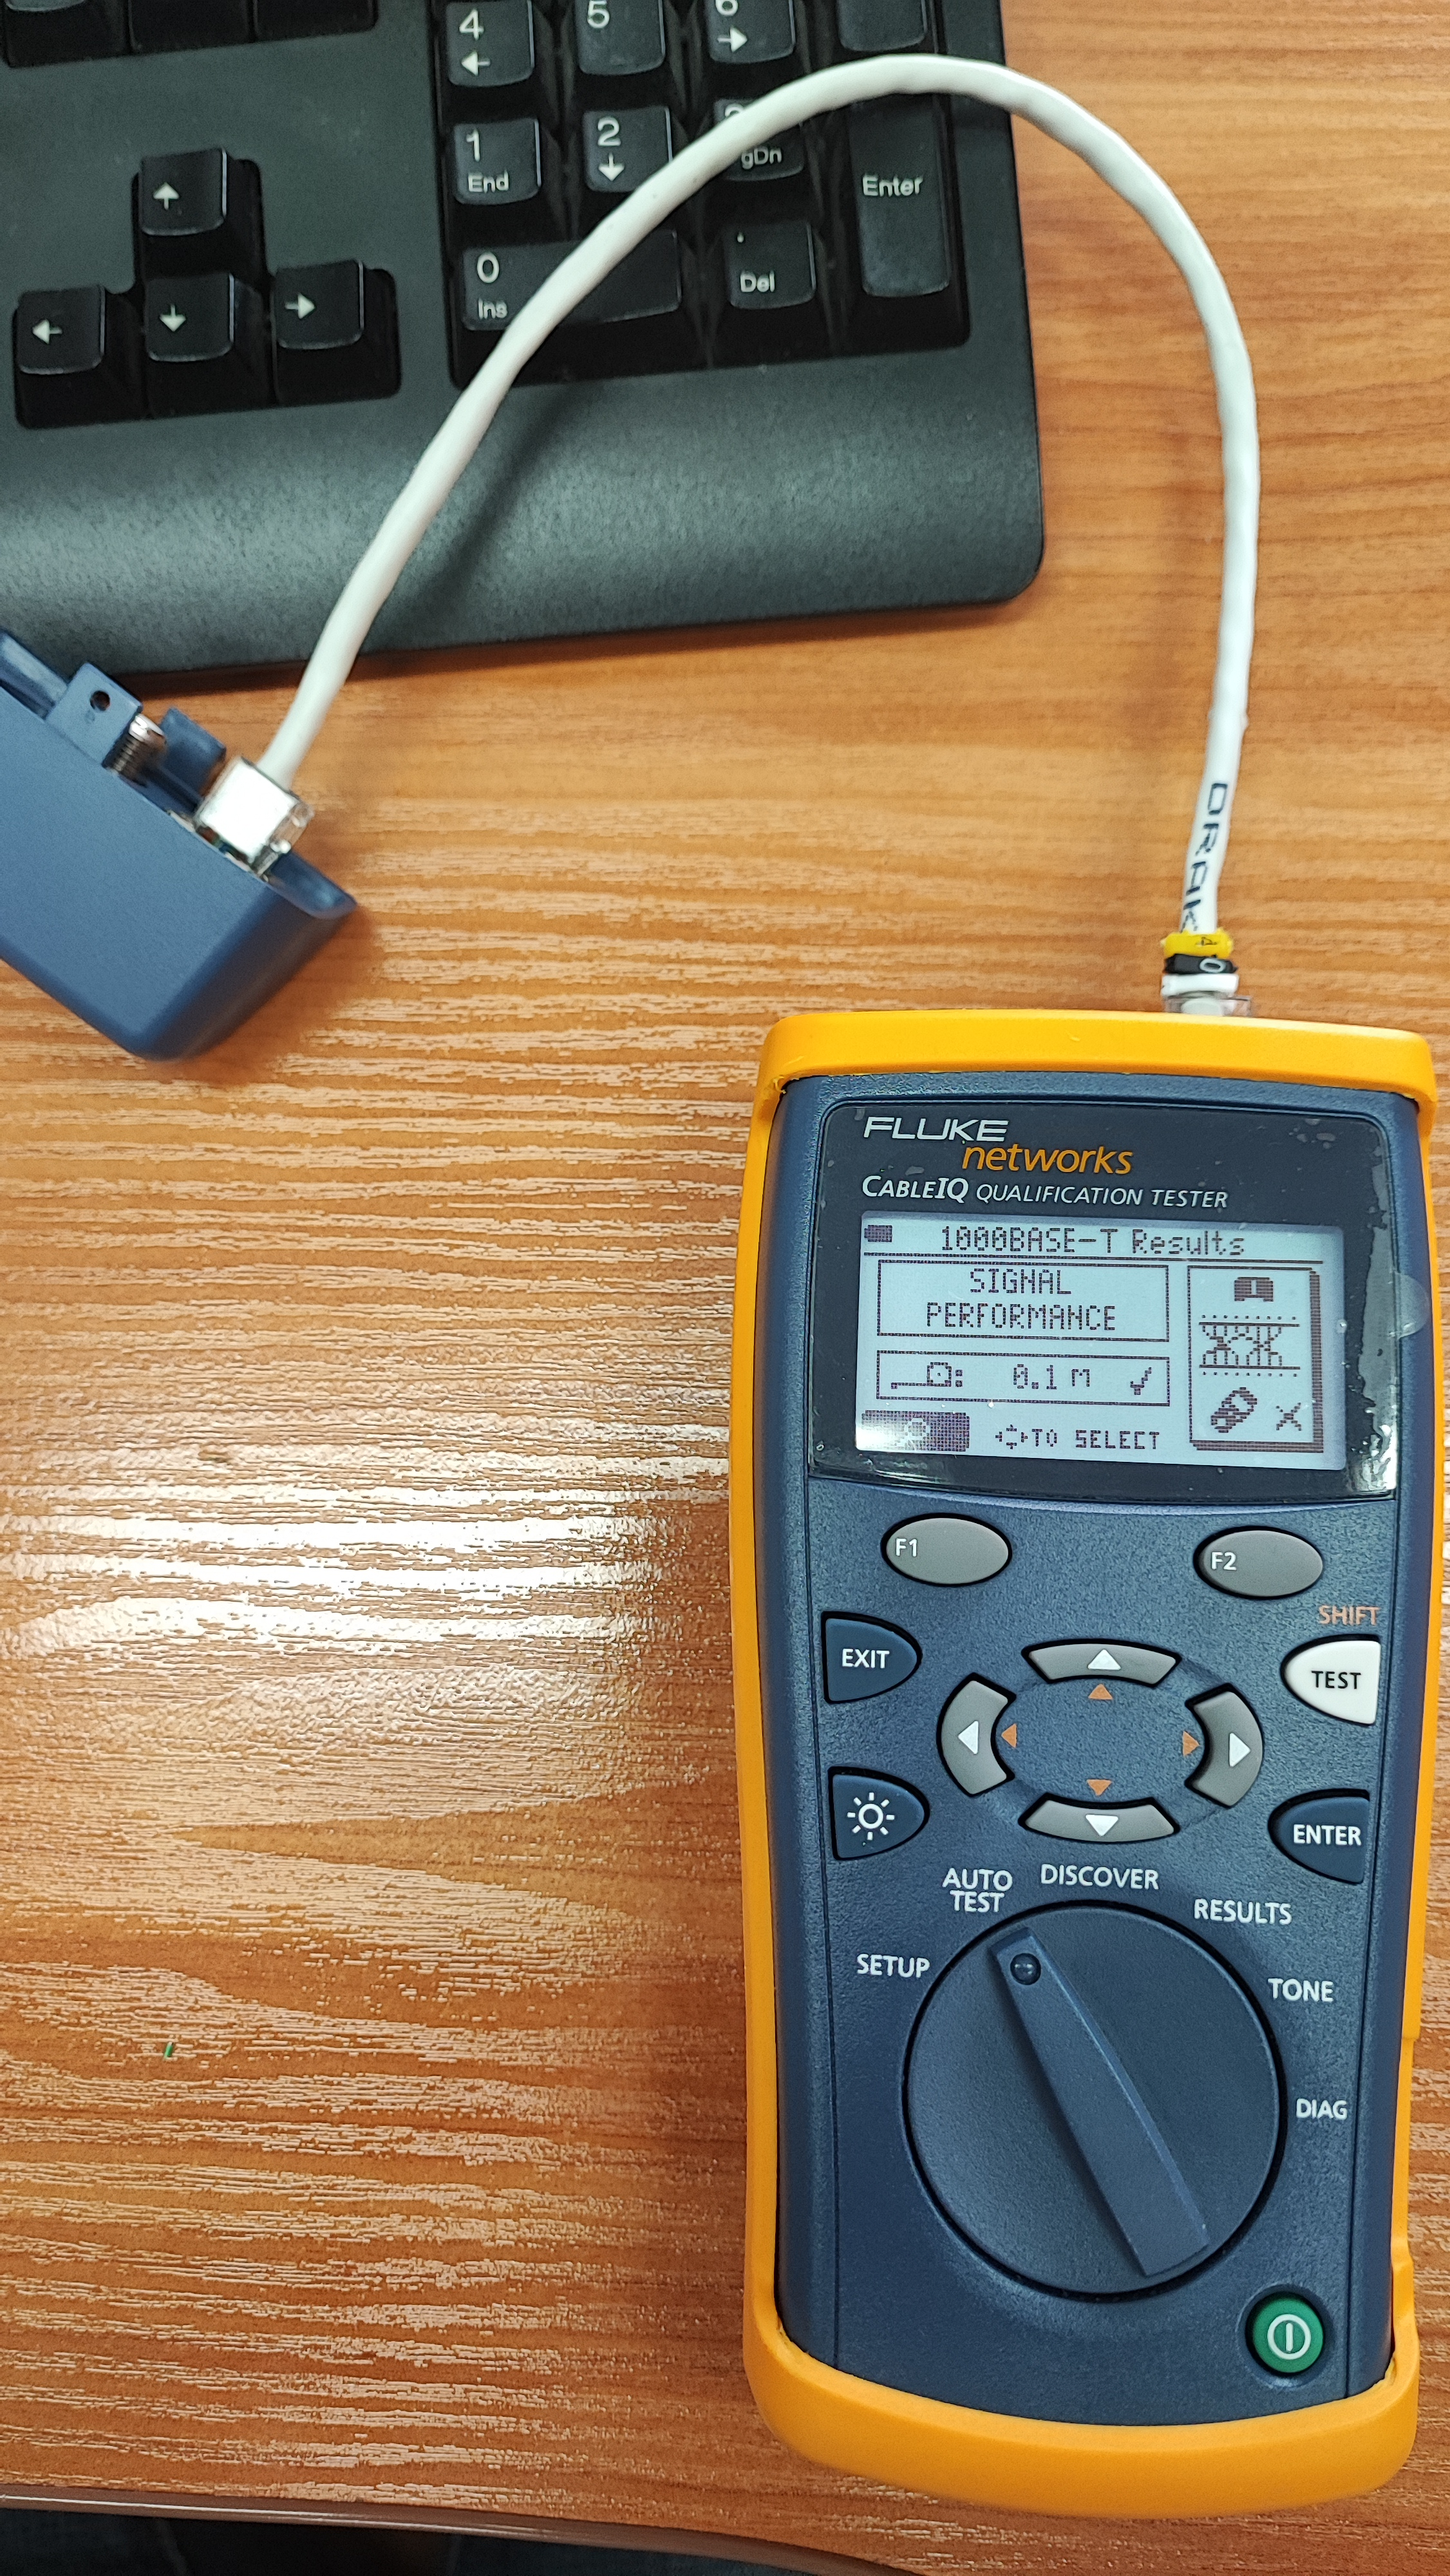
\includegraphics[width=0.63\textwidth]{fluke_wiring_fault_hot_tested.jpg}
\caption{Przypadek \textit{Wiring fault / Hot tested}}
\end{figure}

\begin{figure}[H]
\centering
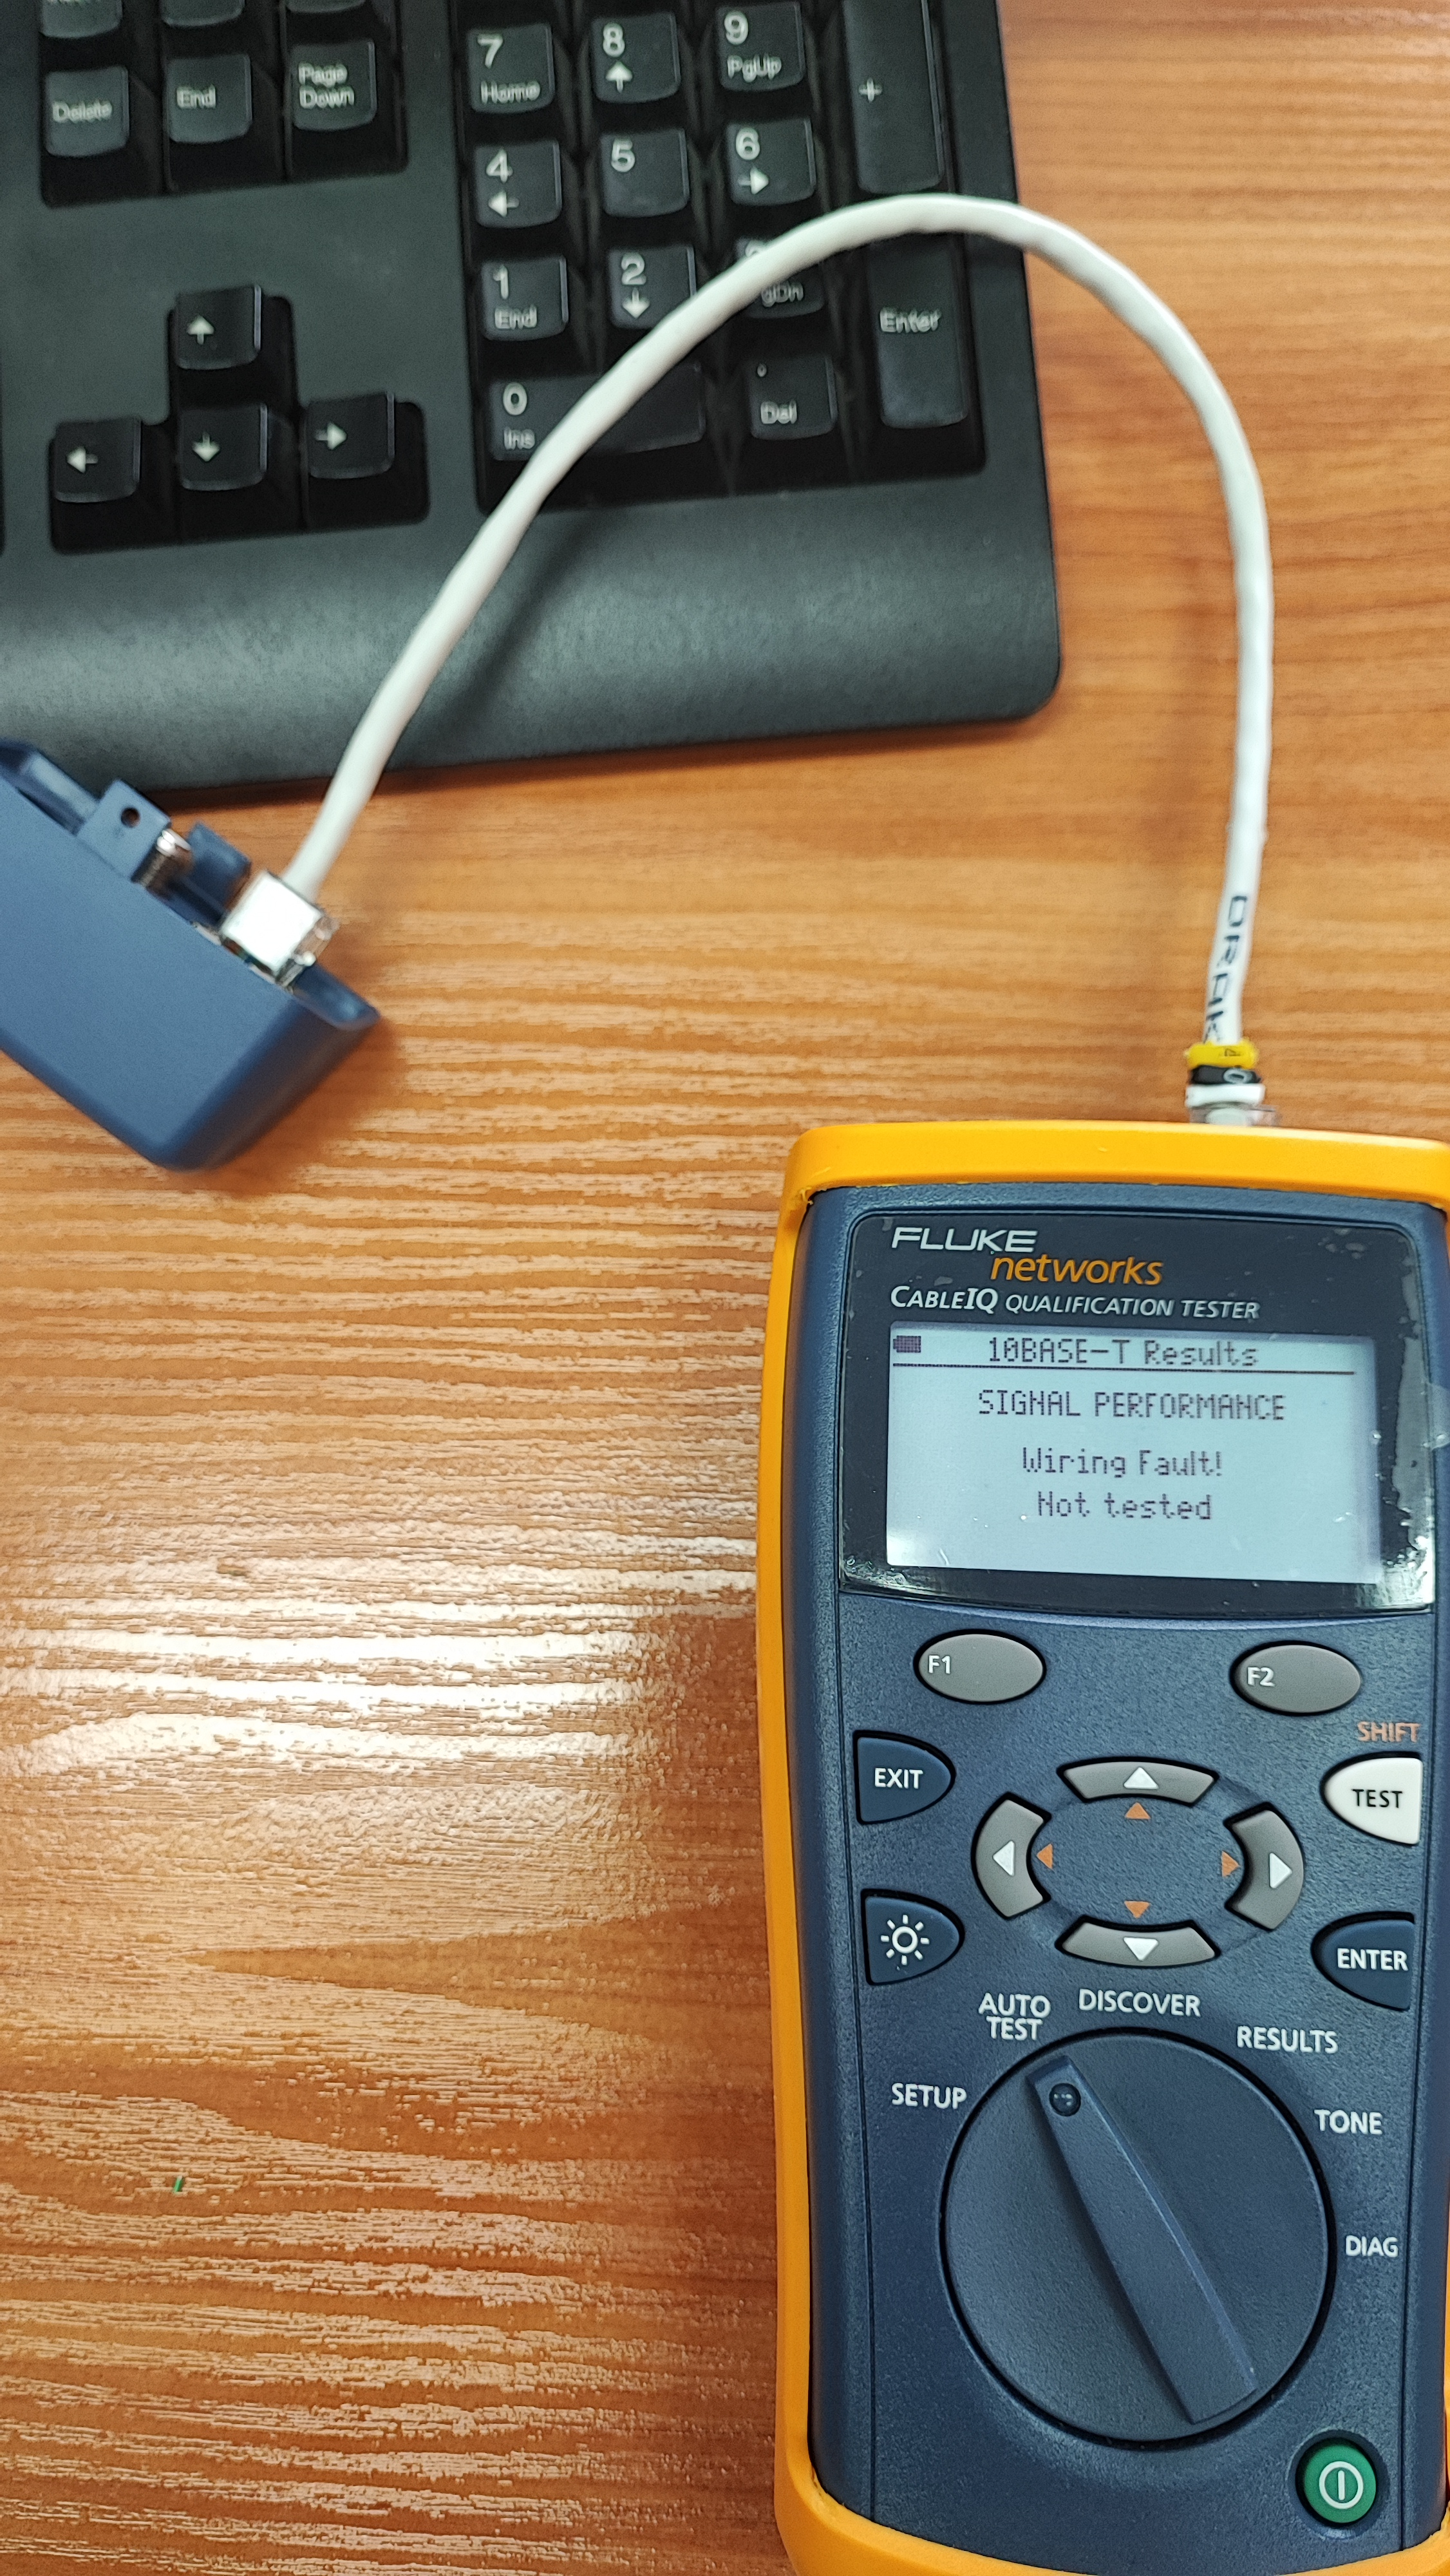
\includegraphics[width=0.63\textwidth]{fluke_wiring_fault_map.jpg}
\caption{Graficzna mapa połączeń z błędem -- skrzyżowanie par}
\end{figure}

\subsection{Wyniki testów patchpanelu}
Podczas testowania gniazd patchpanelu wykorzystaliśmy dwa patchcordy połączone z modułami master i remote. Na zdjęciach testera widzimy, że większość ścieżek zapewniała połączenia wszystkich ośmiu żył, natomiast błąd w jednej ścieżce był widoczny na ekranie jako \textit{Wiring fault}.

Miejscem pierwszego podejrzenia była końcówka patchcorda, dlatego po rozłączeniu ponownie sprawdziliśmy kolejność żył według T568A lub T568B. Kolejnym krokiem był test kabla między patchpanelem i gniazdem remote. Gdy problem pozostał po wymianie patchcorda, źródłem błędu był kabel stały, połączenie w tylnych gniazdach patchpanelu lub pominięta para.

\section{Analiza błędów i usterek}
\subsection{Rodzaje wykrytych nieprawidłowości}
\begin{enumerate}
  \item \textbf{Błąd kolejności żył.} Zaświadczają o tym skrzyżowania lub zamiany numerów pinów, np. 5--5 i 6--2.
  \item \textbf{Błąd połączenia par.} Kabel nie zachowuje par różnicowych 1--2, 3--6, 4--5 i 7--8.
  \item \textbf{Przerwa w przewodzie.} Tester nie uzyskiwał pełnego obwodu i wyświetlał brak jednej lub kilku żył.
  \item \textbf{Skrócenie/skrzyżowanie.} Dwie żyły były połączone z niewłaściwymi pinami; obok mapy przewodów pojawiał się stan \textit{Crossover}.
\end{enumerate}

\subsection{Przyczyny}
Najczęstsze przyczyny to:
\begin{itemize}
  \item zbyt mała lub zbyt duża głębokość odsłonięcia izolacji,
  \item żyły wsunięte do wtyczki w błędnej kolejności,
  \item zaciśnięcie kabla na żyłach zamiast na zewnętrznej izolacji,
  \item niepełne zaciśnięcie ostrza wtyczki,
  \item pomylenie pinów T568A z pinami T568B,
  \item brak oderwania starego fragmentu żyły z tylnej części patchpanelu,
  \item uszkodzenie izolacji lub przewodu,
  \item uszkodzony lub zanieczyszczony patchcord.
\end{itemize}

\subsection{Metoda usuwania błędu}
Po wykryciu błędu wymienialiśmy patchcord albo ponownie zaciśnęliśmy wtyczkę według tego samego standardu po obu stronach. Następnie porównywaliśmy mapę przewodów z tabelą par 12,36,45,78 i powtarzaliśmy pomiar. W razie niezgodności sprawdzaliśmy miejsce uszkodzenia etapami: patchcordem, patchpanelem i połączeniami w tylnych gniazdach.

\section{Dokumentacja filmów}
W folderze \texttt{dane} znajduje się sześć nagrań demonstrujących testy kabli i patchpanelu. Poniżej umieściliśmy reprezentatywne klatki pozyskane z nagrań.

\begin{figure}[H]
\centering
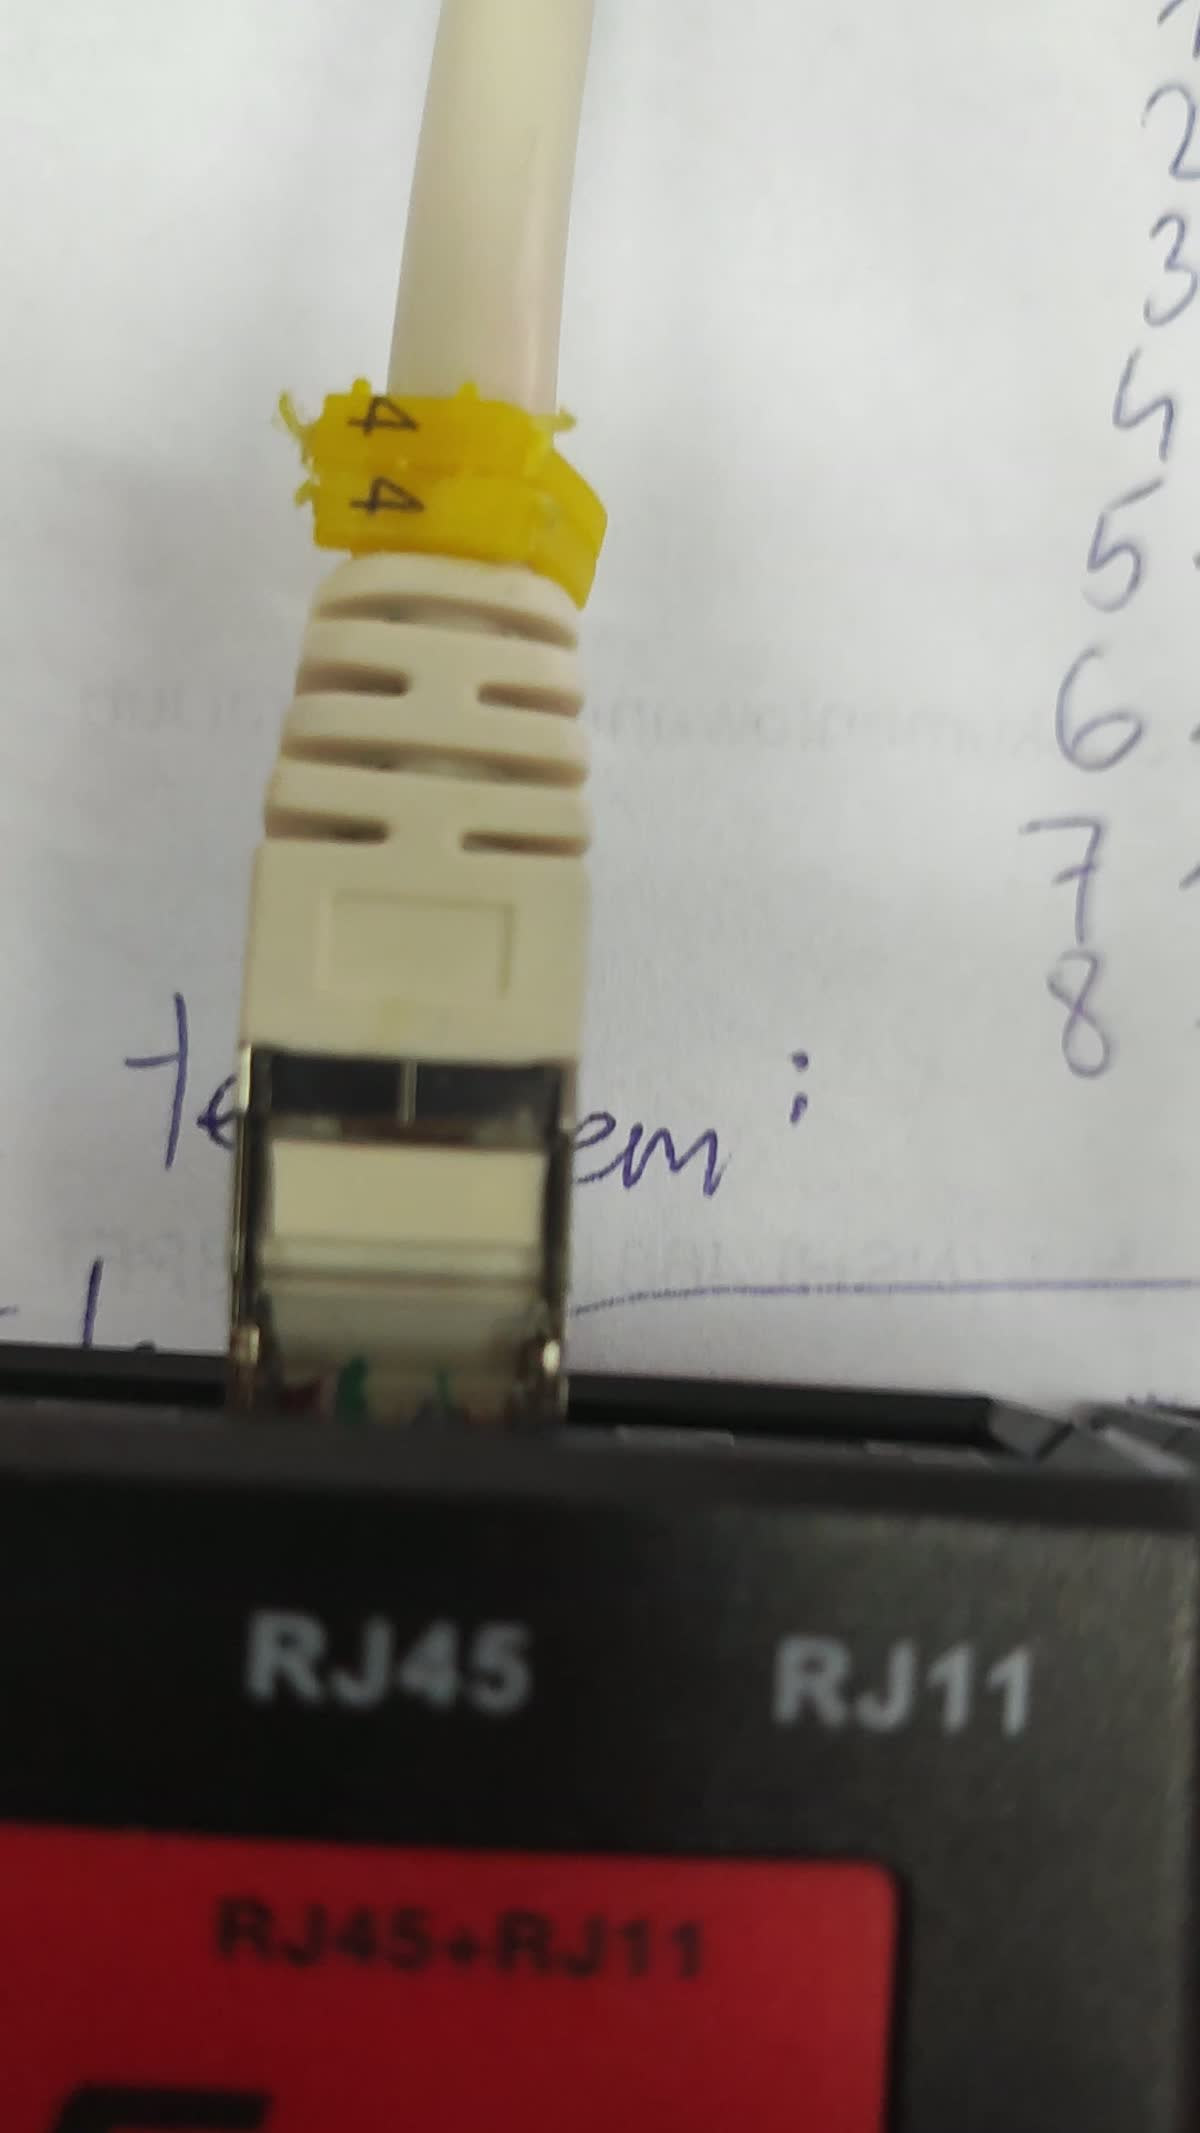
\includegraphics[width=0.75\textwidth]{klatki/patchpanel_module_test_frame.jpg}
\caption{Nagranie \texttt{patchpanel\_module\_test.mp4} -- test modułu po stronie patchpanelu}
\end{figure}

\begin{figure}[H]
\centering
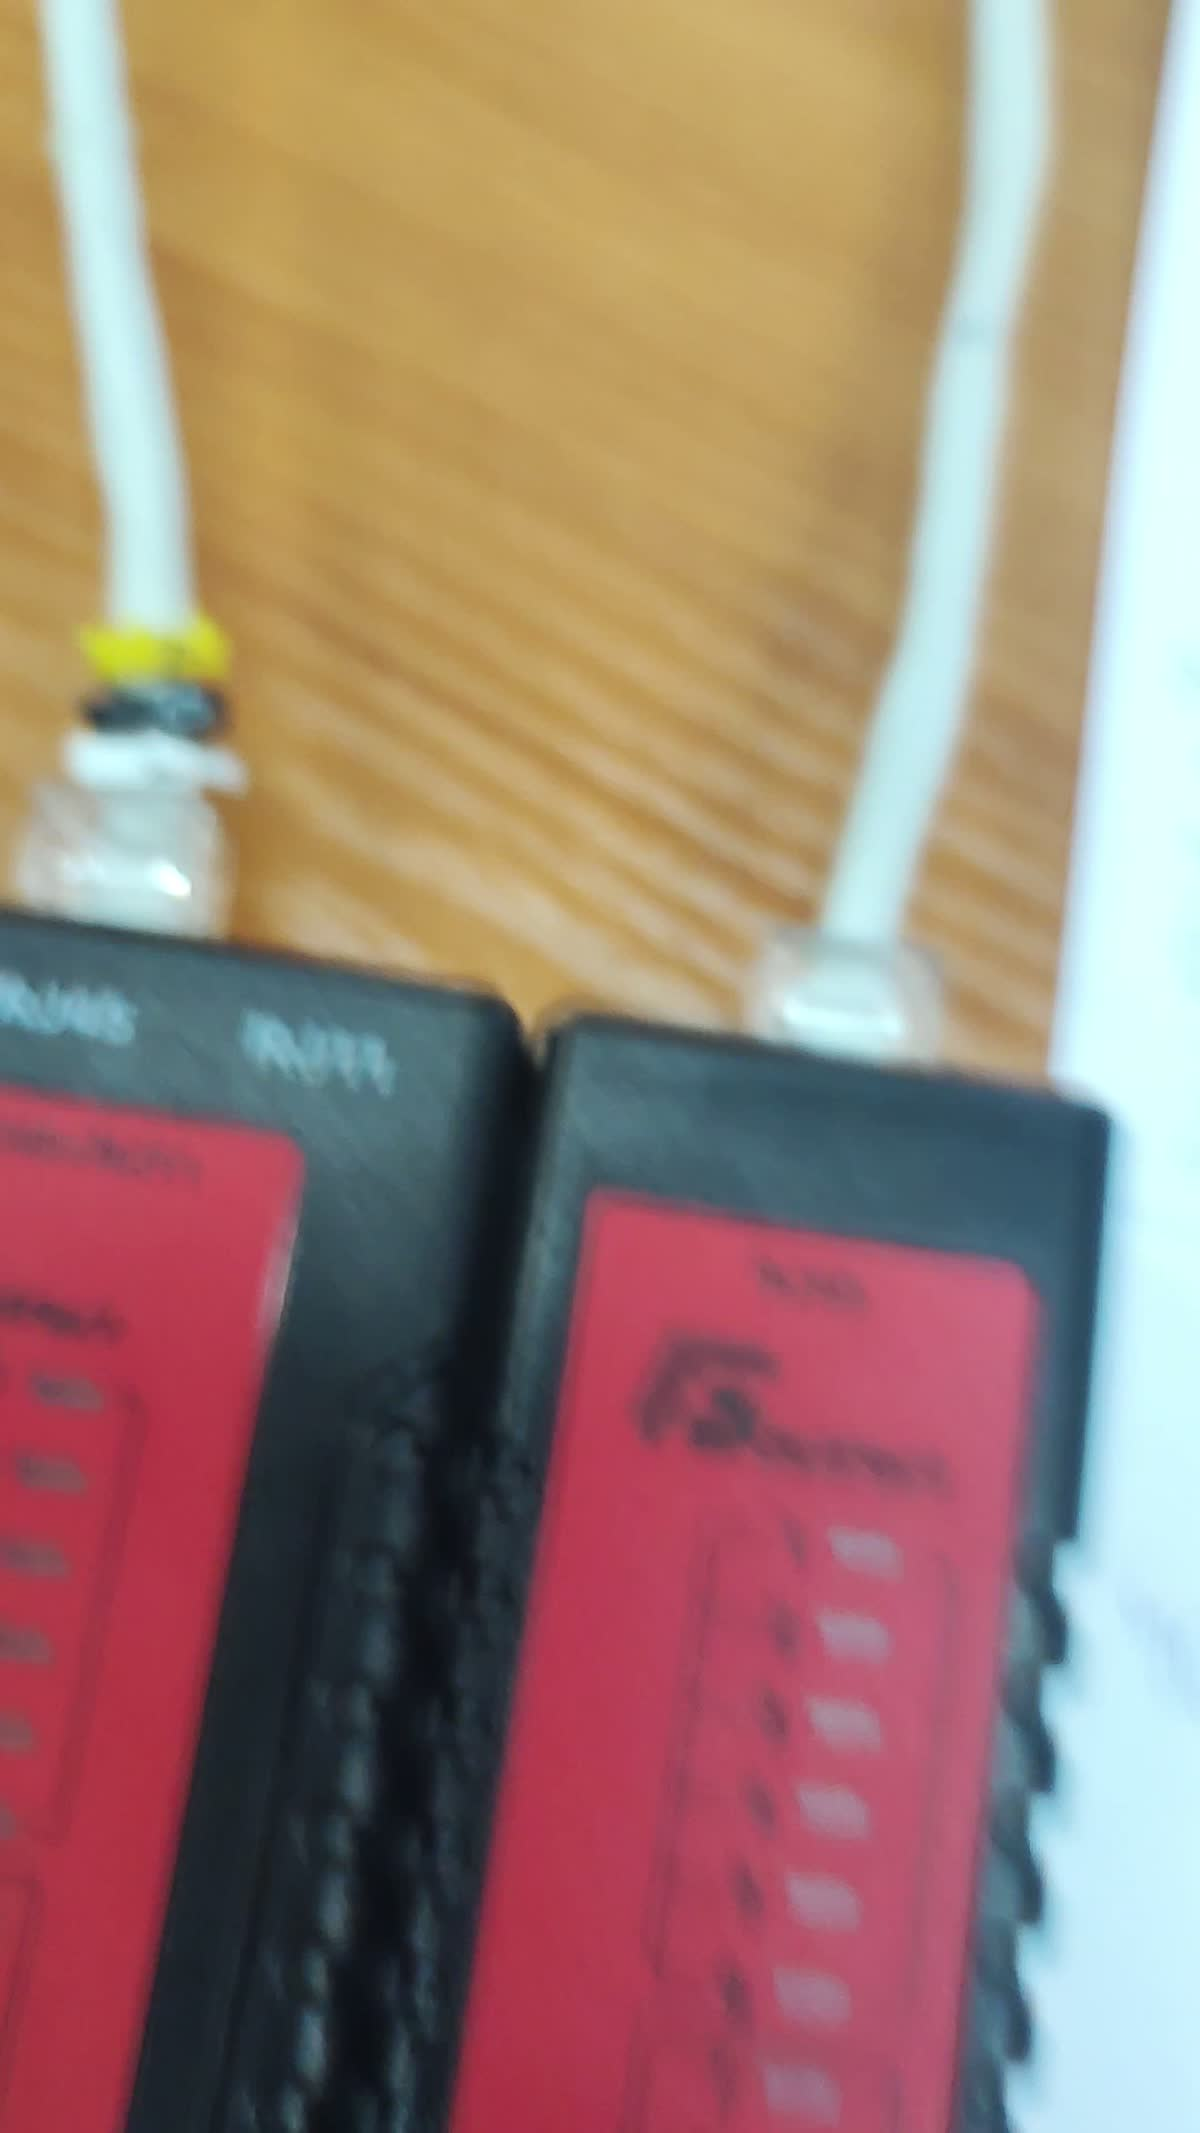
\includegraphics[width=0.75\textwidth]{klatki/patchpanel_ports_sequence_frame.jpg}
\caption{Nagranie \texttt{patchpanel\_ports\_sequence.mp4} -- sprawdzanie kolejnych gniazd}
\end{figure}

\begin{figure}[H]
\centering
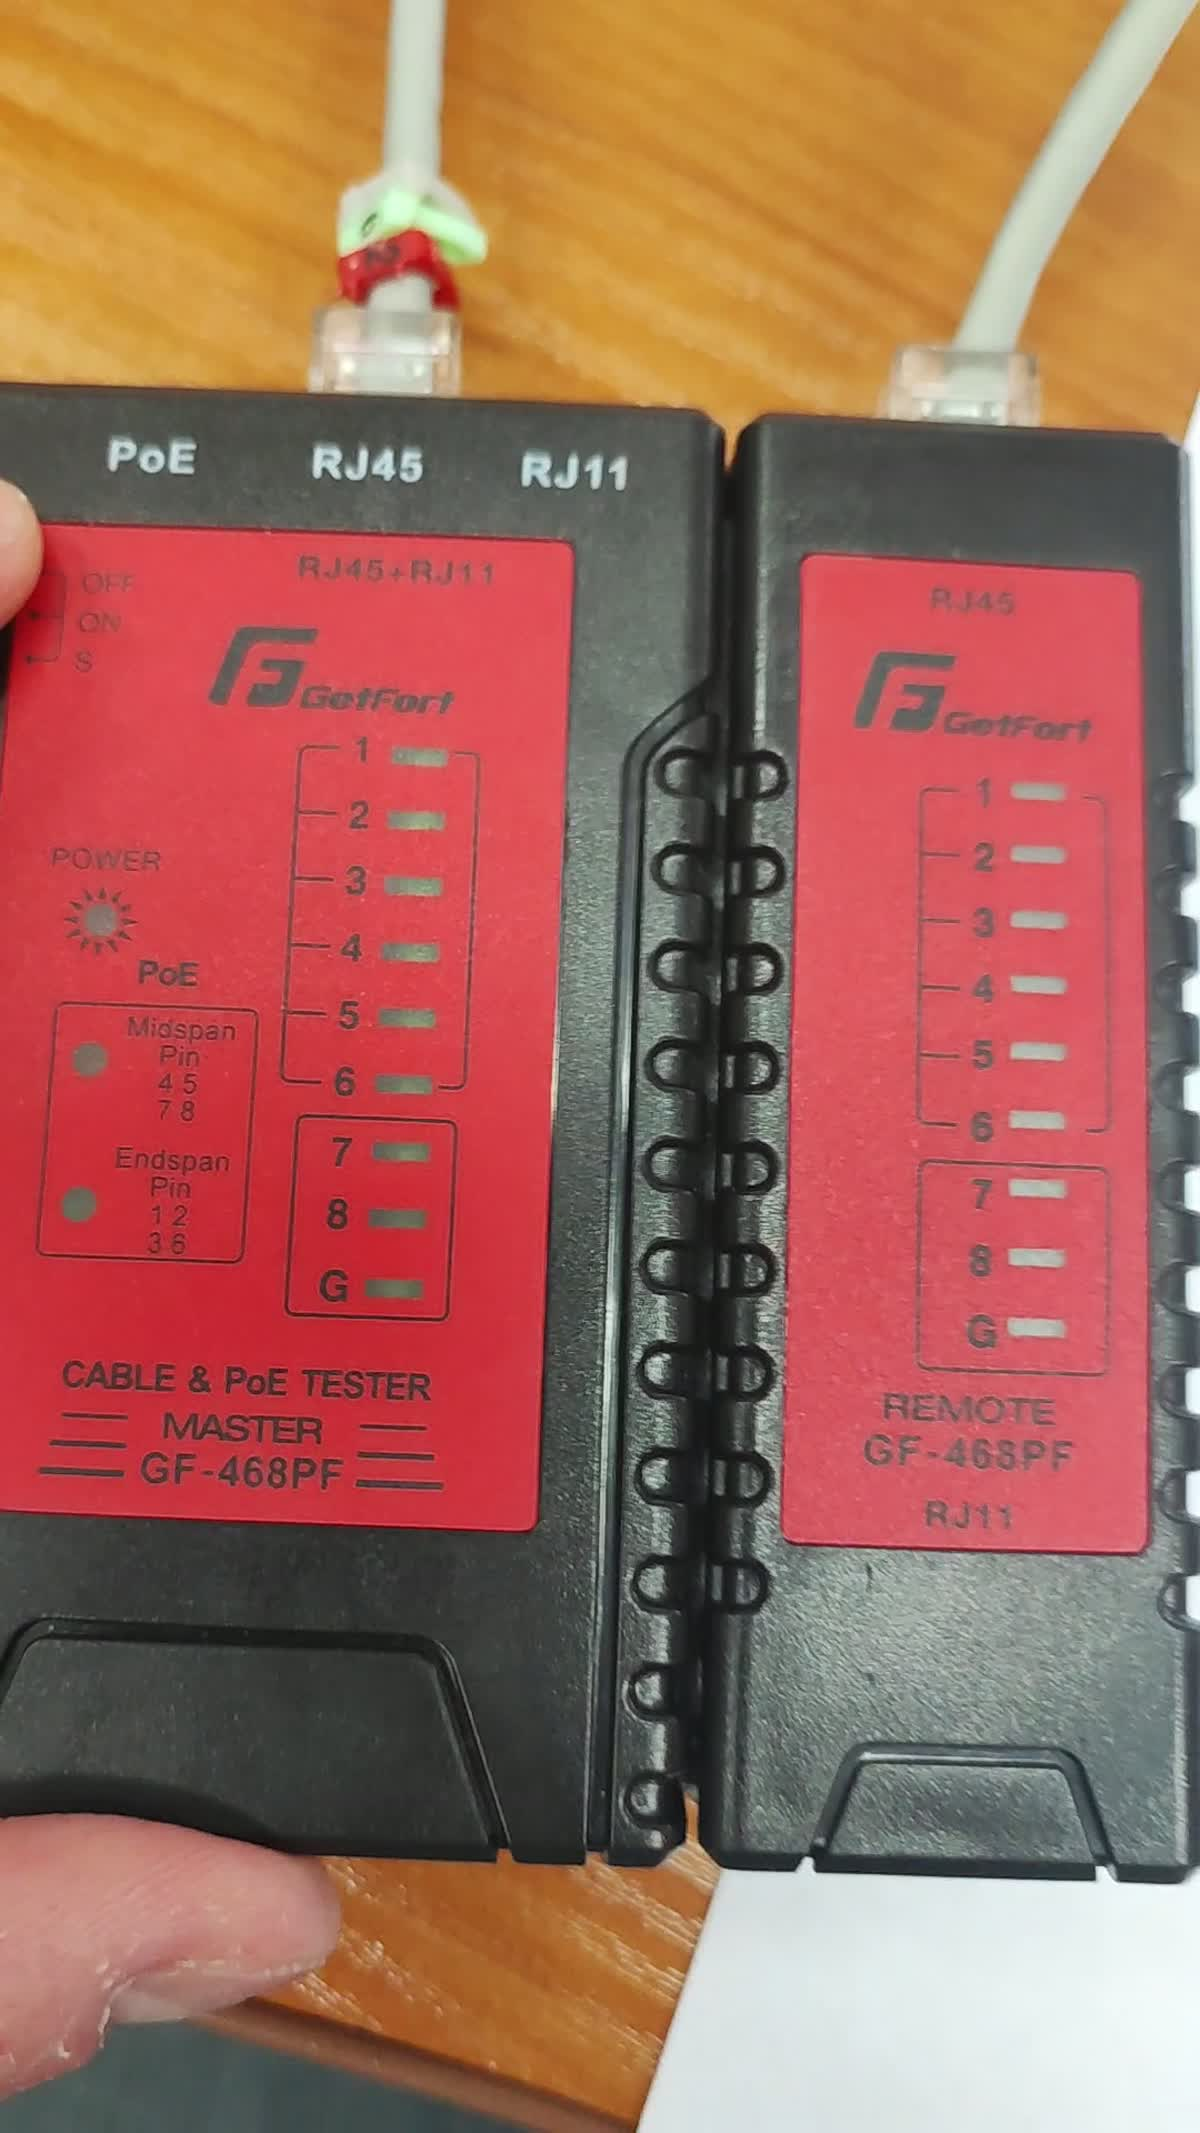
\includegraphics[width=0.75\textwidth]{klatki/patchpanel_wire_sequence_frame.jpg}
\caption{Nagranie \texttt{patchpanel\_wire\_sequence.mp4} -- test połączenia i kolejności żył}
\end{figure}

\begin{figure}[H]
\centering
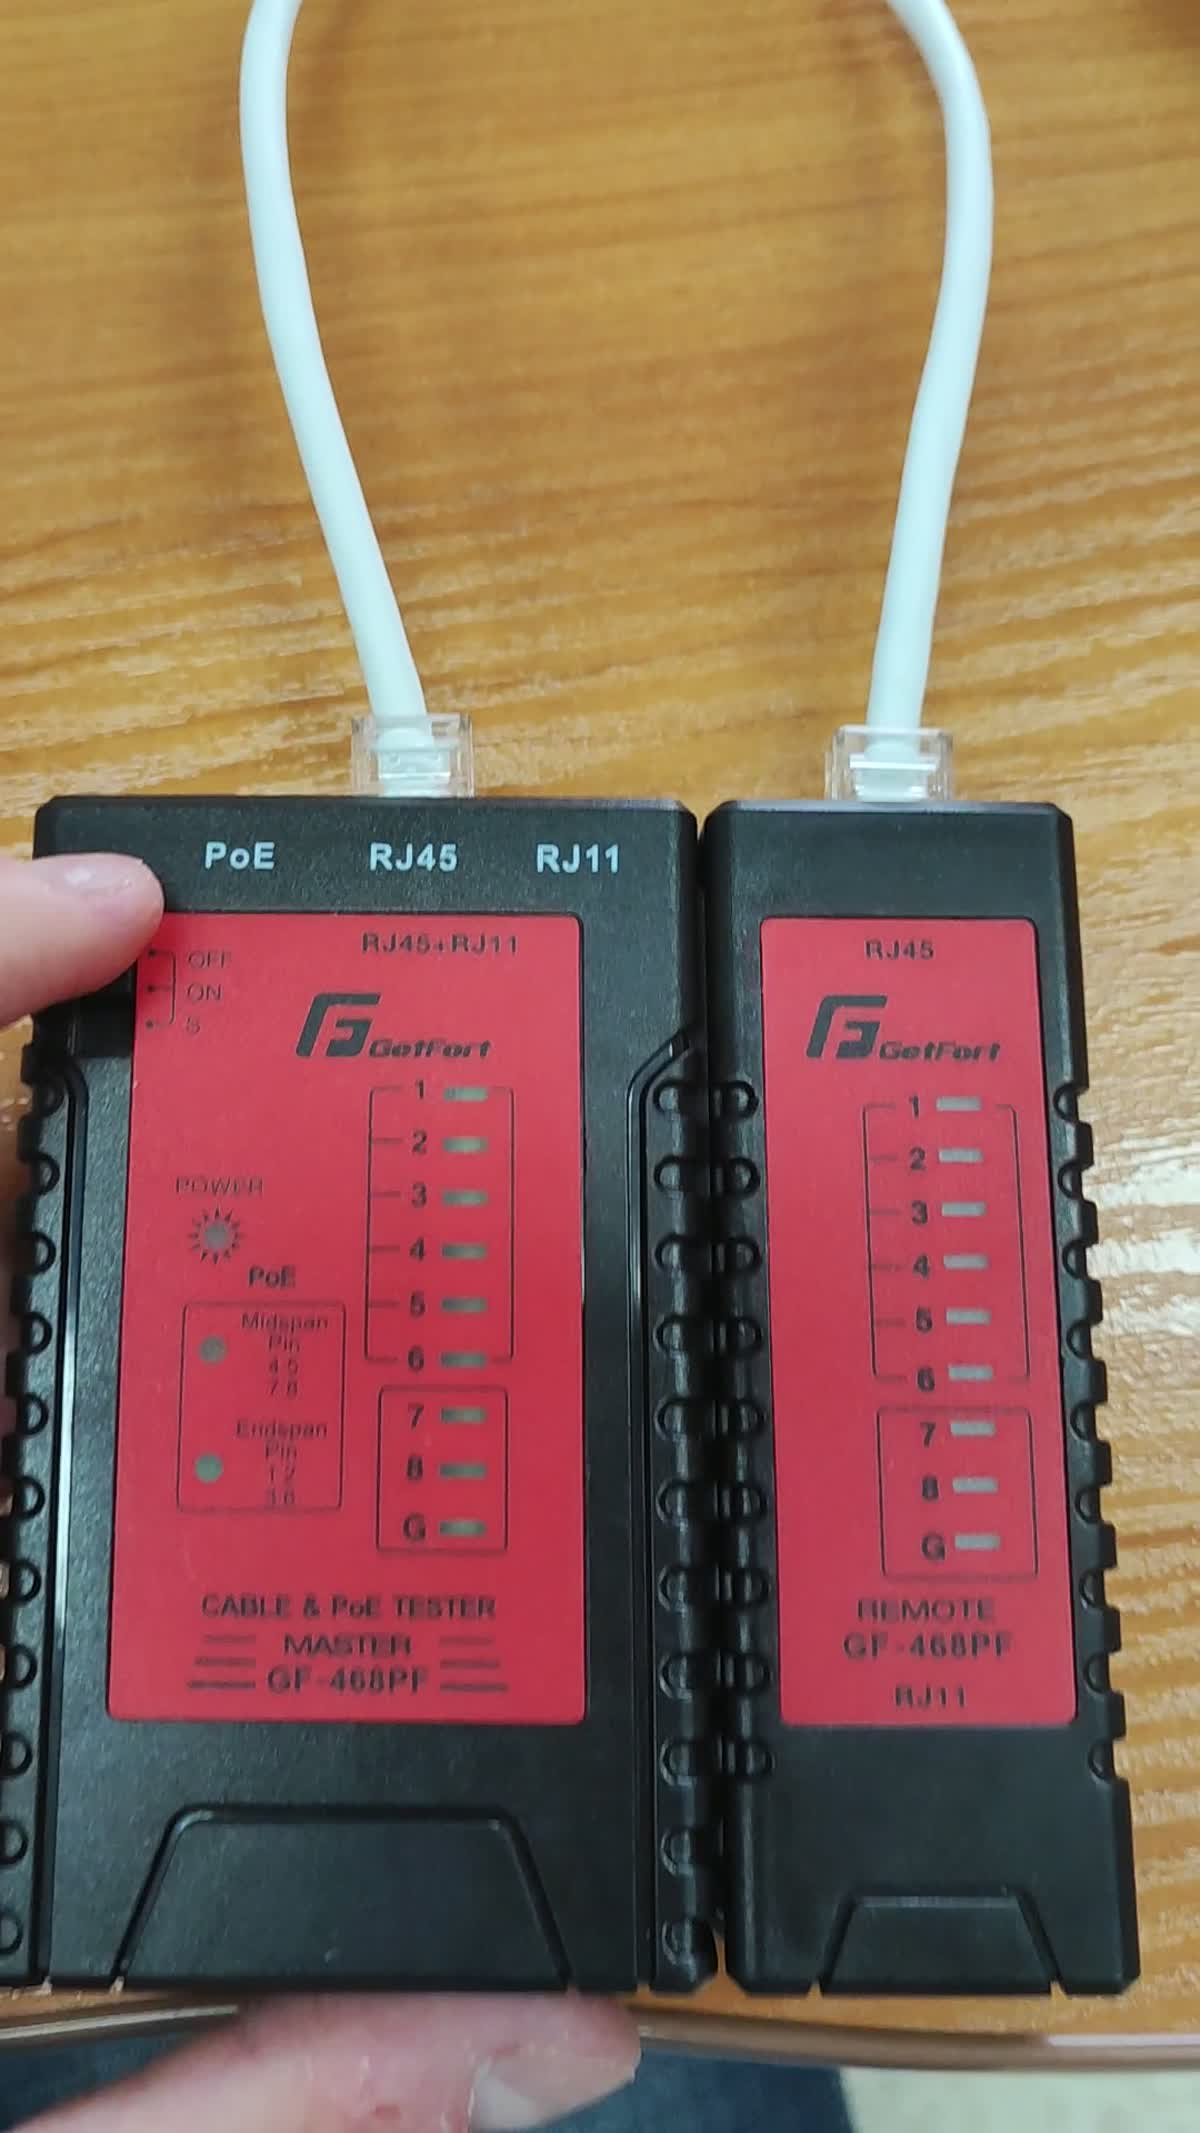
\includegraphics[width=0.75\textwidth]{klatki/patchpanel_test_results_frame.jpg}
\caption{Nagranie \texttt{patchpanel\_test\_results.mp4} -- dokumentacja wyników testu}
\end{figure}

\begin{figure}[H]
\centering
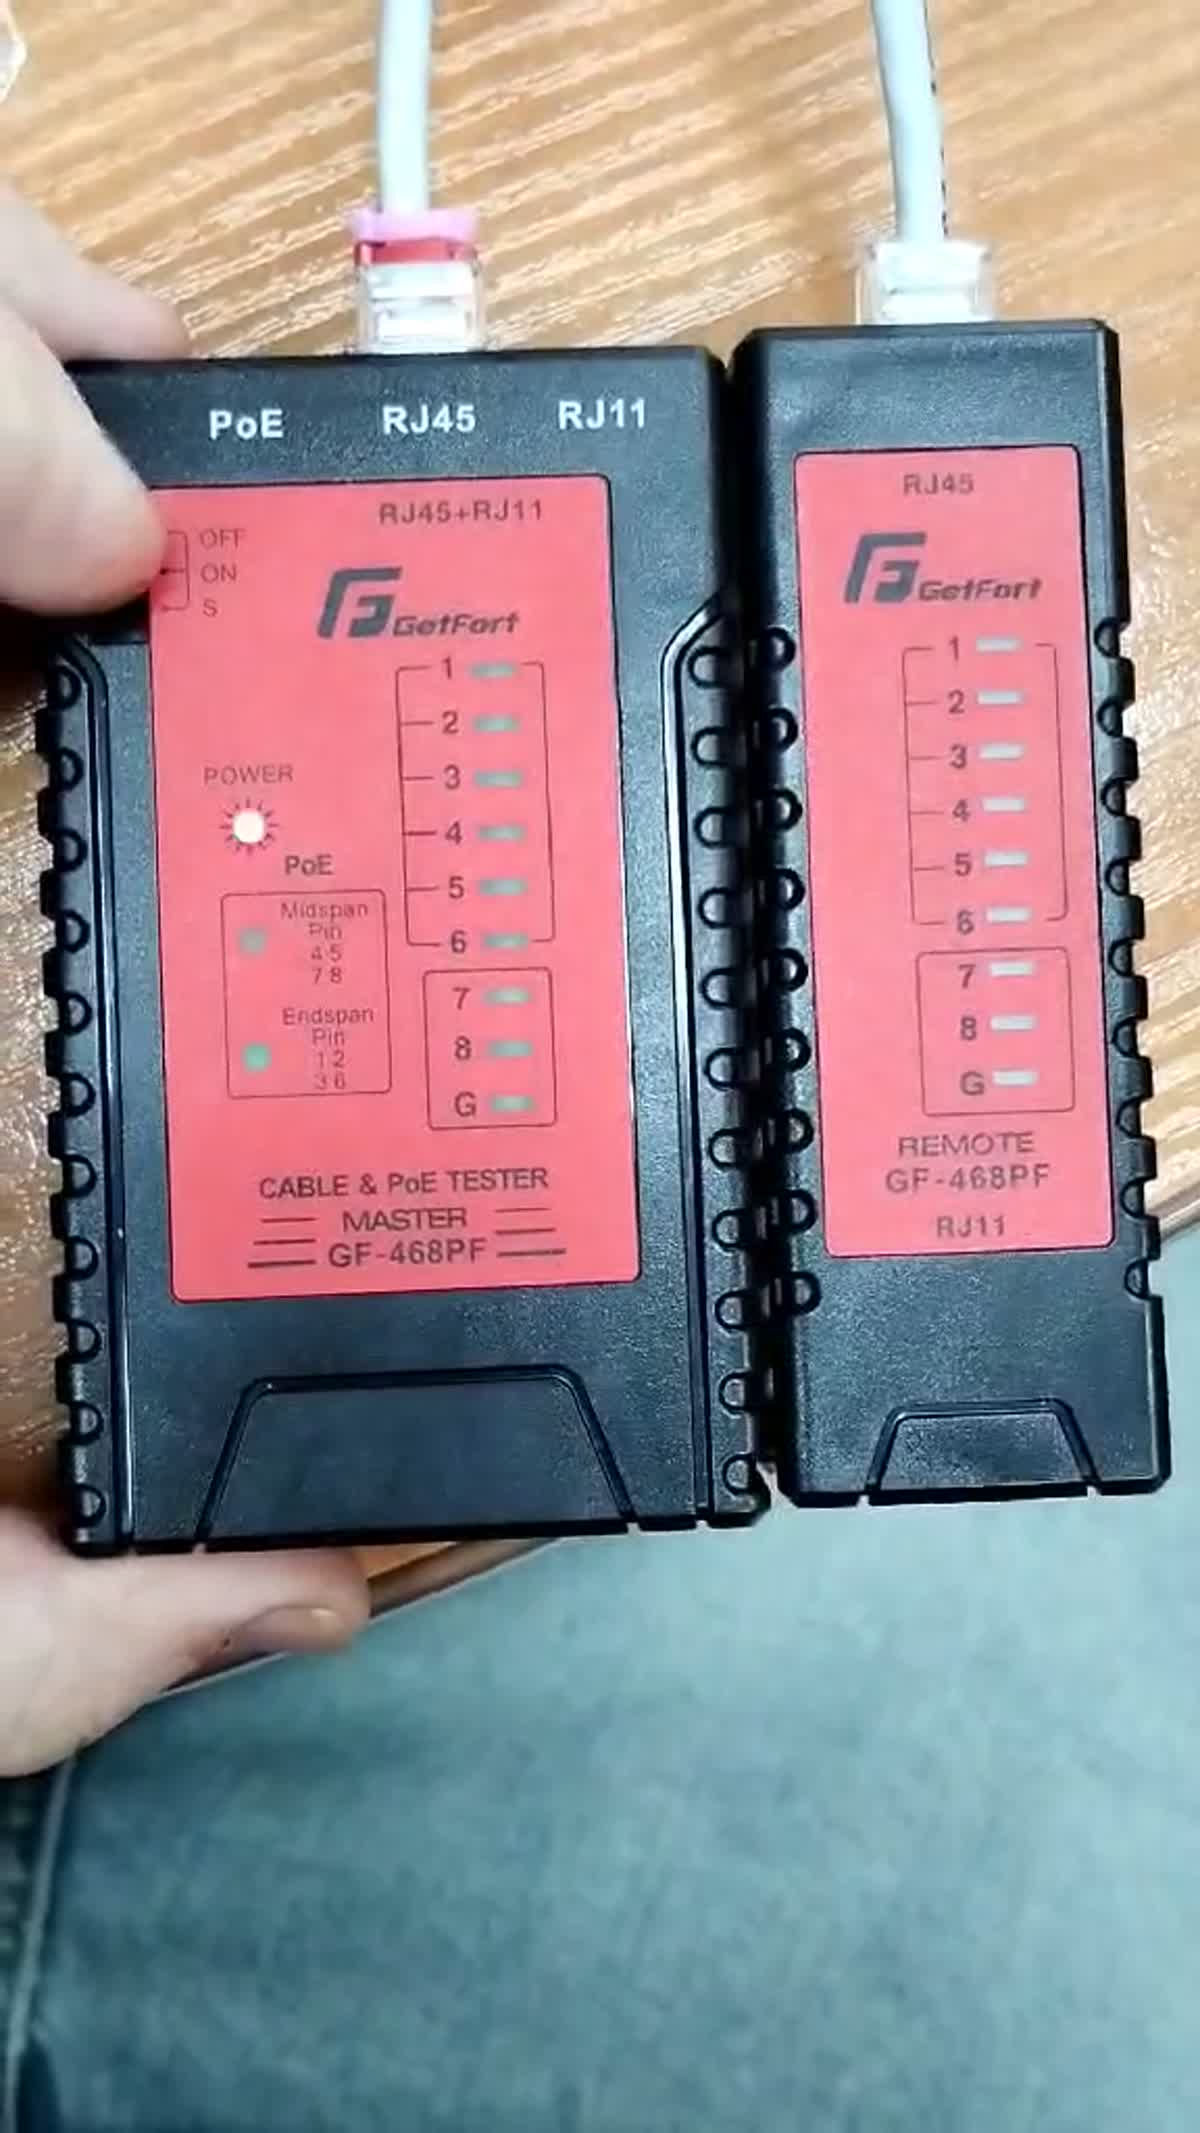
\includegraphics[width=0.75\textwidth]{klatki/patchcord_test_pairs_frame.jpg}
\caption{Nagranie \texttt{patchcord\_test\_pairs.mp4} -- test par i wtyczek}
\end{figure}

\begin{figure}[H]
\centering
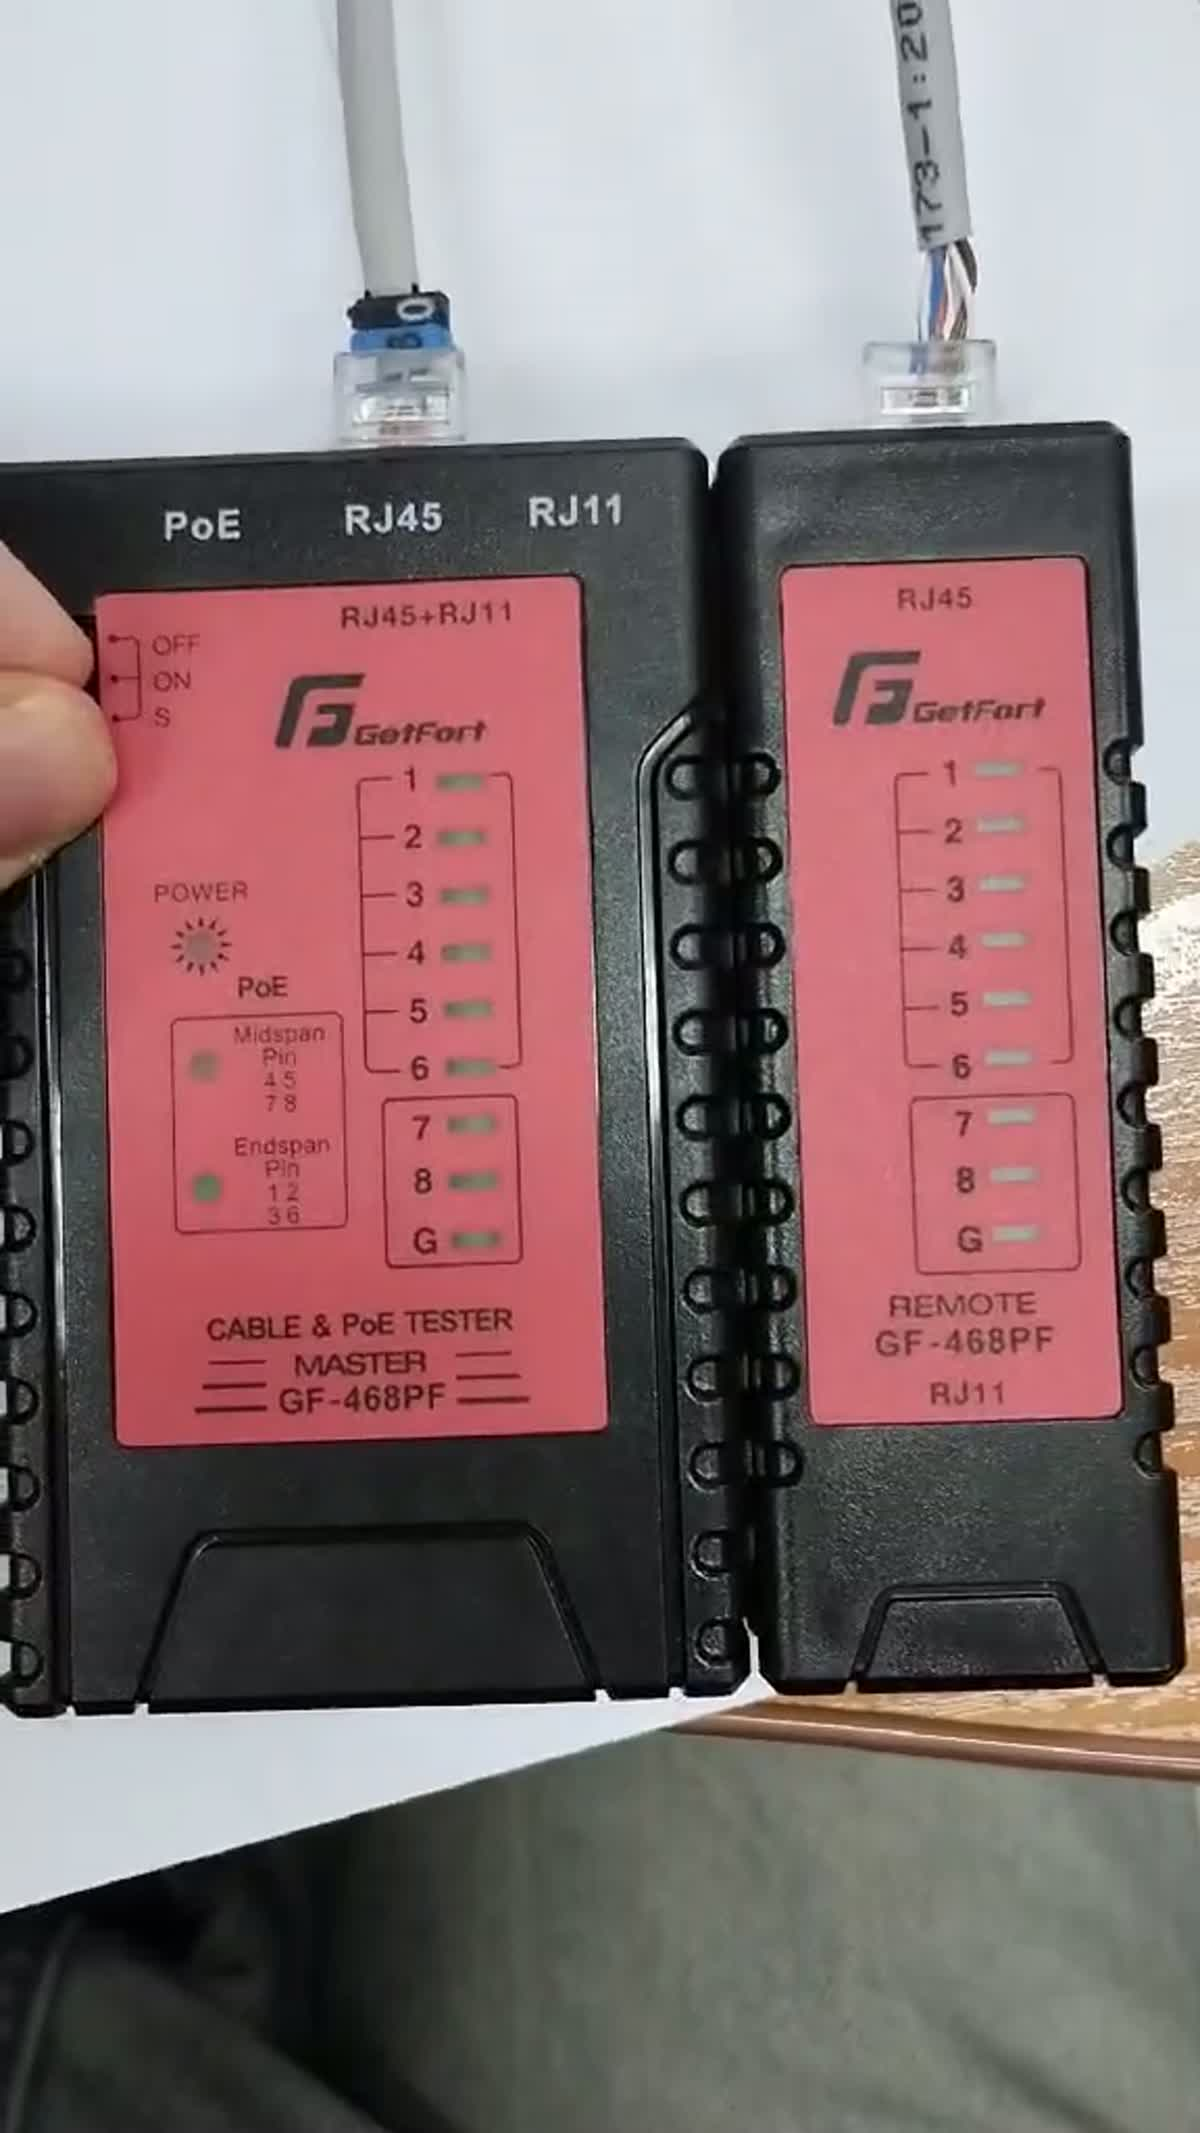
\includegraphics[width=0.75\textwidth]{klatki/patchpanel_test_path_frame.jpg}
\caption{Nagranie \texttt{patchpanel\_test\_path.mp4} -- test ścieżki w patchpanelu}
\end{figure}

\section{Opracowanie wyników}
Wszystkie poprawnie zaciśnięte i jednolite kable wykazywały:
\begin{itemize}
  \item zachowanie mapy przewodów 1--1, 2--2, 3--3, 4--4, 5--5, 6--6, 7--7 i 8--8 dla kabla prostego,
  \item poprawne pary 1--2, 3--6, 4--5 i 7--8,
  \item długości 0,1--0,2 m dla badanych patchcordów,
  \item kwalifikację na 1000BASE-T dla ścieżki nieposiadającej błędu,
  \item poprawne działanie trzech standardów Ethernet dla skrótów 10BASE-T, 100BASE-TX i 1000BASE-T.
\end{itemize}

Wystąpiły również testy z błędem \textit{Wiring fault} oraz mapą skrzyżowań. Błędy były wynikiem nieprawidłowości kolejności żył, złego zaciśnięcia lub pomieszania kabla z zakończeniem T568A i T568B.

\section{Wnioski}
\begin{enumerate}
  \item Prawidłowa kolejność żył i zachowanie par różnicowych są warunkami działania Ethernetu po miedzi.
  \item Kabel prosty musi być zaciśnięty według jednego konsekwentnie zastosowanego schematu po obu stronach. Mieszanie T568A i T568B tworzy kabel krzyżowy lub połączenie niezgodne z zamierzonym zastosowaniem.
  \item Tester podstawowy i CableIQ wykryły poprawne połączenia i usterki, ale kwalifikator dostarczał większe informacje: mapę par, długość i standard Ethernet.
  \item Krótkie patchcordy o długości około 0,1--0,2 m spełniały warunki połączeń 10/100/1000 Mb/s.
  \item \textit{Wiring fault}, przerwanie lub crossover należy usunąć przed podłączeniem ścieżki do switcha, punktu dostępowego lub zasilacza PoE.
  \item Budowa ścieżki w patchpanelu wymaga etykietowania kabli i osobnego testu każdego etapu: kabla, patchcorda, gniazda i urządzenia aktywnego.
  \item Najważniejszymi czynnikami jakościowym jest powtarzalny proces zaciśnięcia, płytkie i jednorodne ułożenie żył oraz dokładna kontrola po zaciśnięciu.
\end{enumerate}

\section{Pełna dokumentacja zdjęć i nagrań}
\subsection{Zdjęcia numerowane kamerą}
Poniżej wszystkie fotografie \texttt{IMG\_20261110\_*.jpg} są przedstawione osobno, aby wyniki na ekranach testera były czytelne.
\clearpage

\begin{figure}[H]
\centering
\begin{minipage}{0.48\textwidth}
\centering
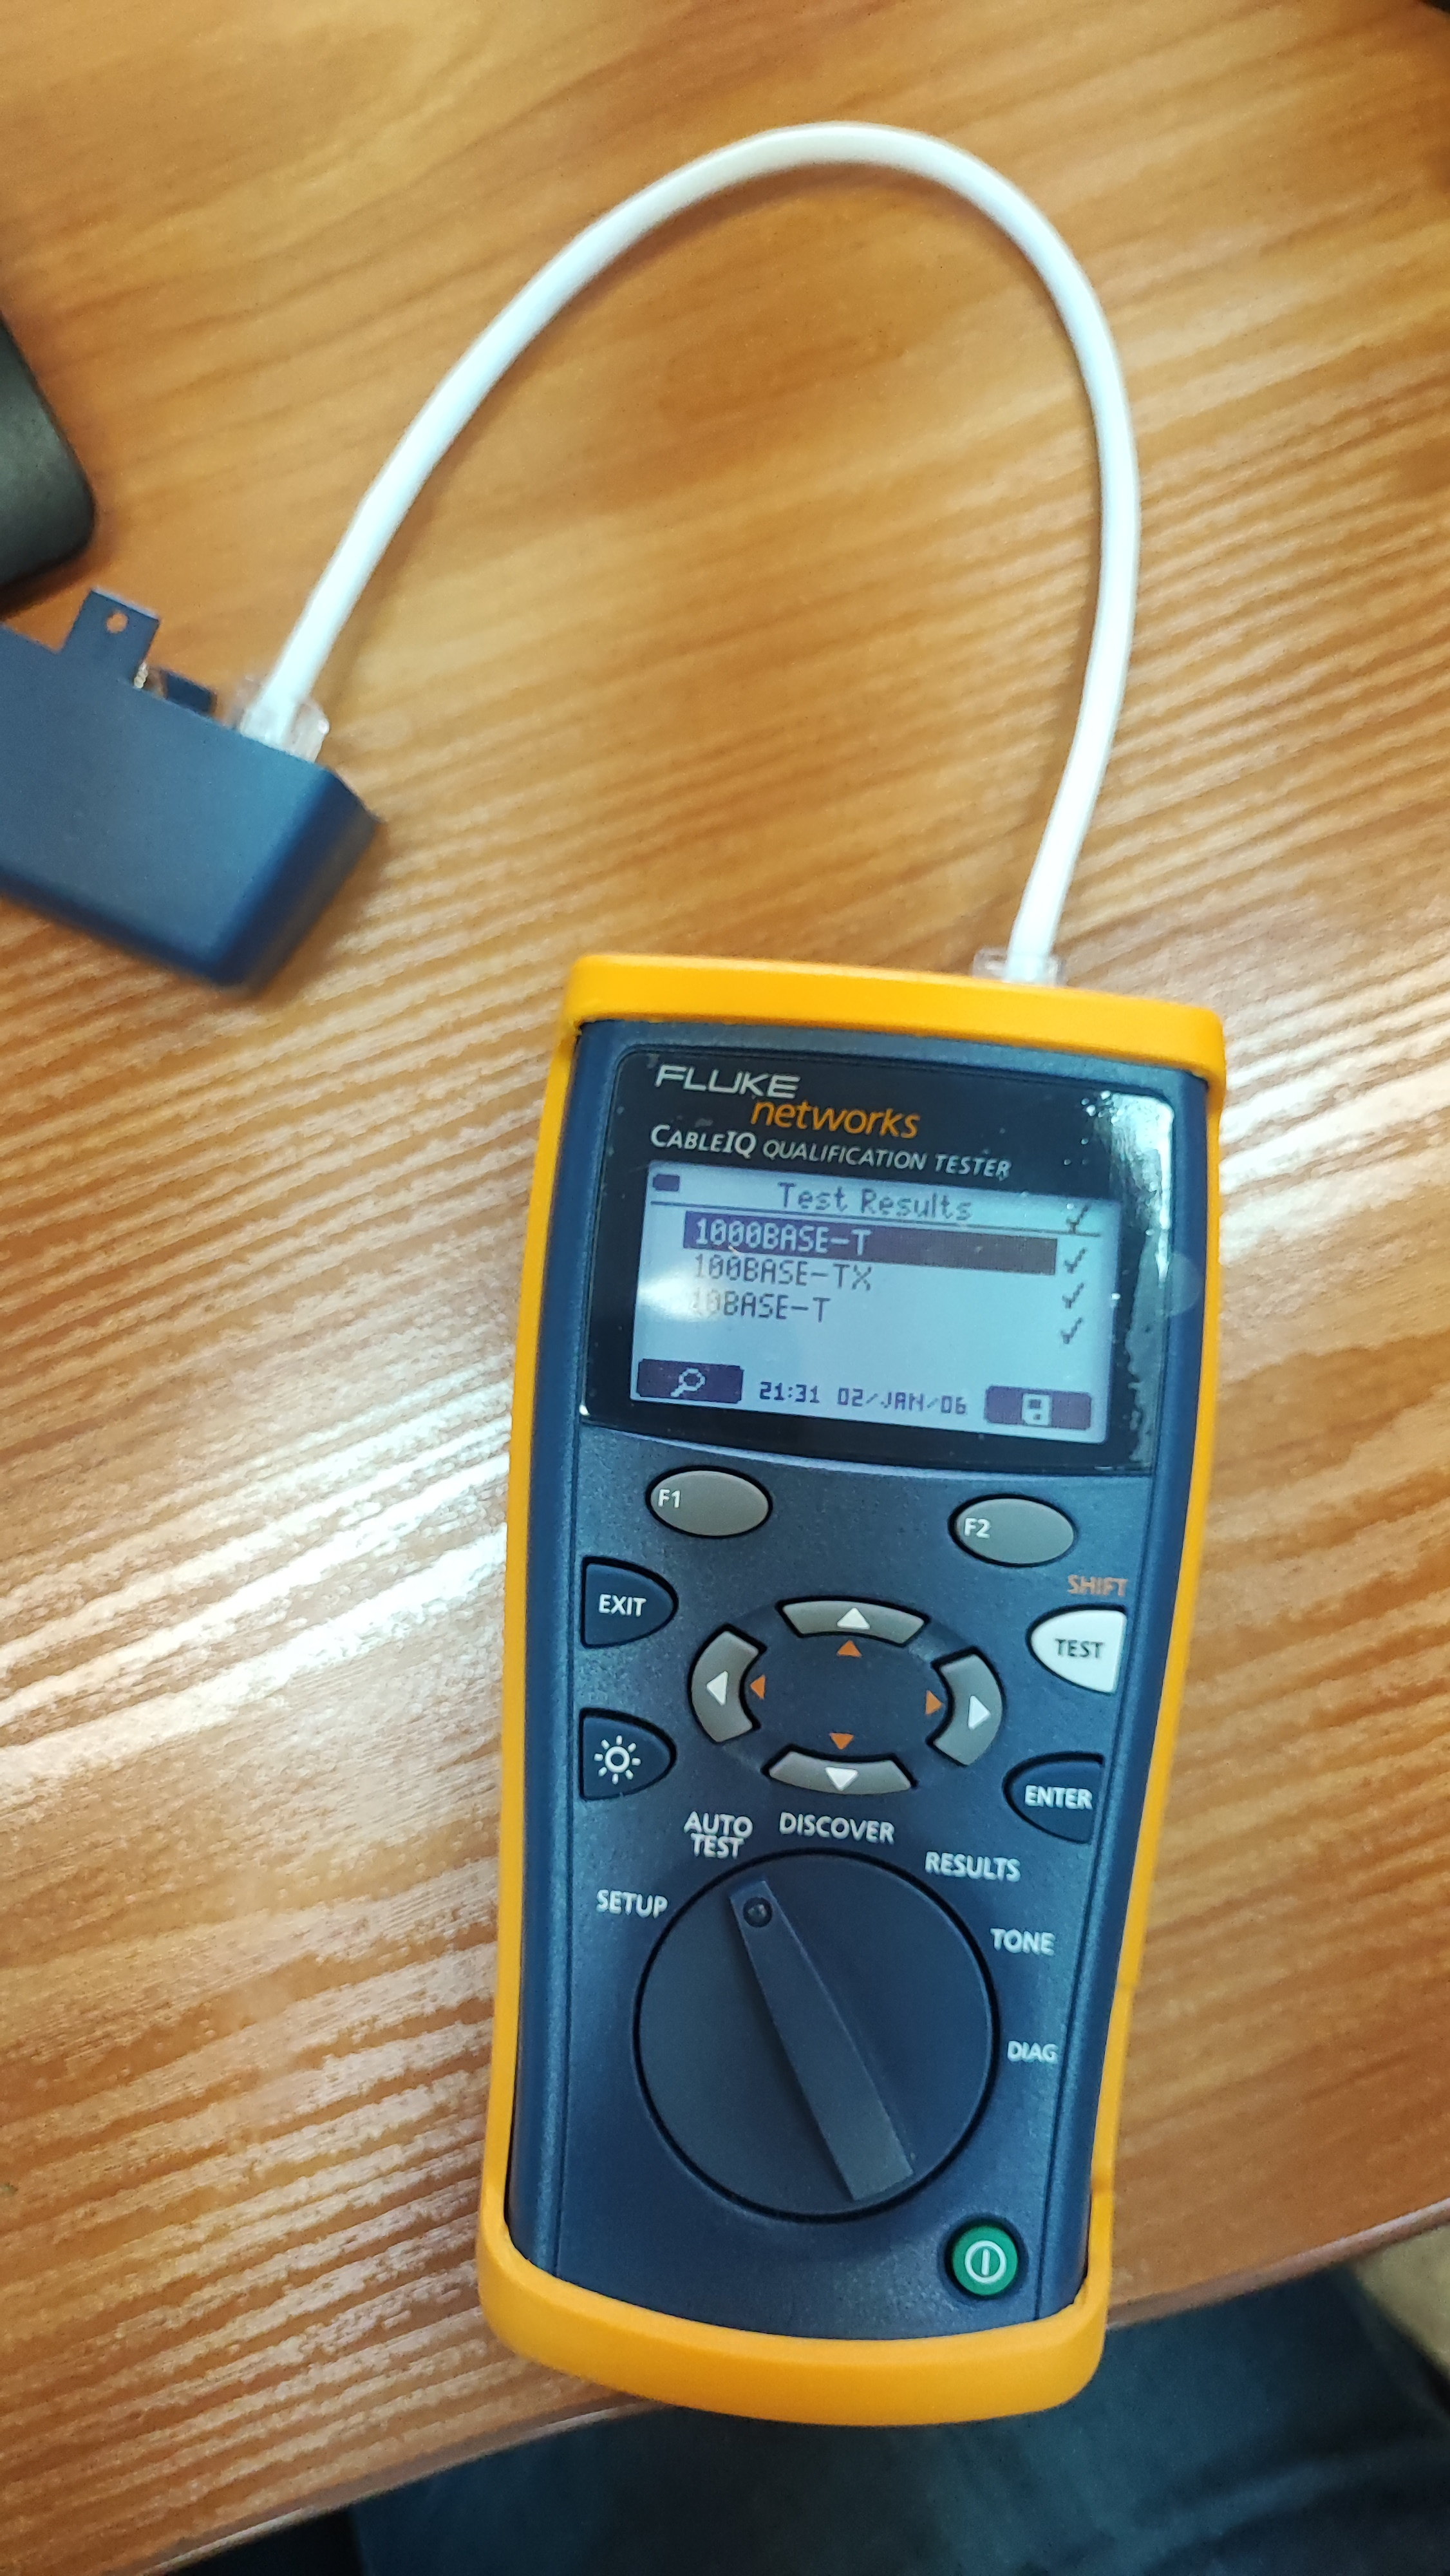
\includegraphics[height=0.31\textheight]{fluke_test_menu_1000_100_10.jpg}
\caption{Seria zdjęć 123759 i 123810: wyniki standardów oraz pomiar długości}
\end{minipage}\hfill
\begin{minipage}{0.48\textwidth}
\centering
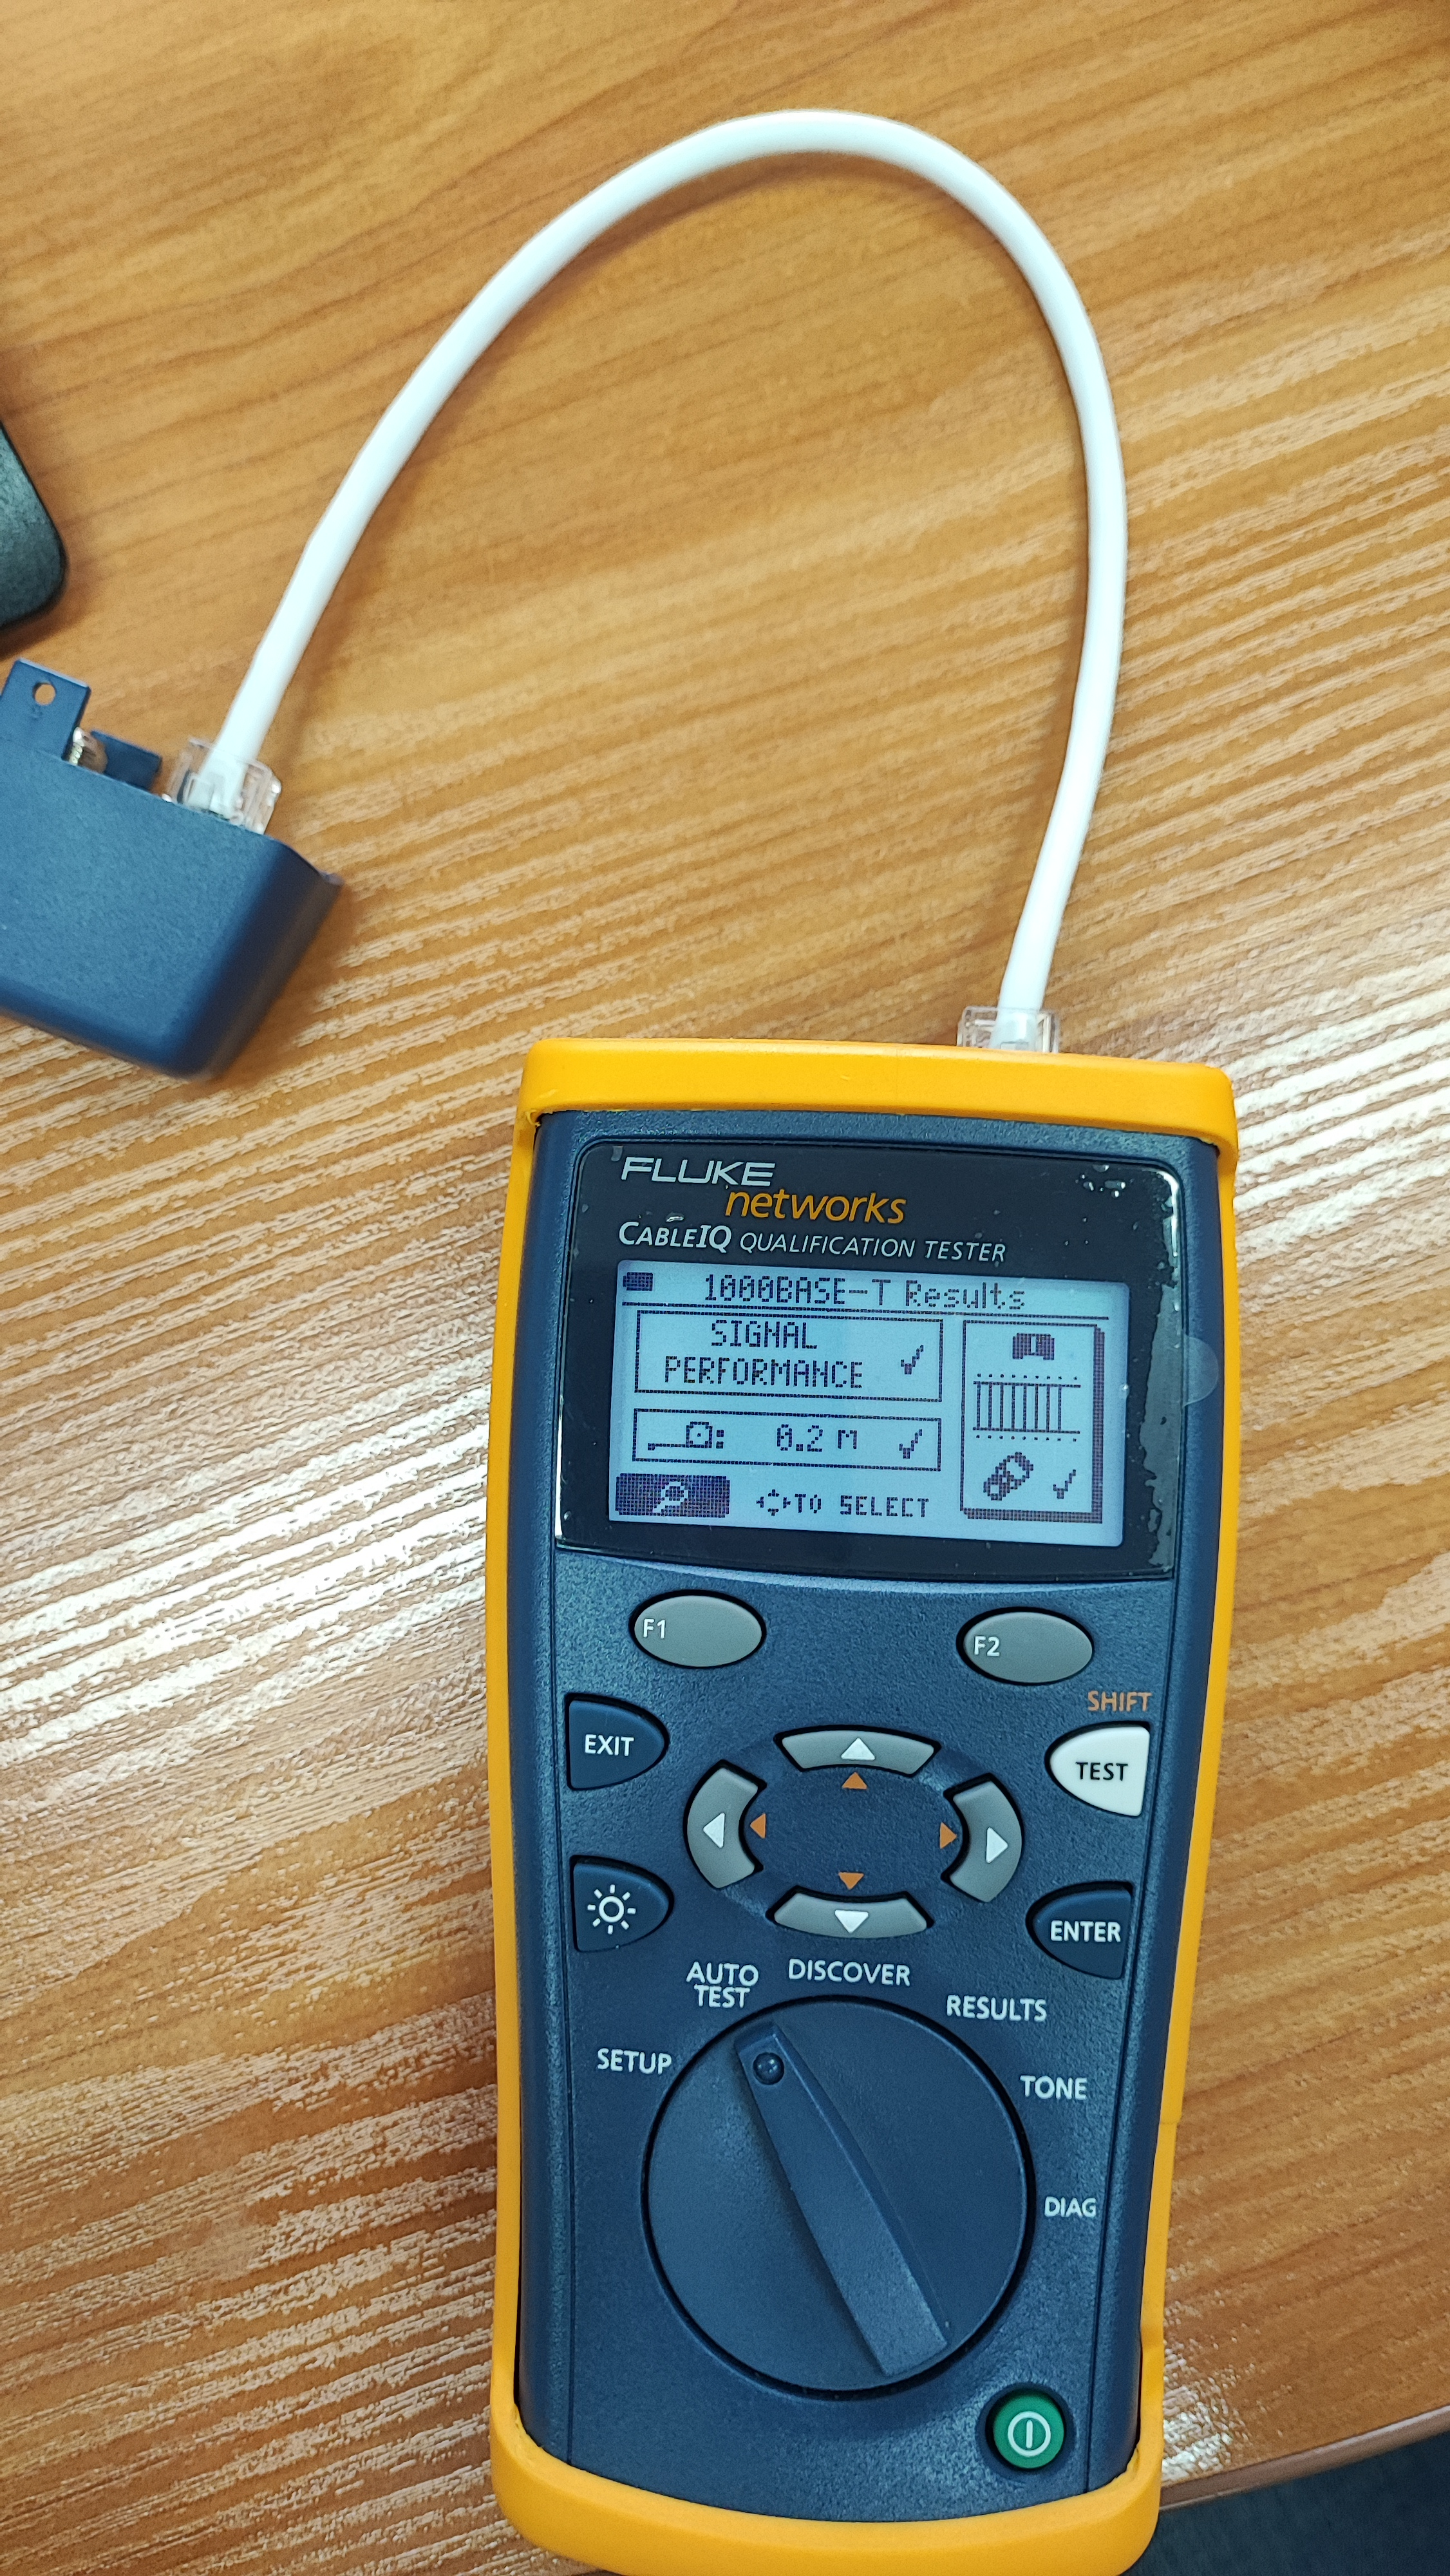
\includegraphics[height=0.31\textheight]{fluke_signal_length_0_2m.jpg}
\caption{Seria zdjęć 123759 i 123810: wyniki standardów oraz pomiar długości}
\end{minipage}
\end{figure}

\begin{figure}[H]
\centering
\begin{minipage}{0.48\textwidth}
\centering
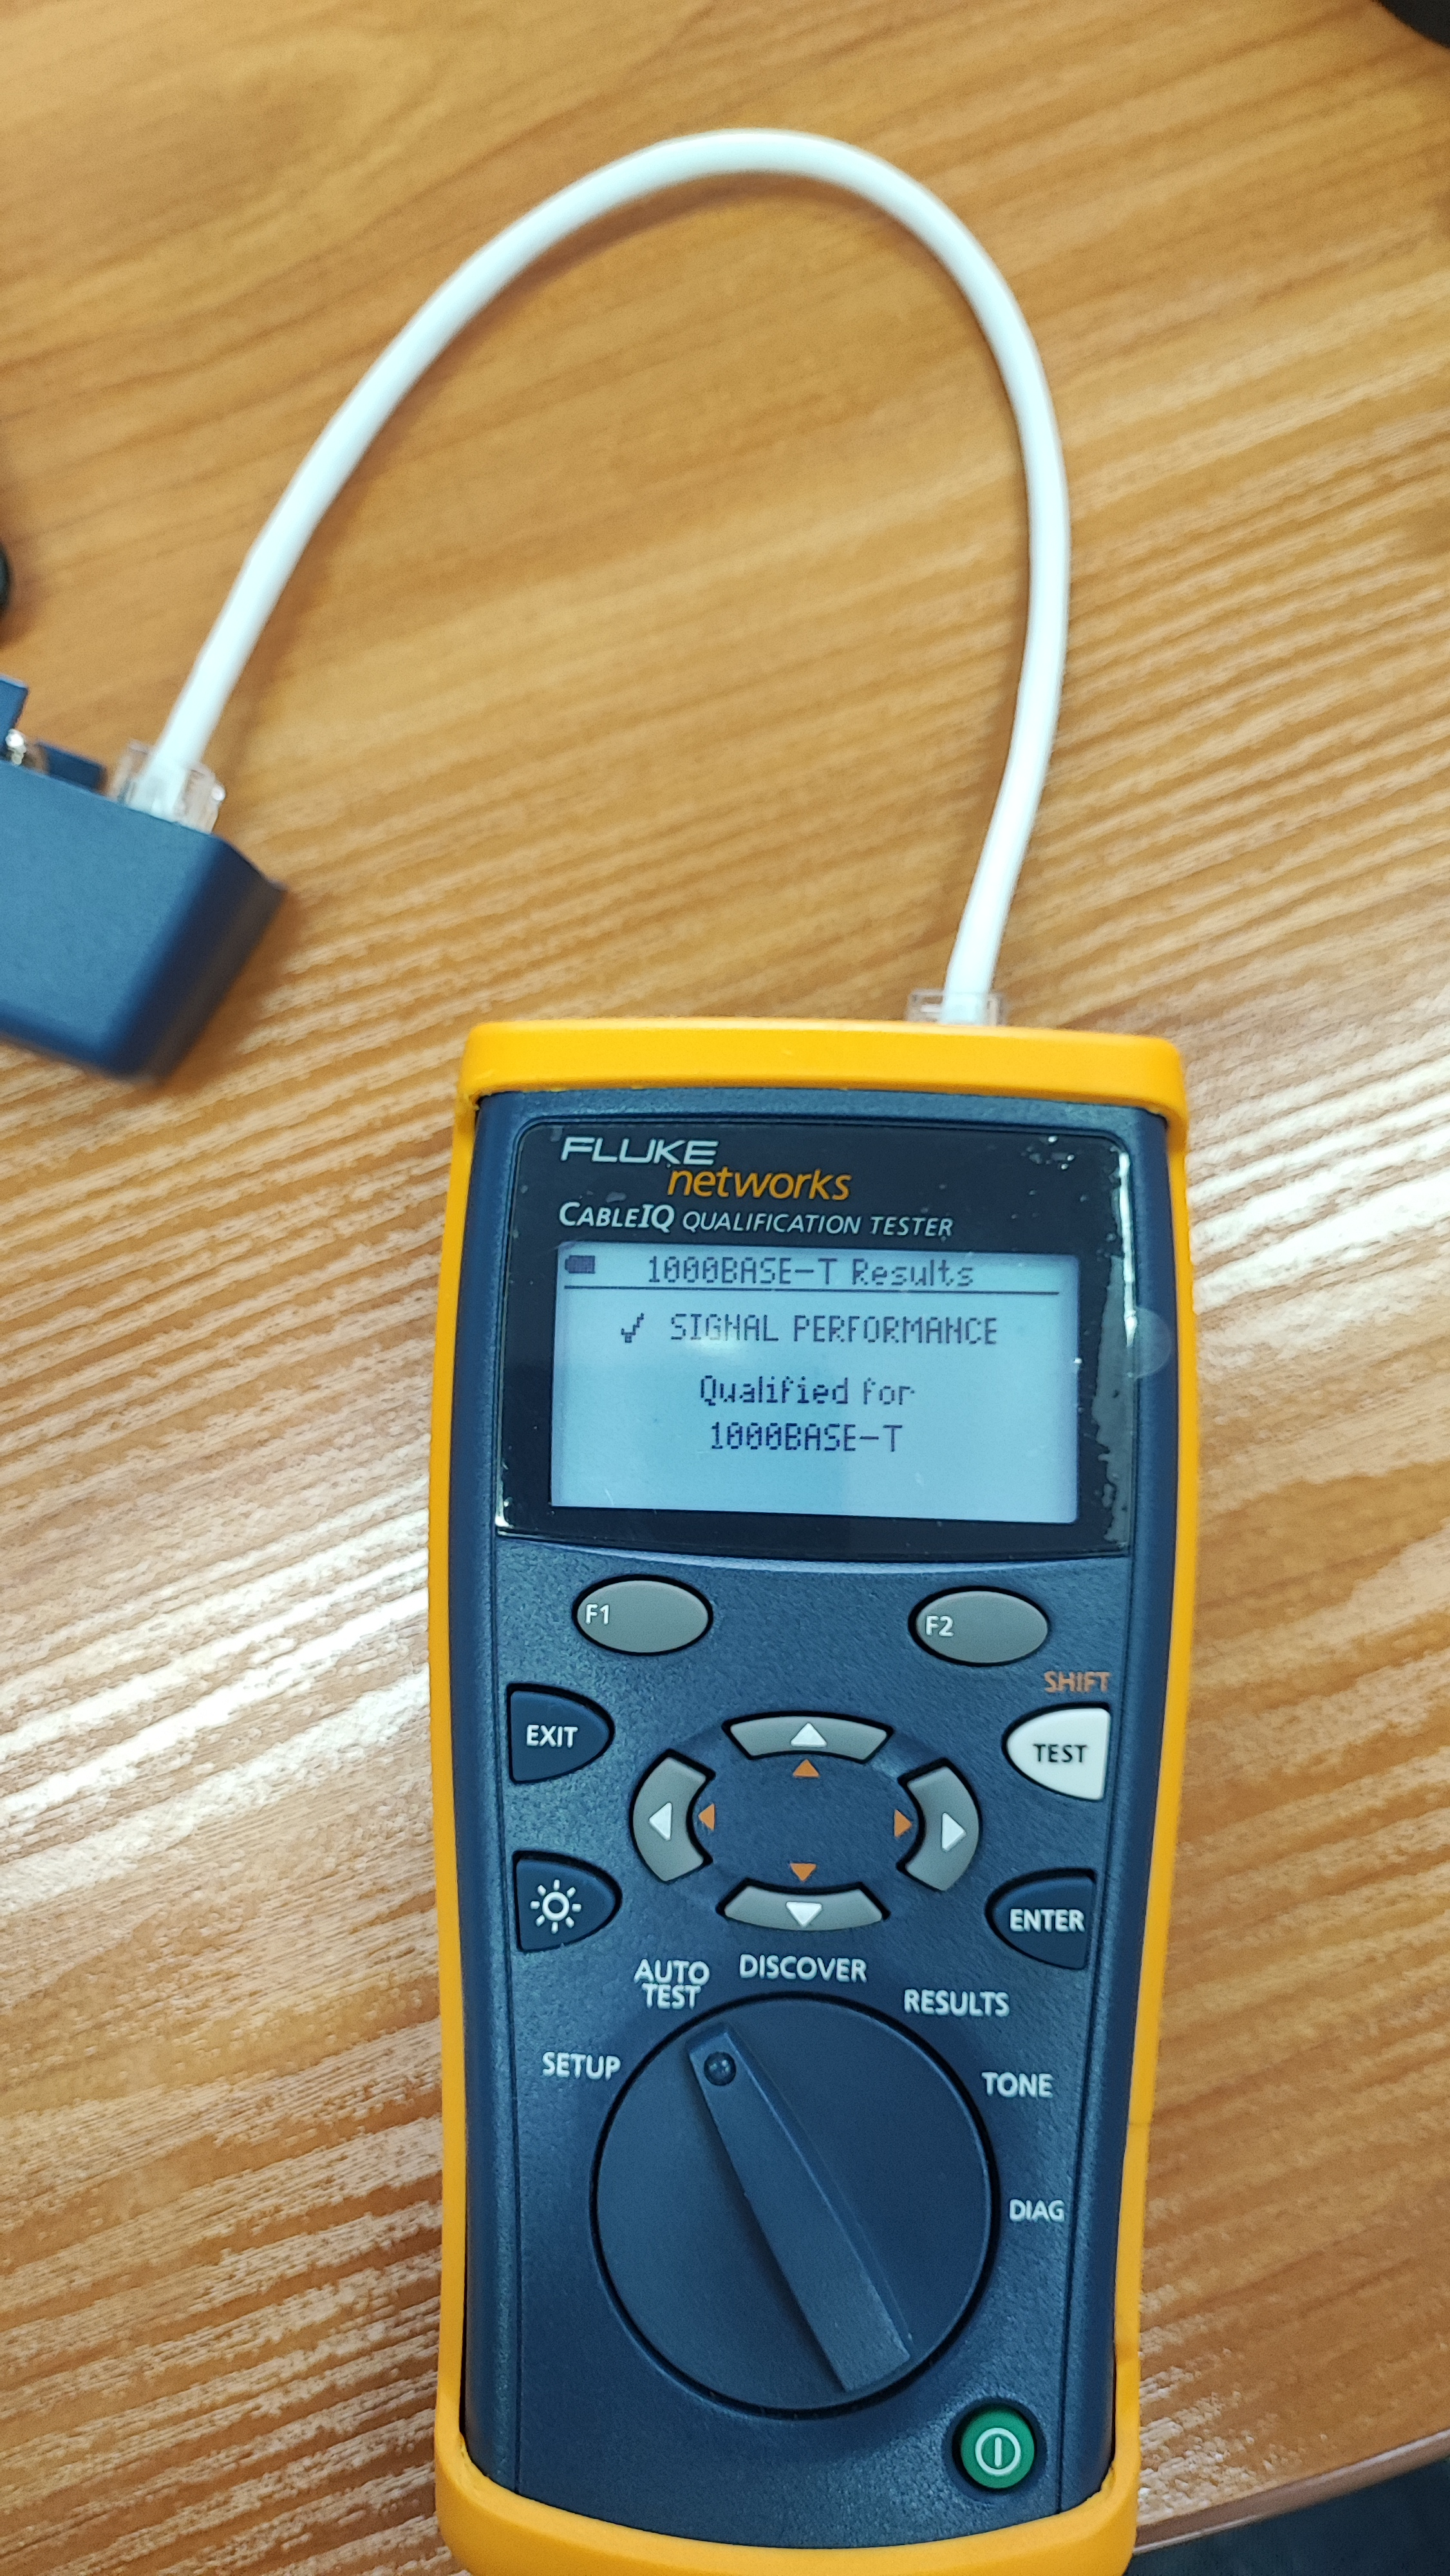
\includegraphics[height=0.31\textheight]{fluke_qualified_1000base-t.jpg}
\caption{Seria zdjęć 123825 i 123831: kwalifikacja i mapa przewodów}
\end{minipage}\hfill
\begin{minipage}{0.48\textwidth}
\centering
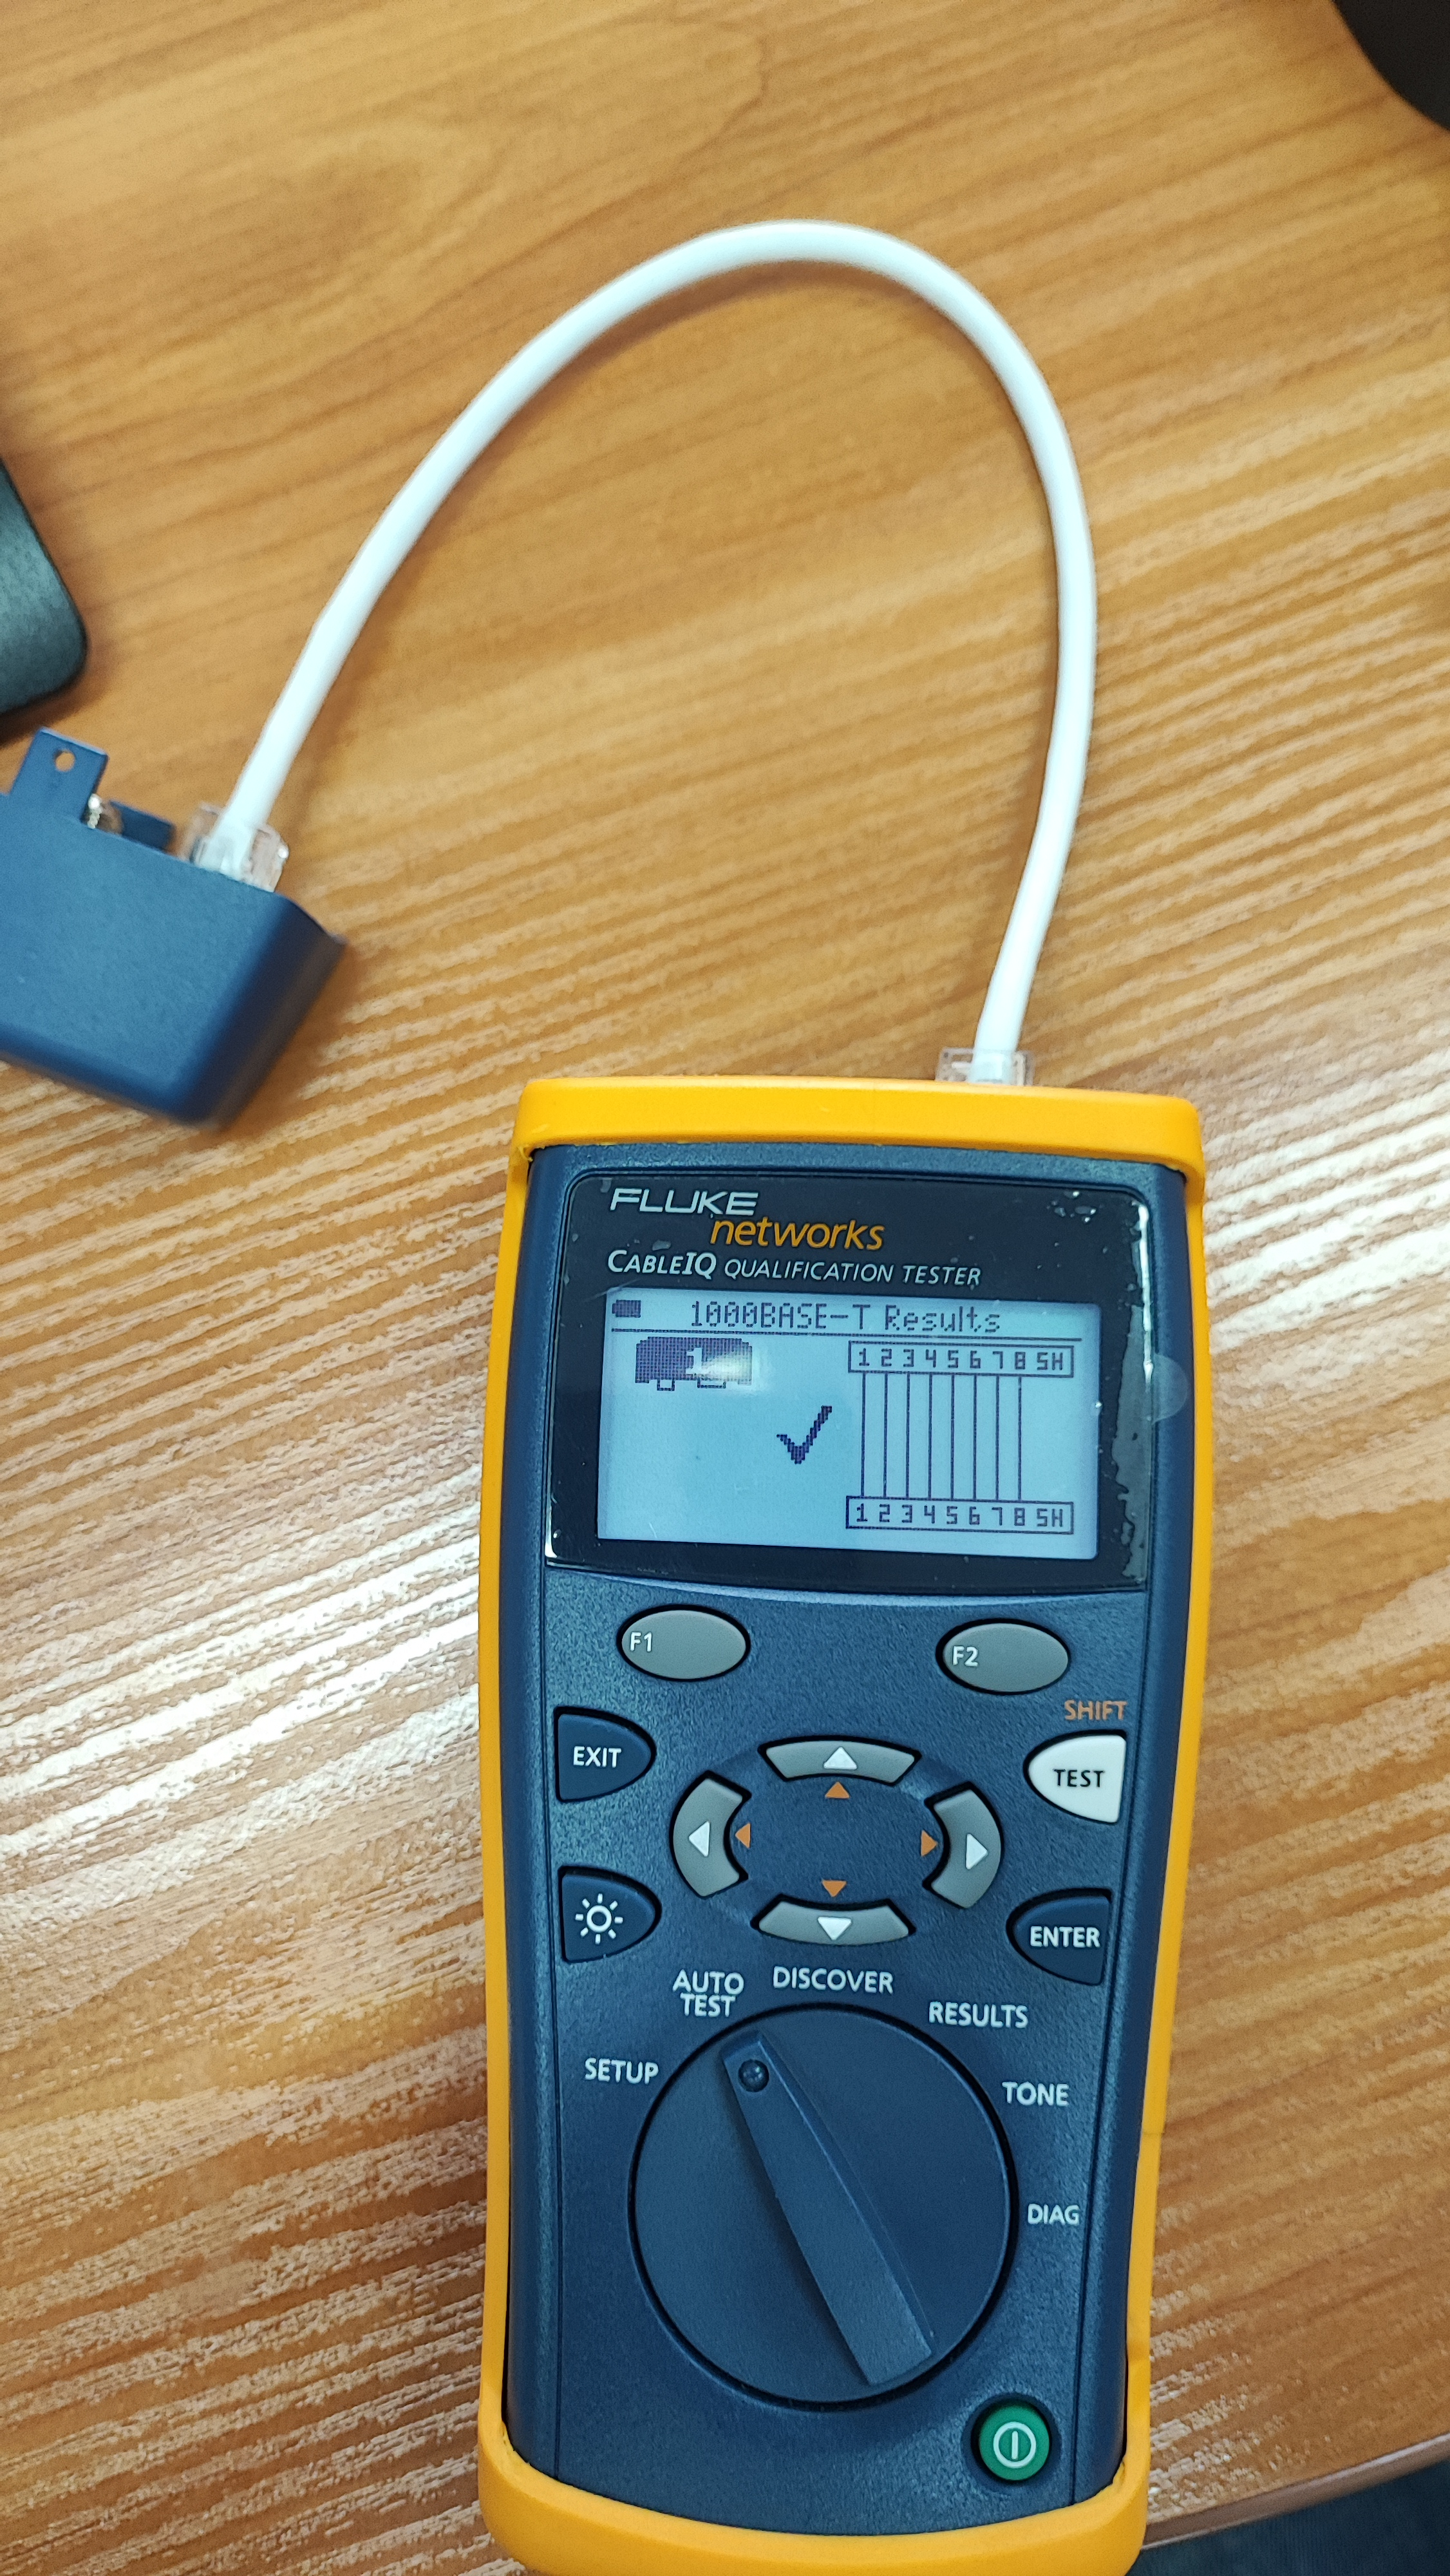
\includegraphics[height=0.31\textheight]{fluke_wiremap_correct.jpg}
\caption{Seria zdjęć 123825 i 123831: kwalifikacja i mapa przewodów}
\end{minipage}
\end{figure}

\begin{figure}[H]
\centering
\begin{minipage}{0.48\textwidth}
\centering
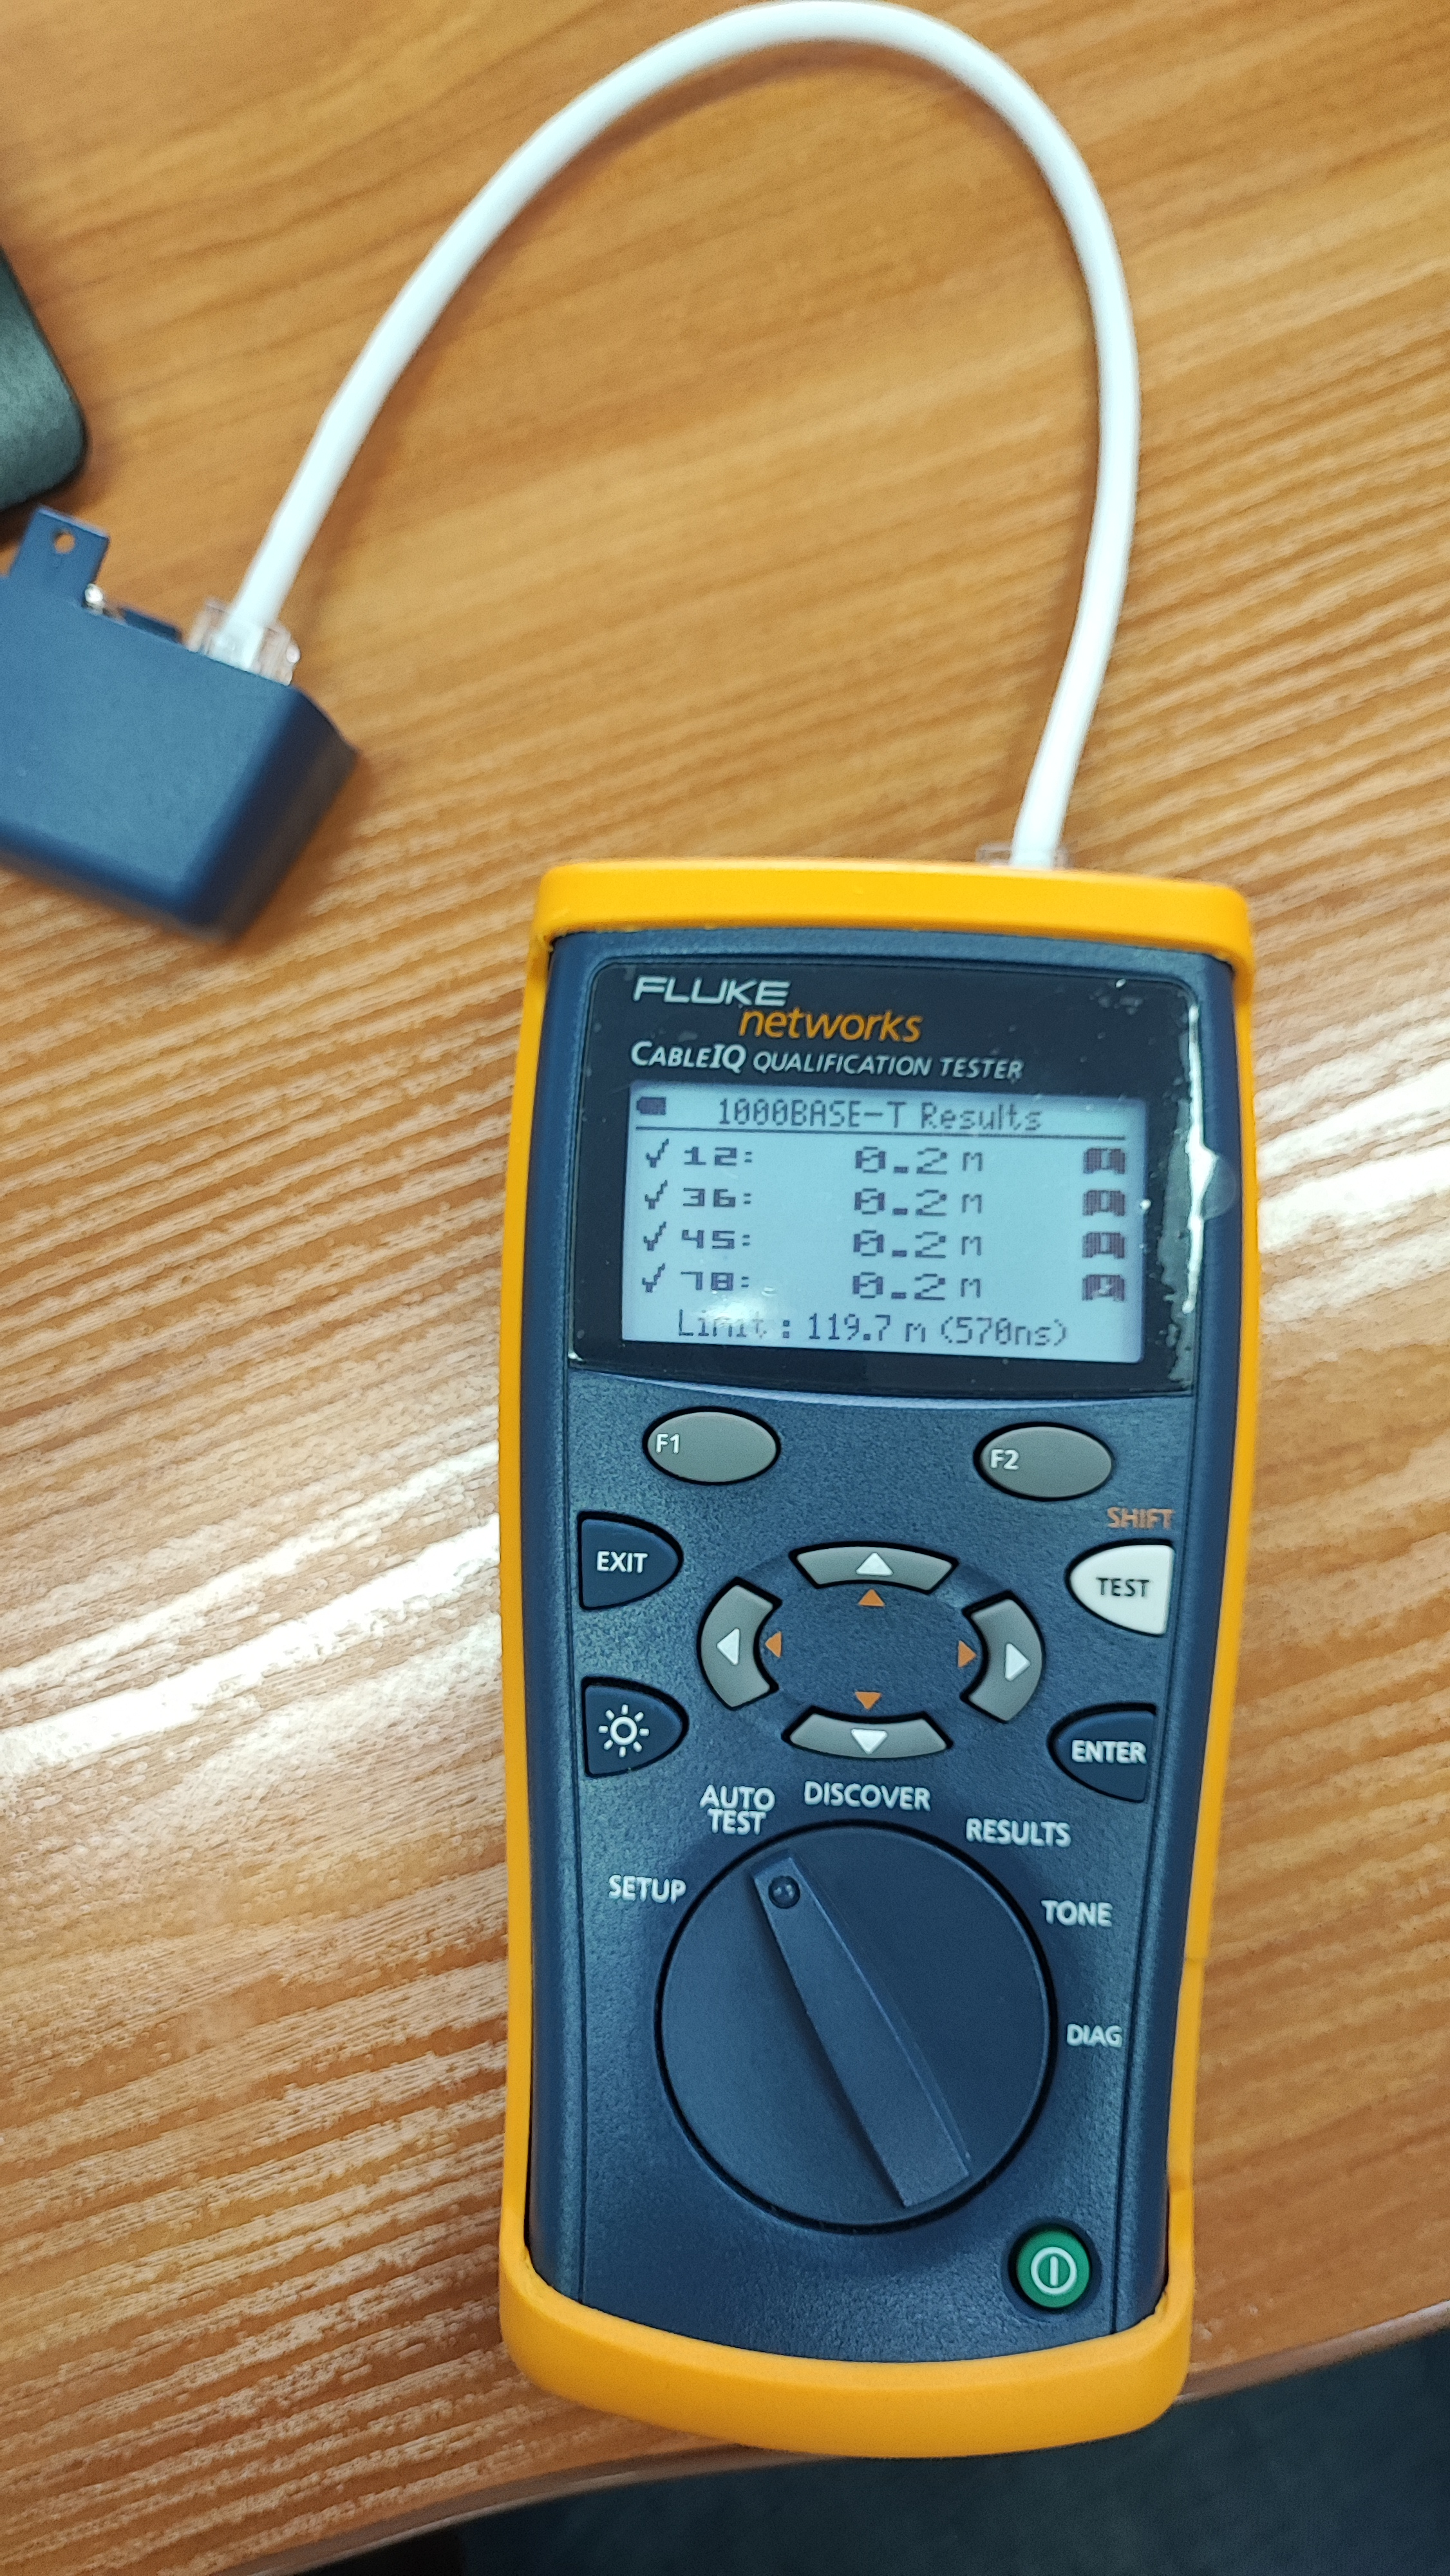
\includegraphics[height=0.31\textheight]{fluke_pairs_lengths_0_2m.jpg}
\caption{Seria zdjęć 123842 i 124127: długości par i kolejny test}
\end{minipage}\hfill
\begin{minipage}{0.48\textwidth}
\centering
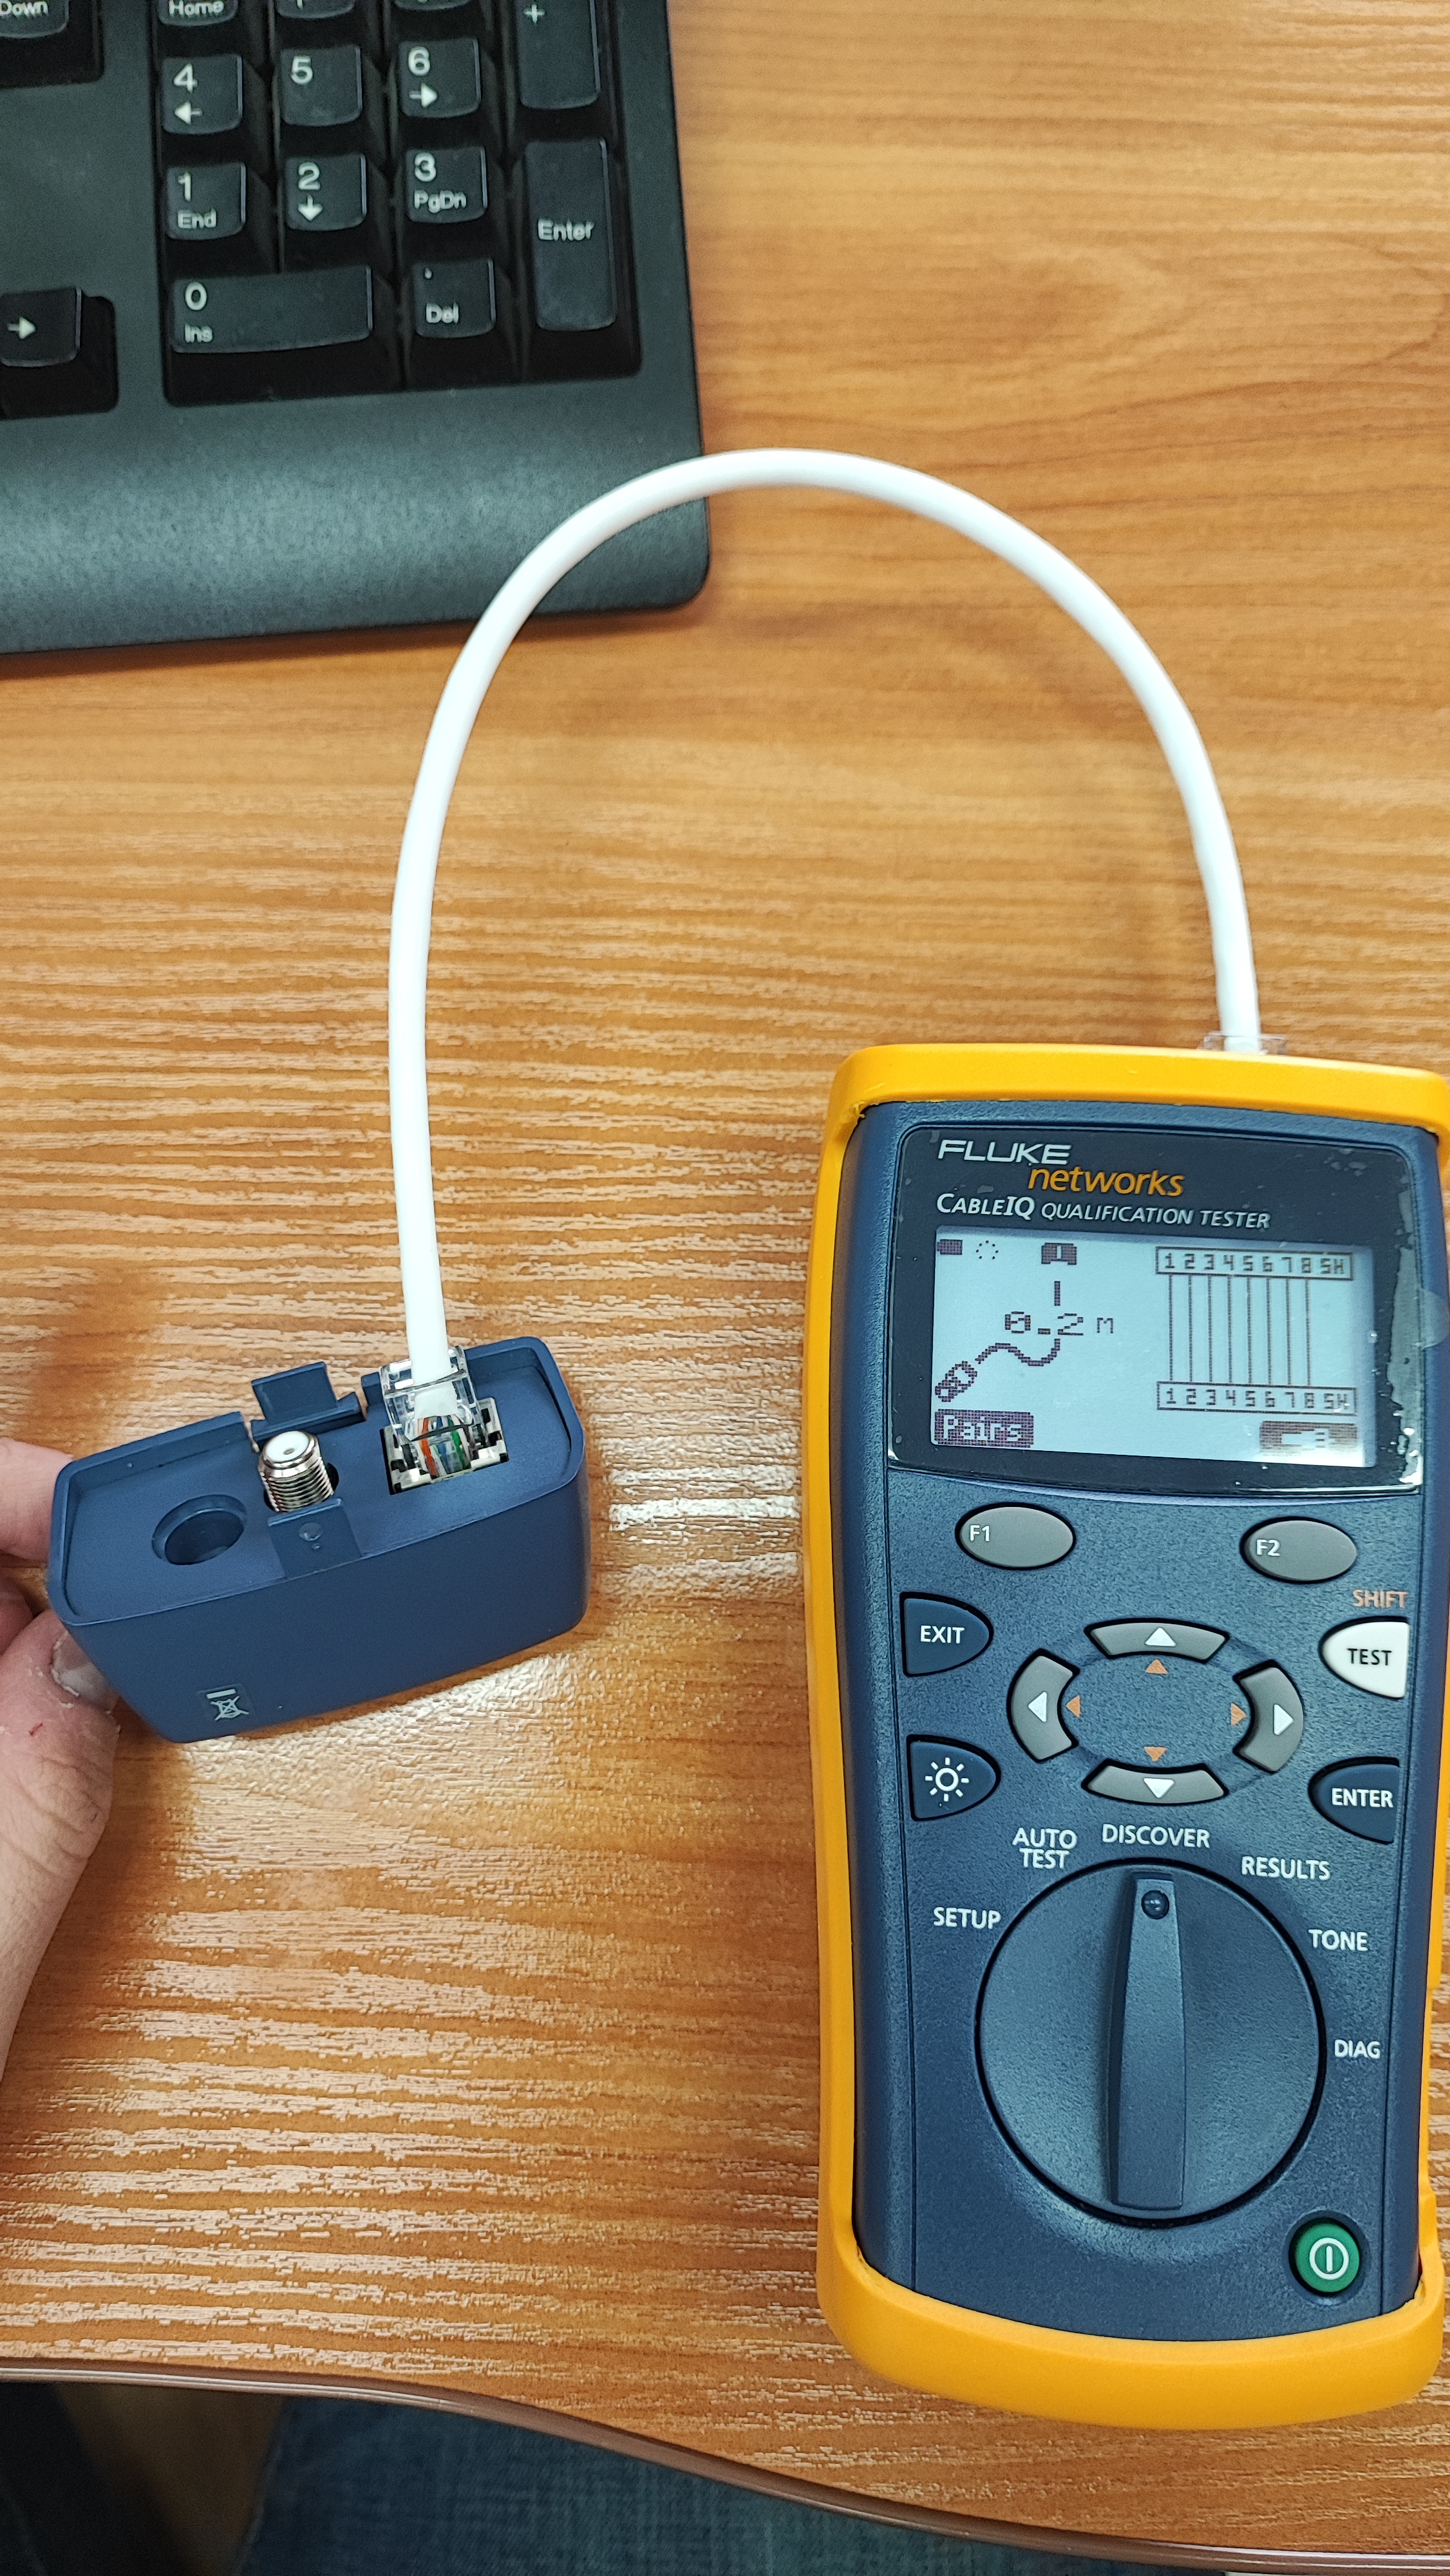
\includegraphics[height=0.31\textheight]{fluke_pairs_wiremap_0_1m.jpg}
\caption{Seria zdjęć 123842 i 124127: długości par i kolejny test}
\end{minipage}
\end{figure}

\begin{figure}[H]
\centering
\begin{minipage}{0.48\textwidth}
\centering
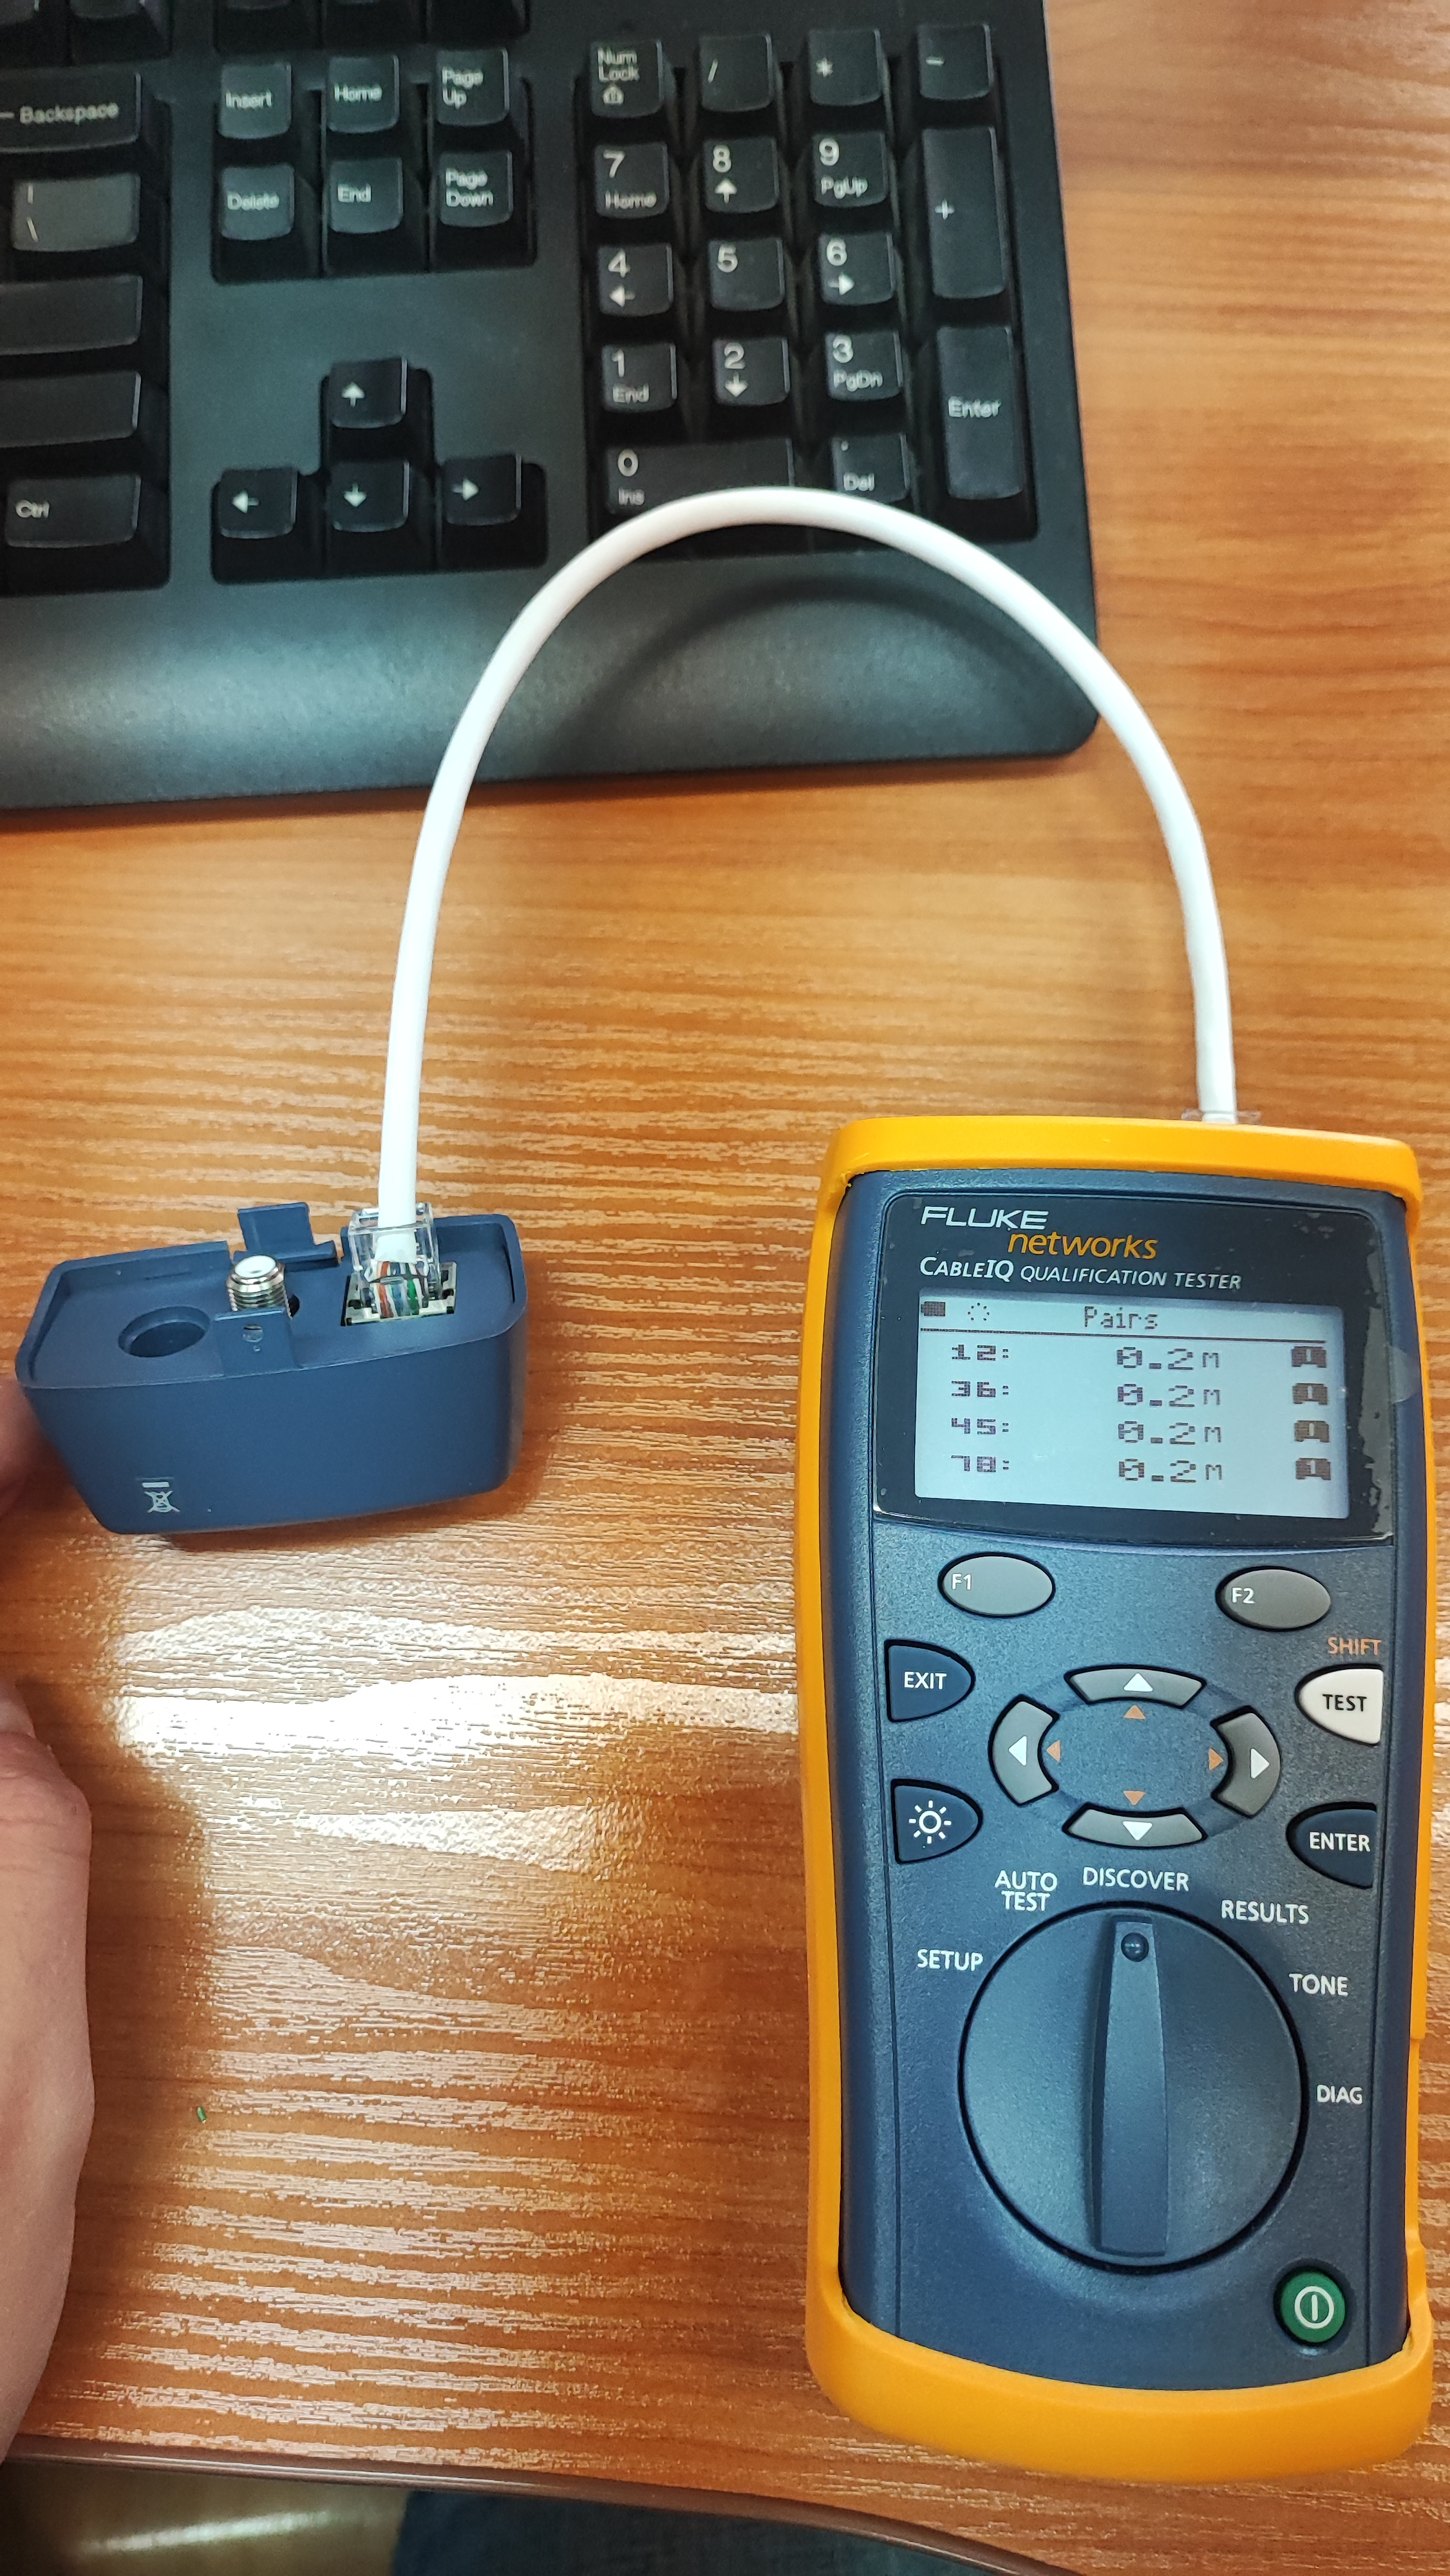
\includegraphics[height=0.31\textheight]{fluke_pair_length_second_test.jpg}
\caption{Seria zdjęć 124242 i 124400: kolejne pomiary patchcorda}
\end{minipage}\hfill
\begin{minipage}{0.48\textwidth}
\centering
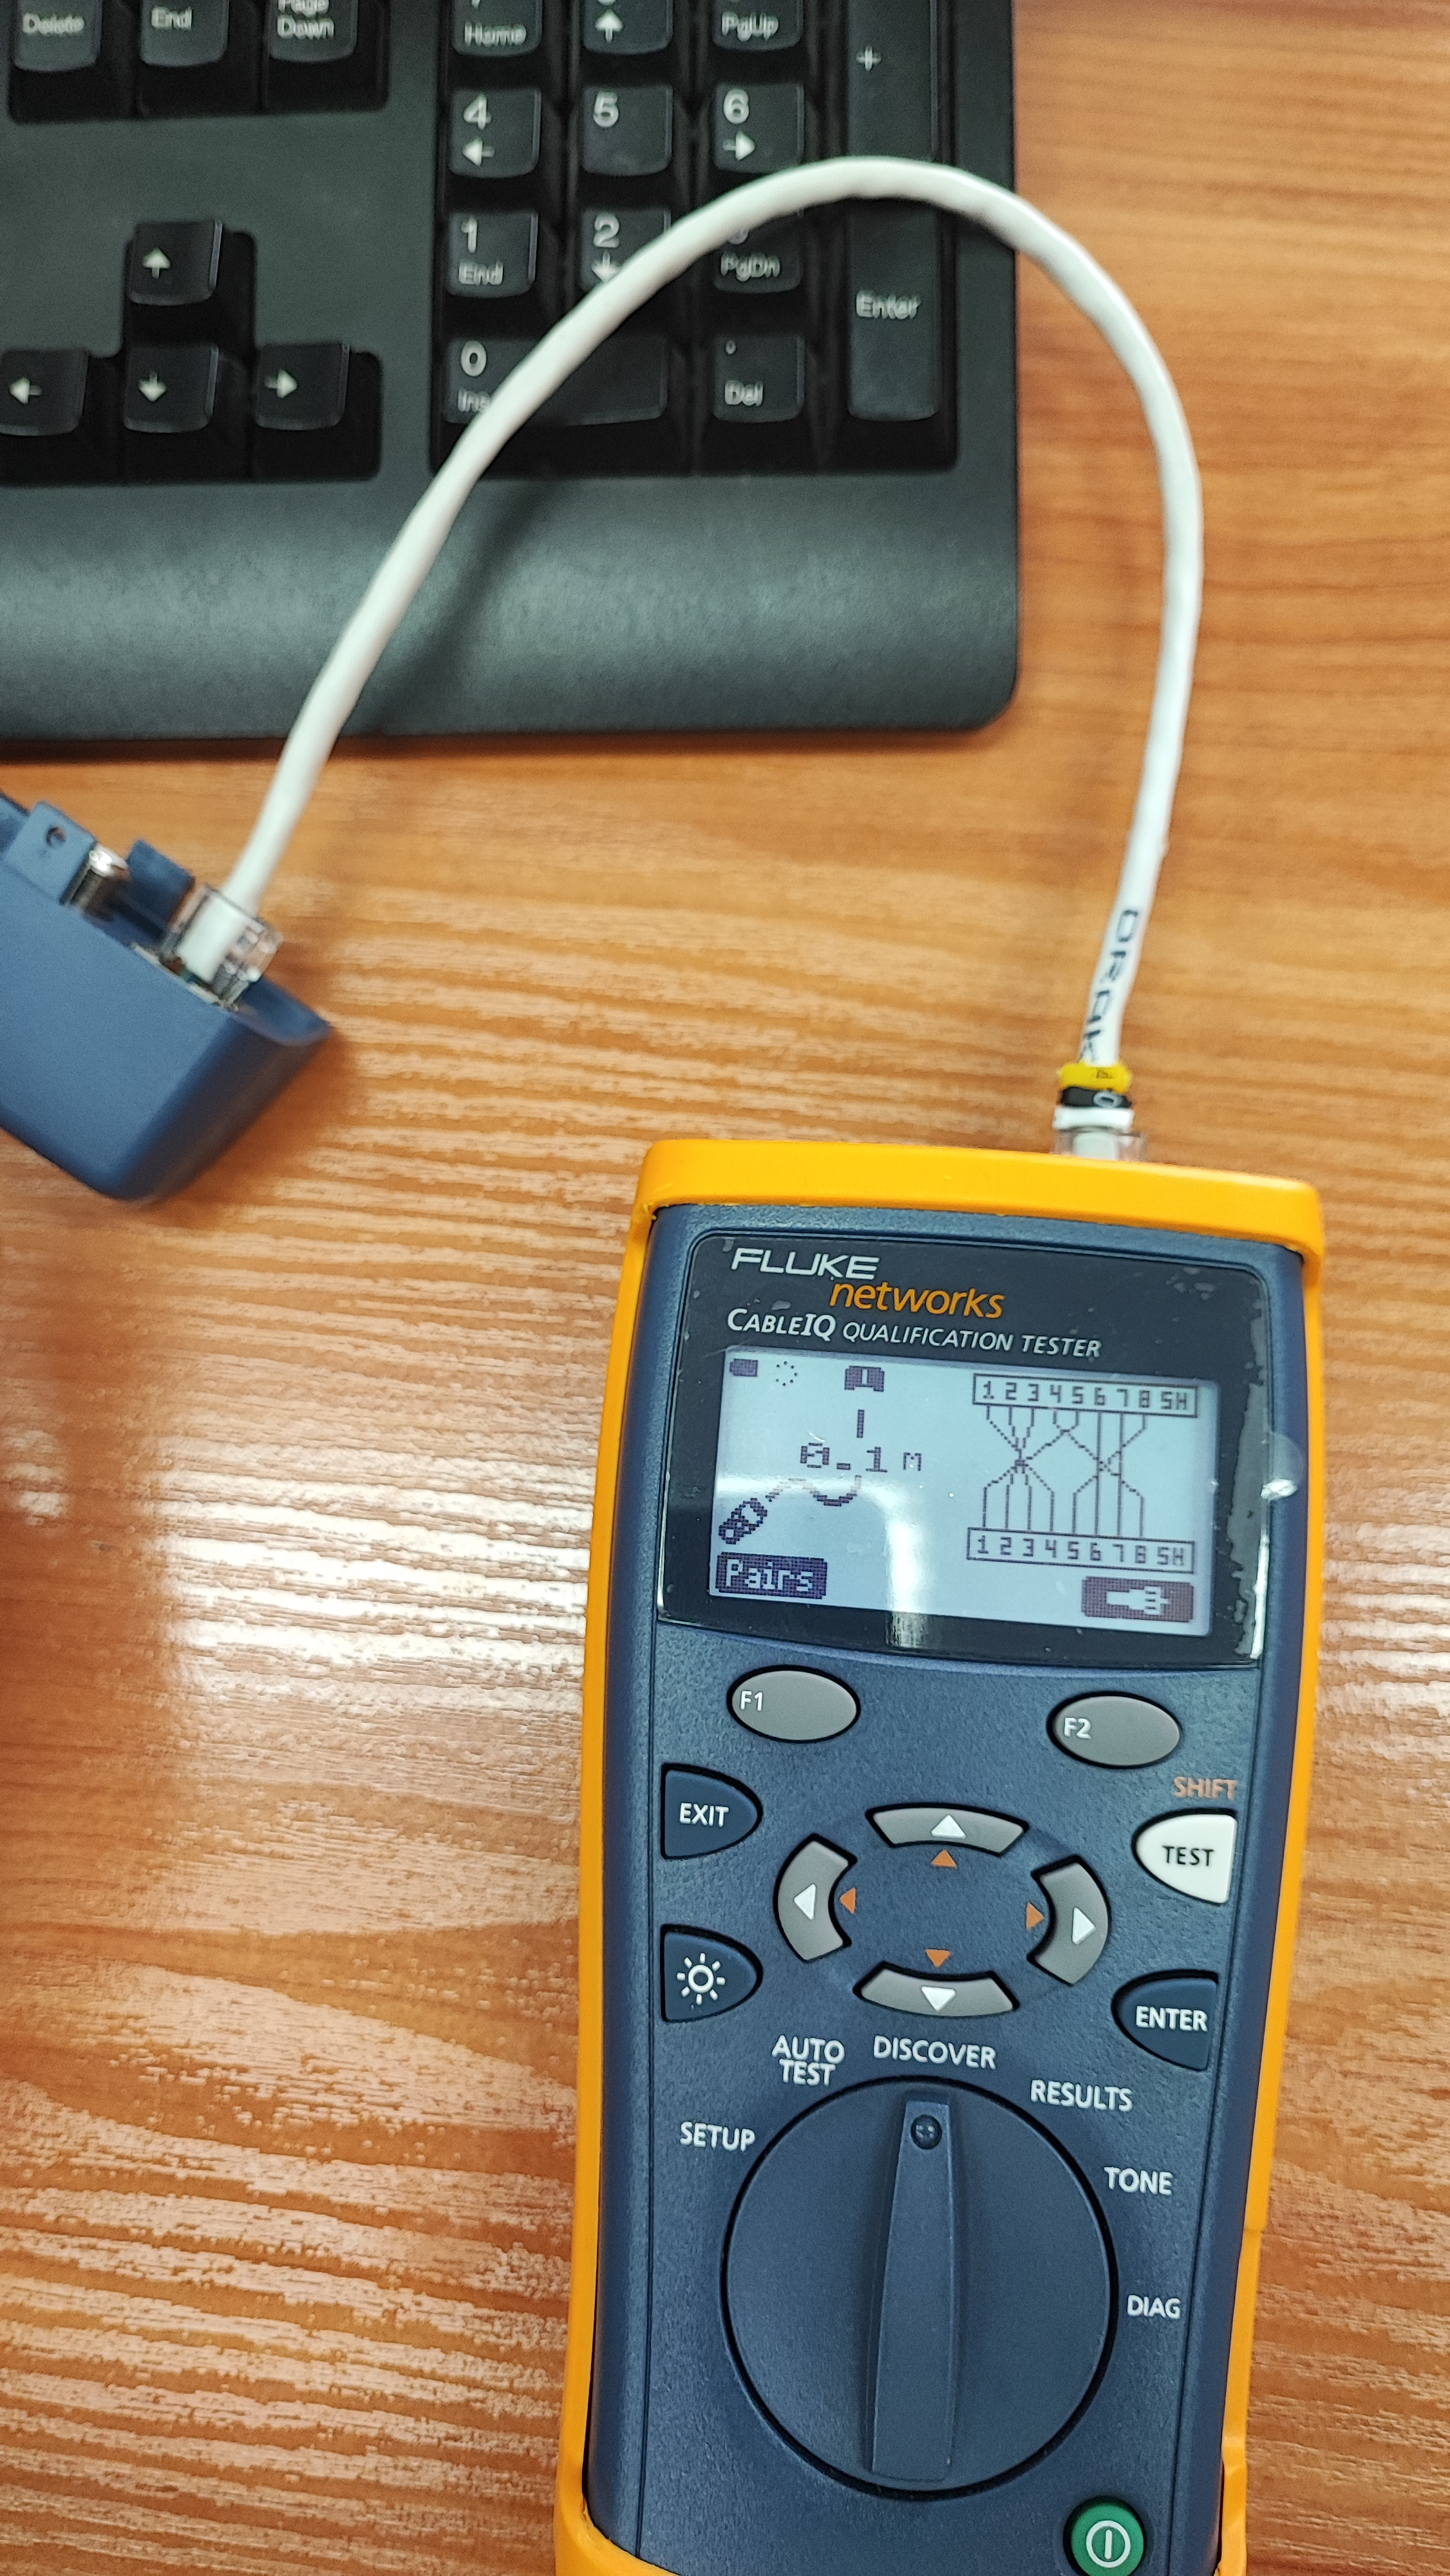
\includegraphics[height=0.31\textheight]{fluke_wiremap_length_0_1m.jpg}
\caption{Seria zdjęć 124242 i 124400: kolejne pomiary patchcorda}
\end{minipage}
\end{figure}

\begin{figure}[H]
\centering
\begin{minipage}{0.48\textwidth}
\centering
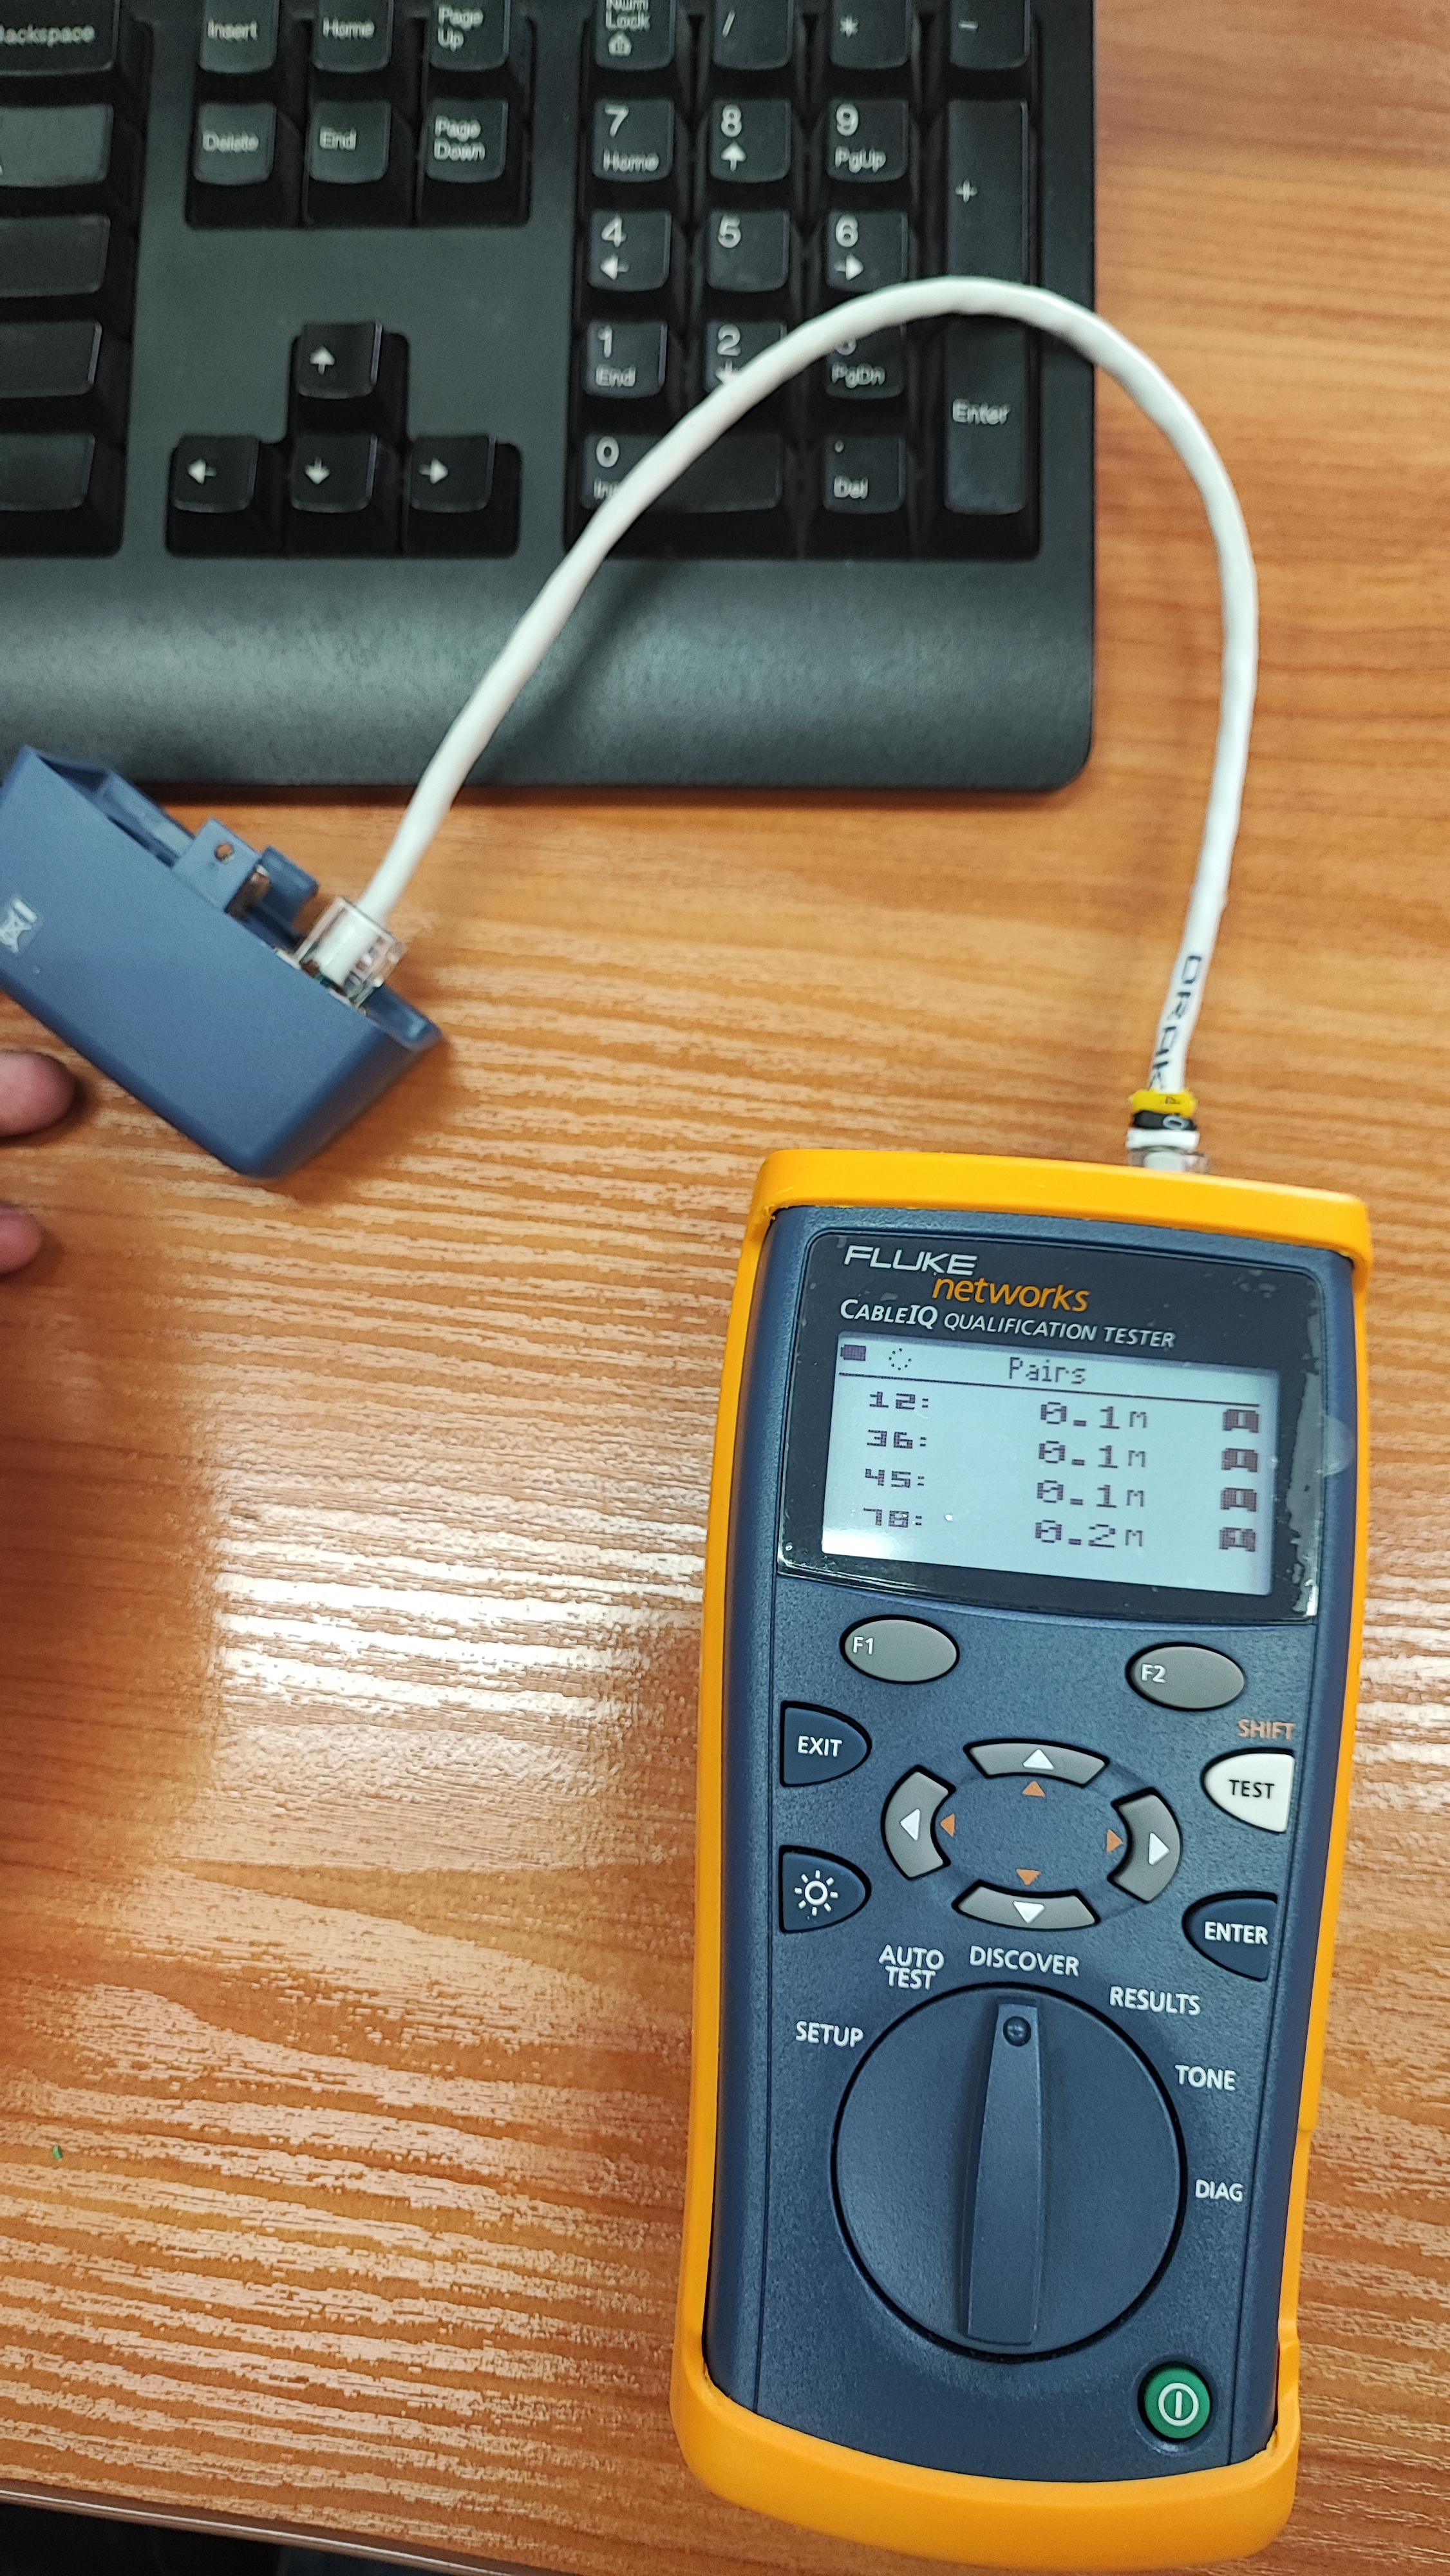
\includegraphics[height=0.31\textheight]{fluke_pairs_length_0_1_0_2m.jpg}
\caption{Seria zdjęć 124407 i 124421: długości par i wynik standardów}
\end{minipage}\hfill
\begin{minipage}{0.48\textwidth}
\centering
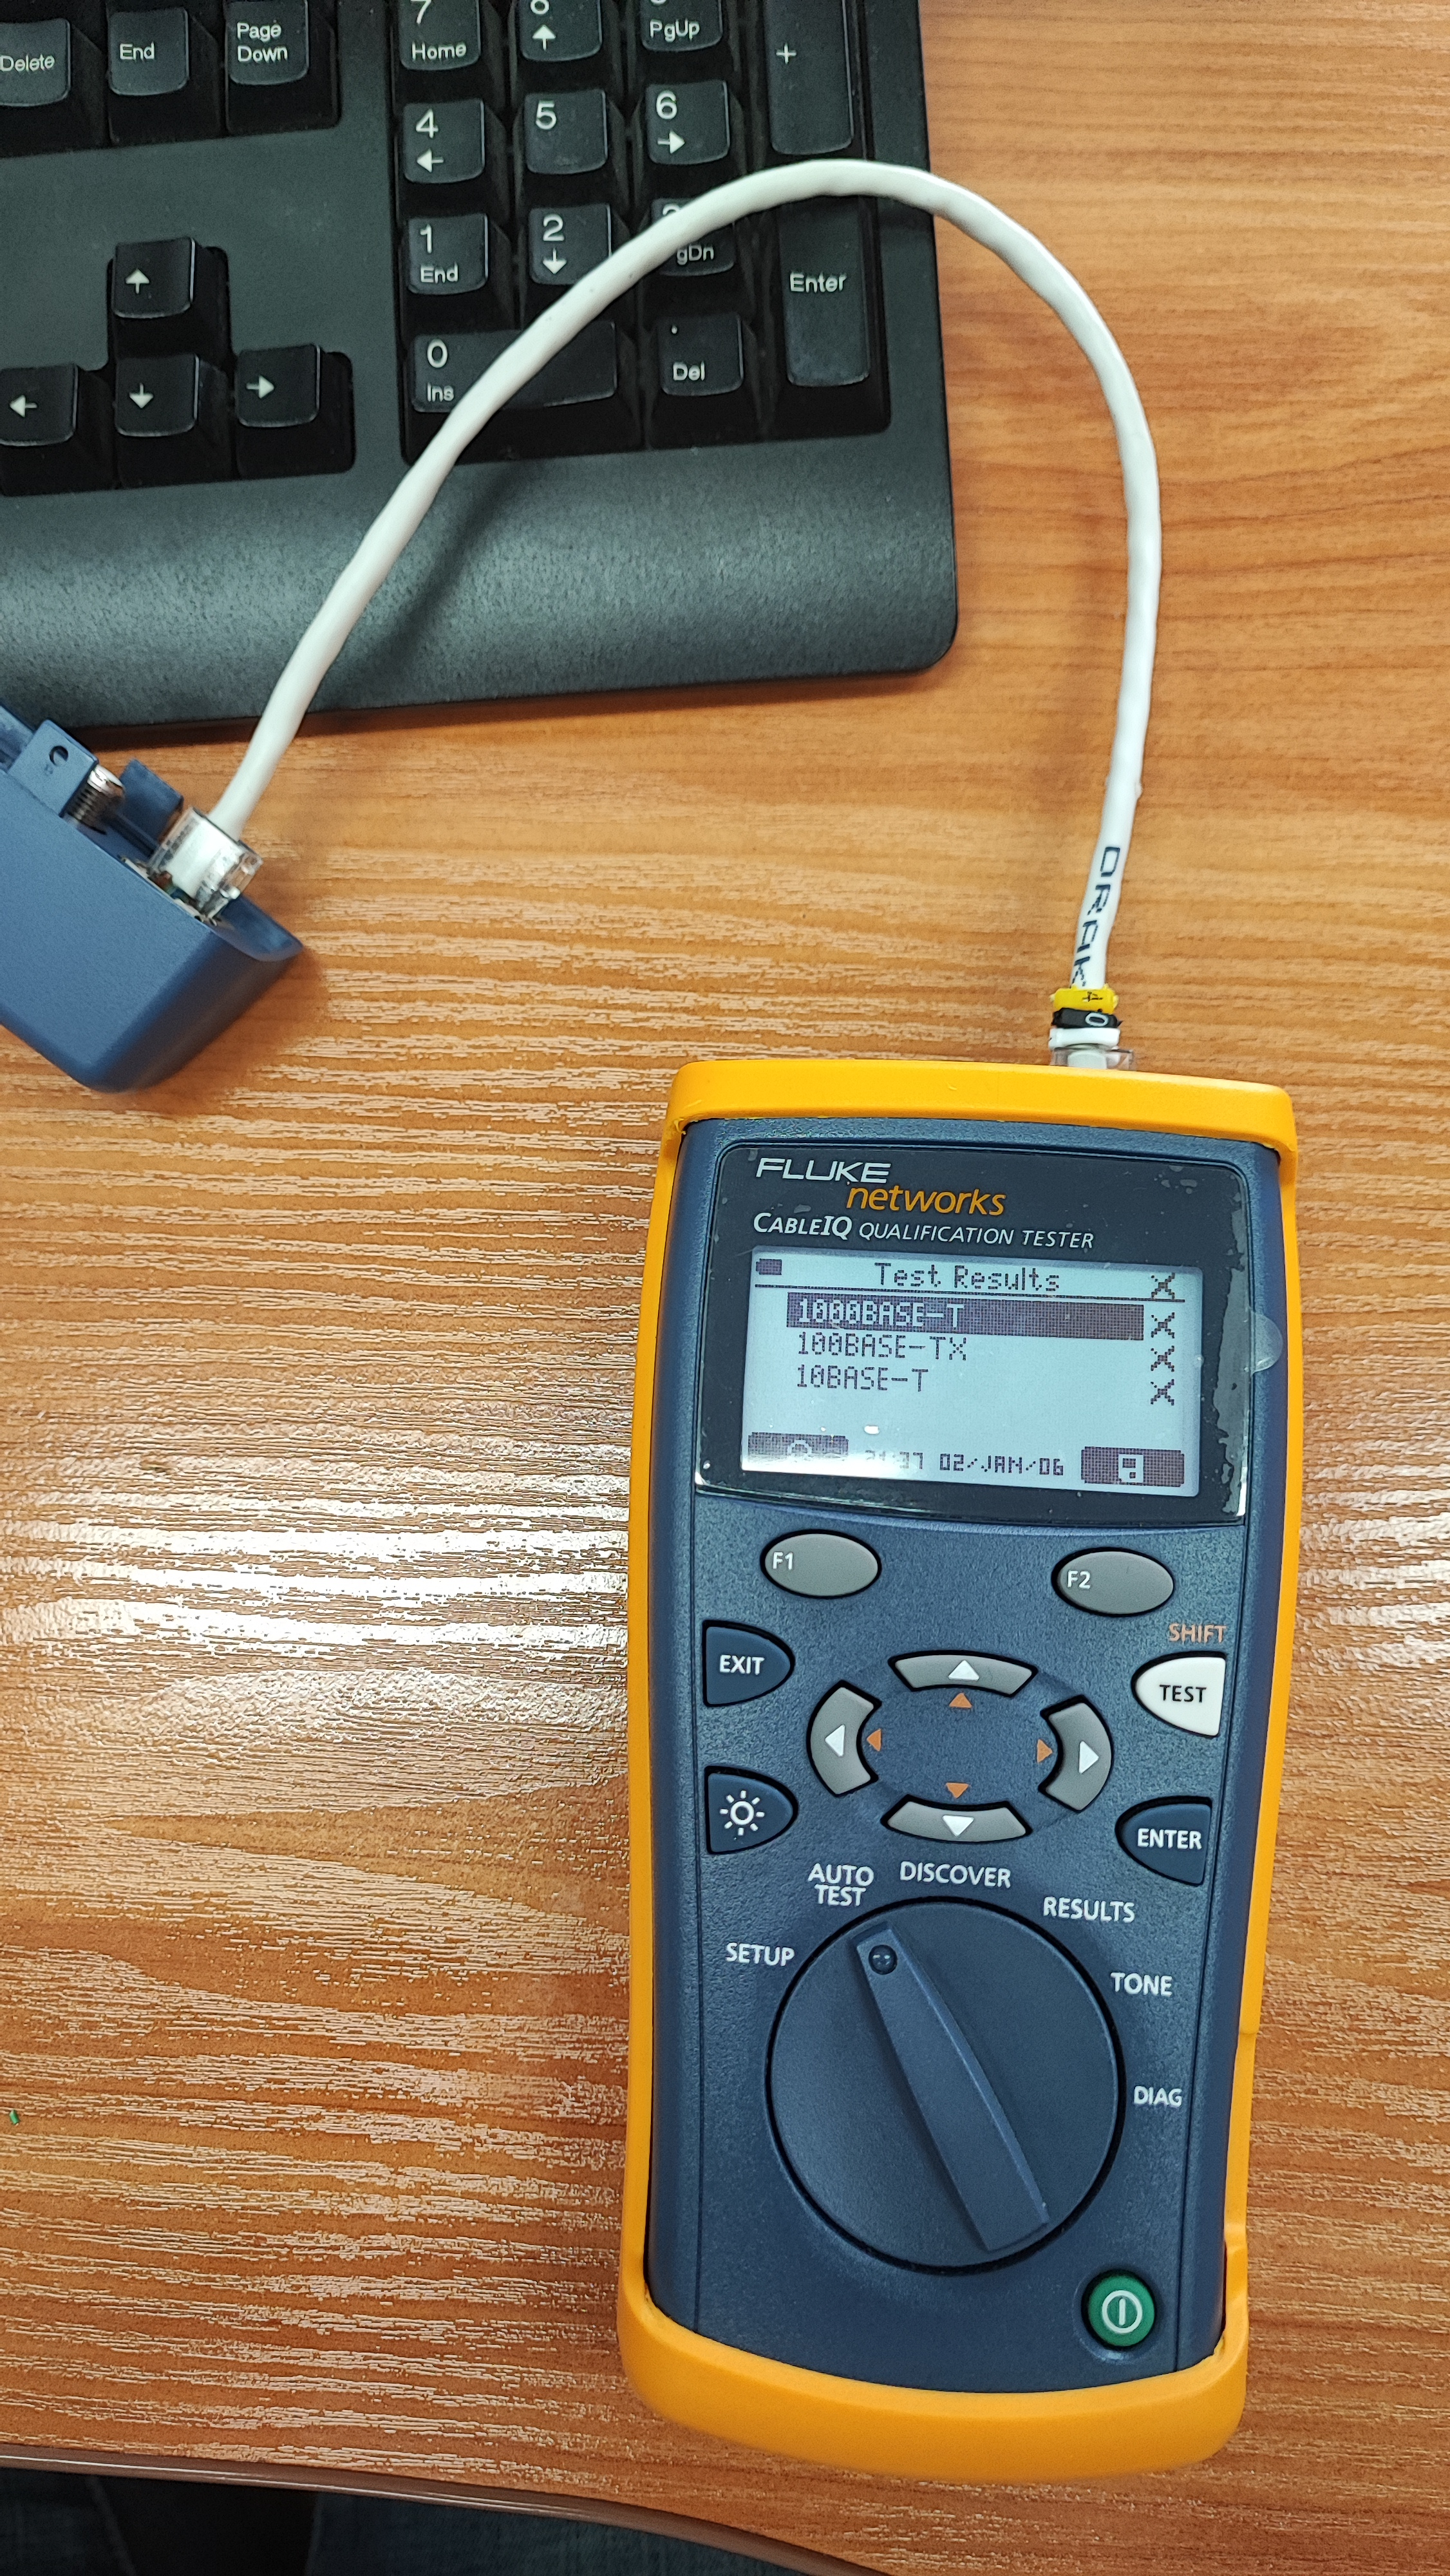
\includegraphics[height=0.31\textheight]{fluke_test_results_1000_100_10.jpg}
\caption{Seria zdjęć 124407 i 124421: długości par i wynik standardów}
\end{minipage}
\end{figure}

\begin{figure}[H]
\centering
\begin{minipage}{0.48\textwidth}
\centering
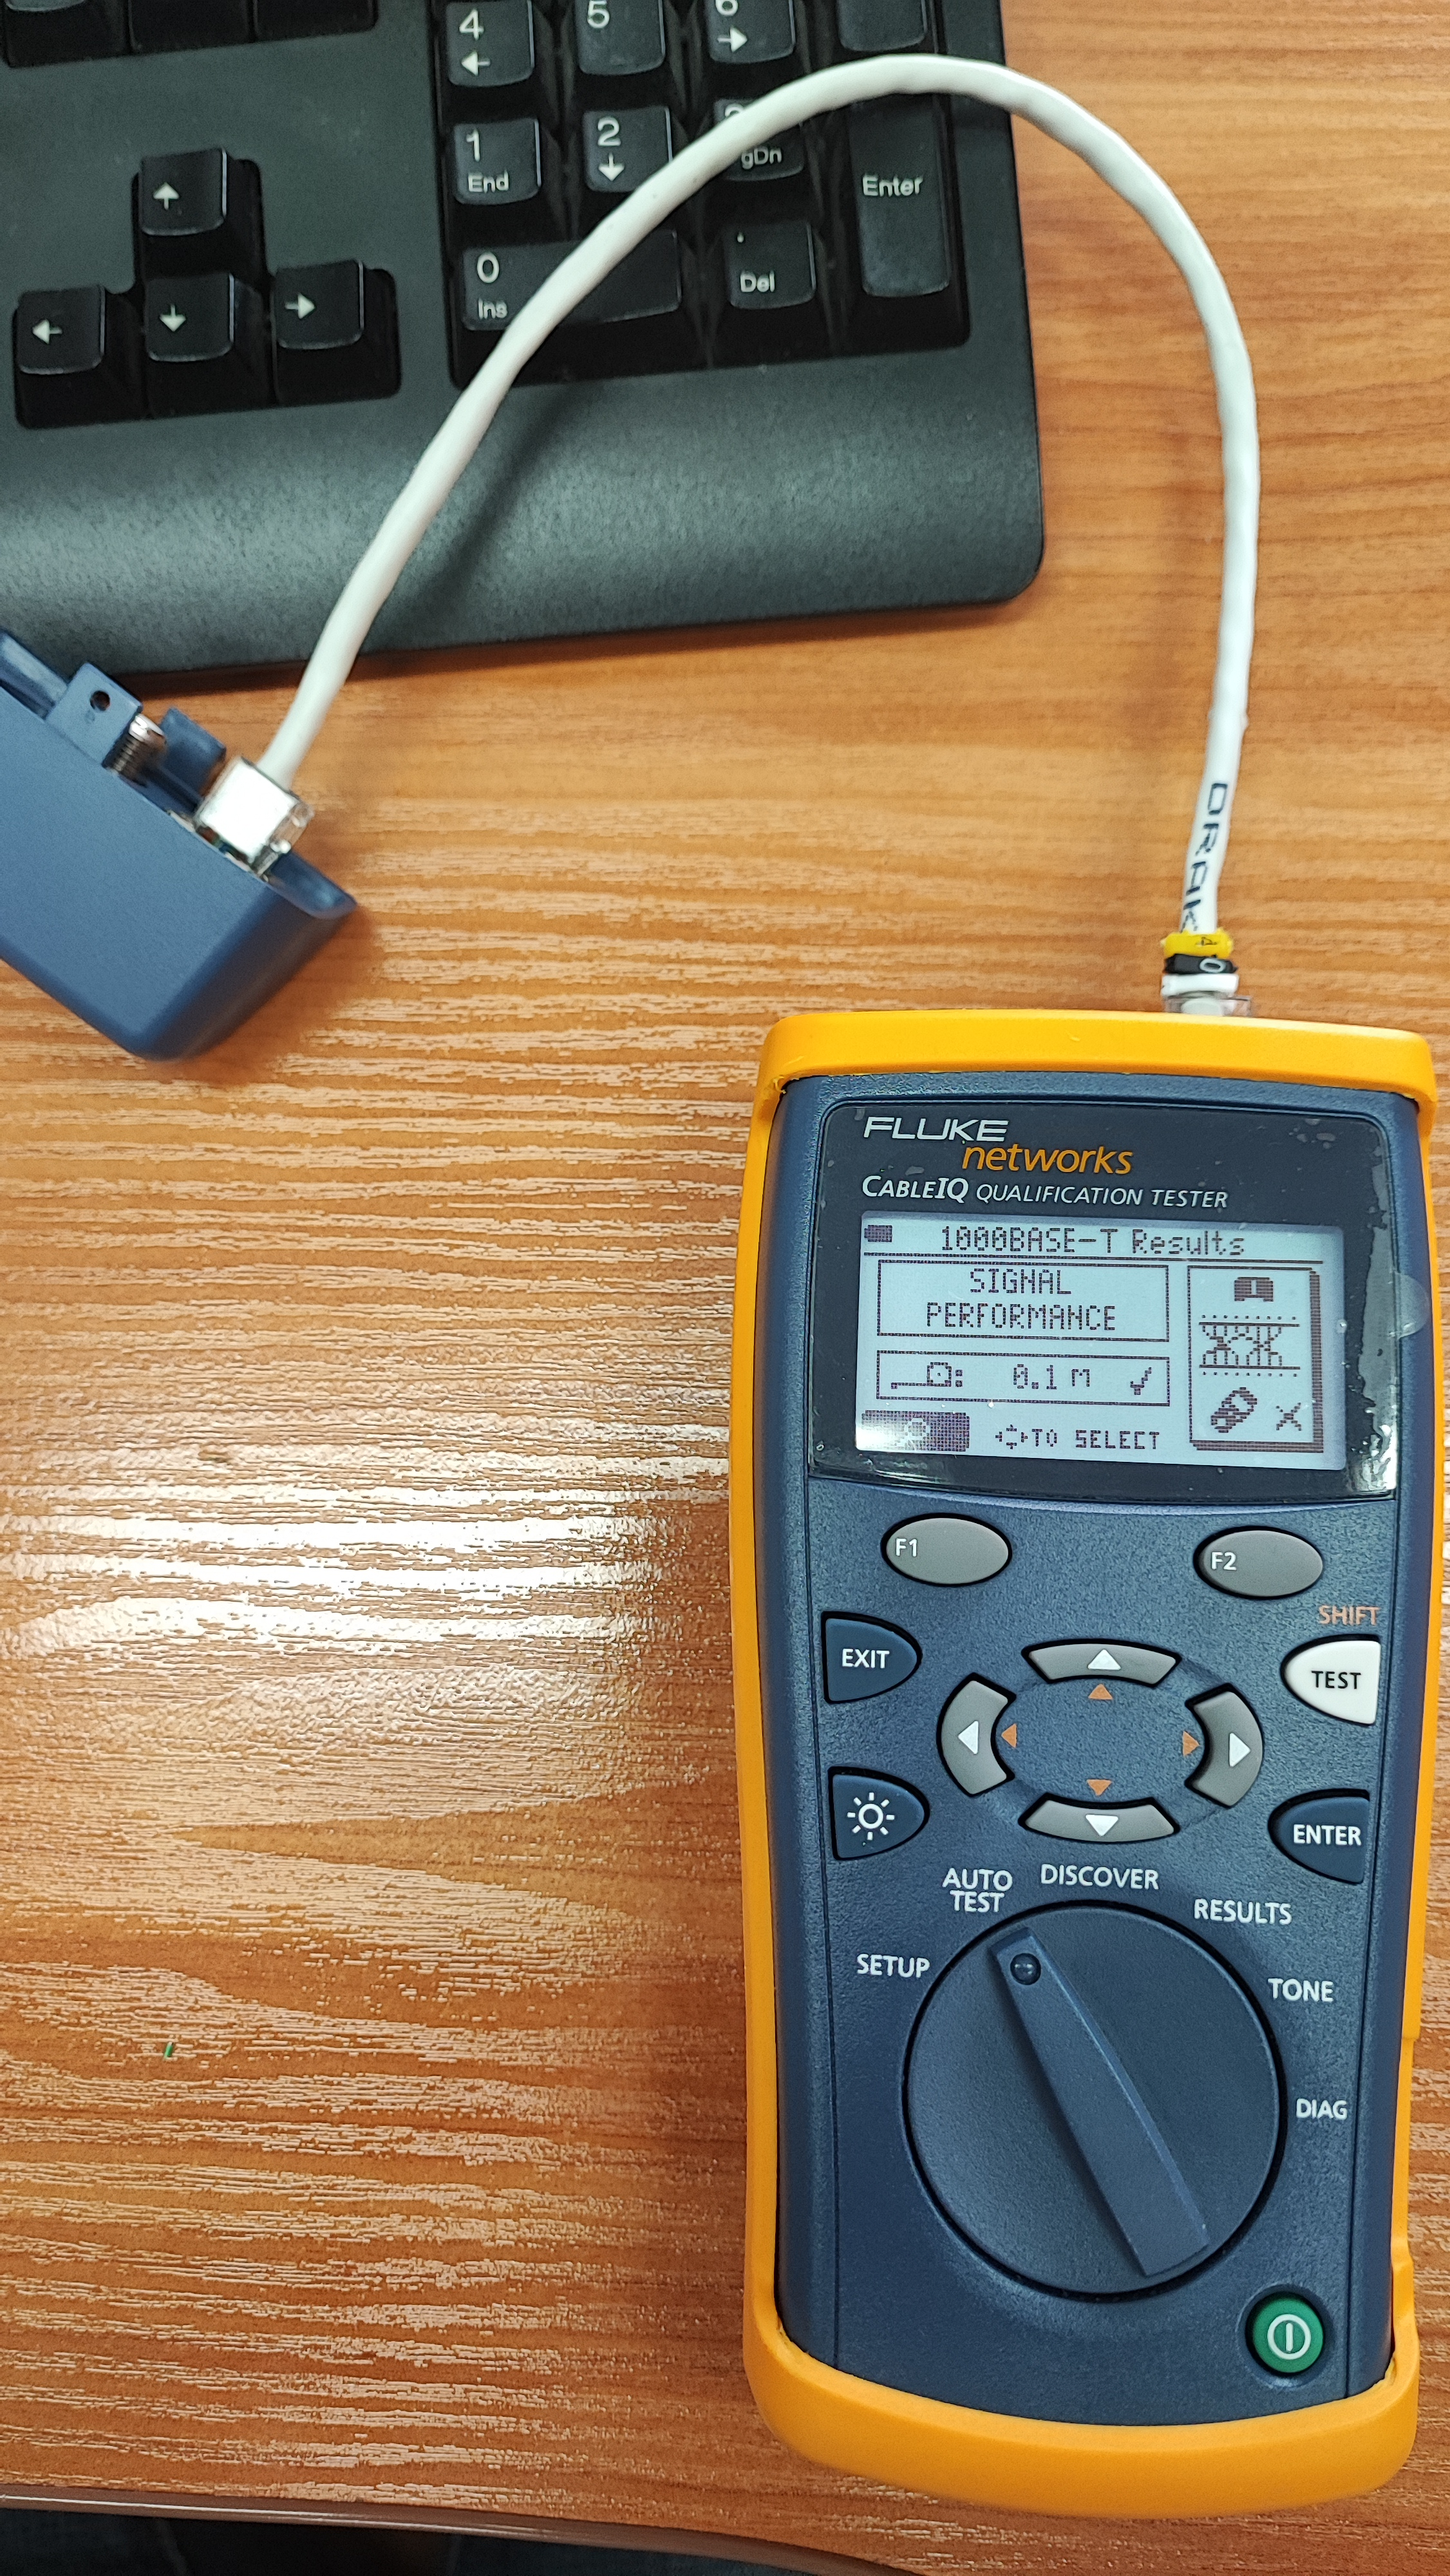
\includegraphics[height=0.31\textheight]{fluke_wiring_fault_hot_tested.jpg}
\caption{Seria zdjęć 124458 i 124507: pomiary z wykrytą usterką}
\end{minipage}\hfill
\begin{minipage}{0.48\textwidth}
\centering
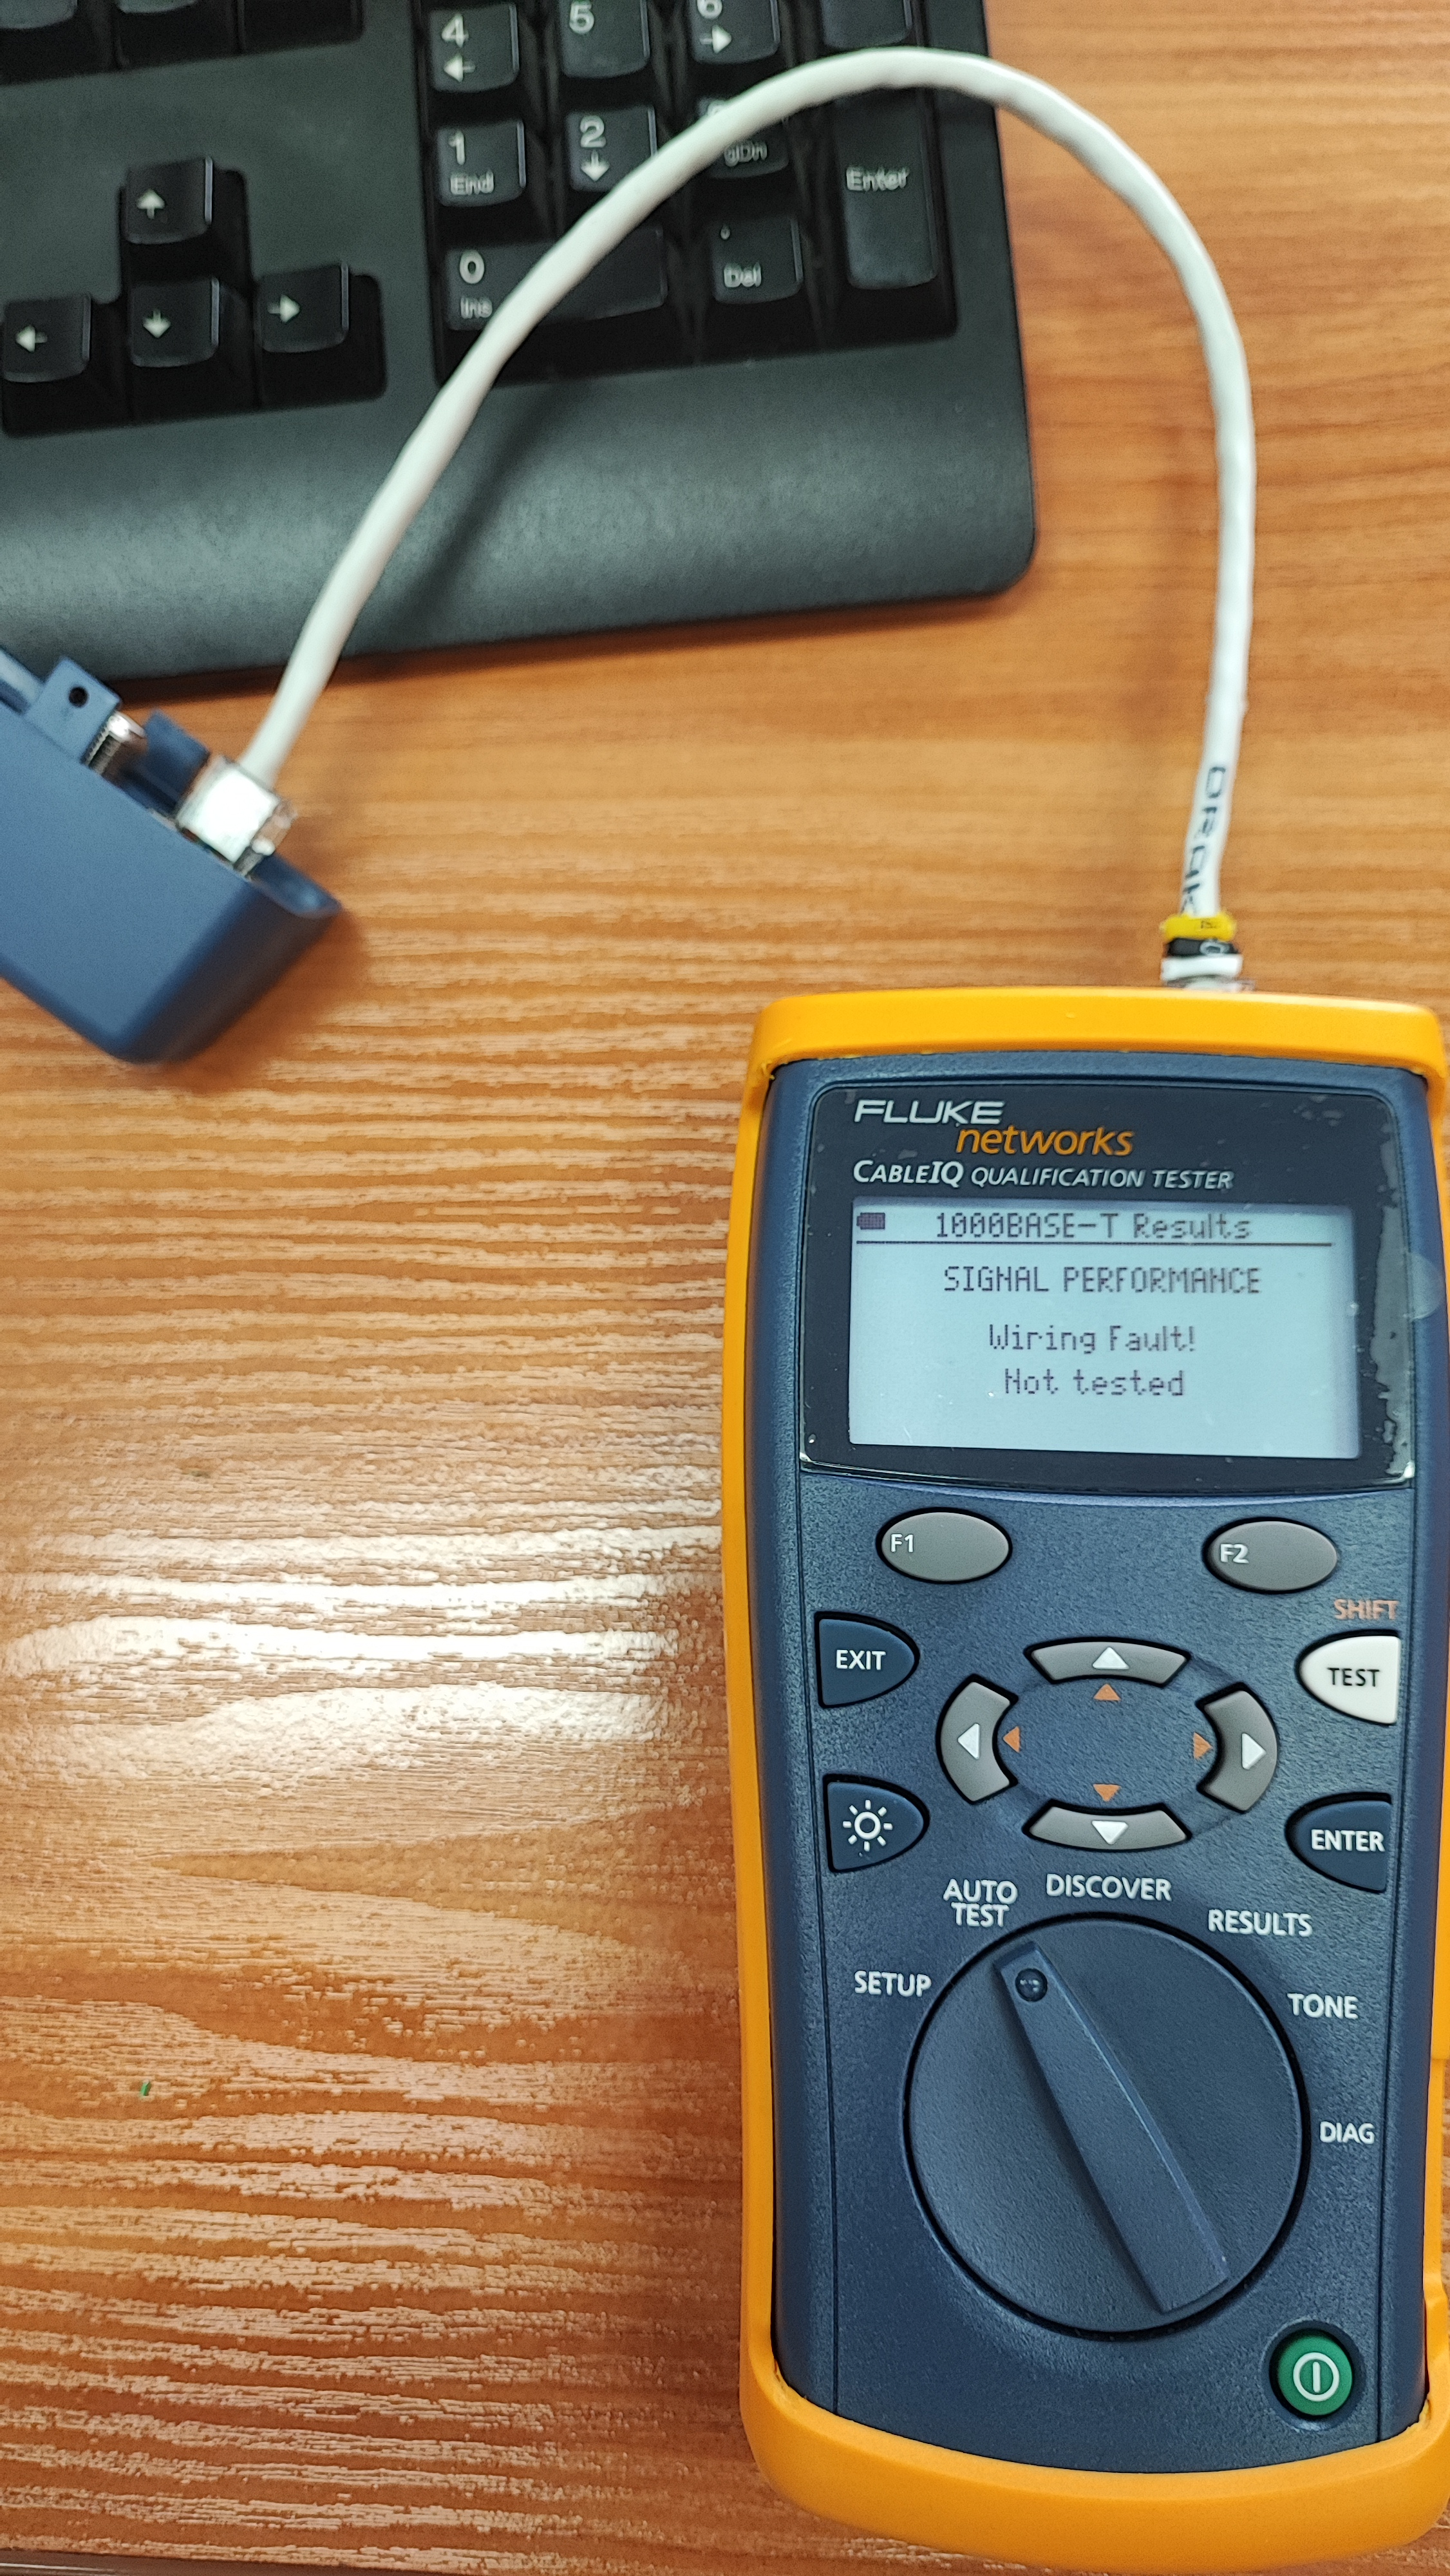
\includegraphics[height=0.31\textheight]{fluke_wiring_fault_hot_tested_second.jpg}
\caption{Seria zdjęć 124458 i 124507: pomiary z wykrytą usterką}
\end{minipage}
\end{figure}

\begin{figure}[H]
\centering
\begin{minipage}{0.48\textwidth}
\centering
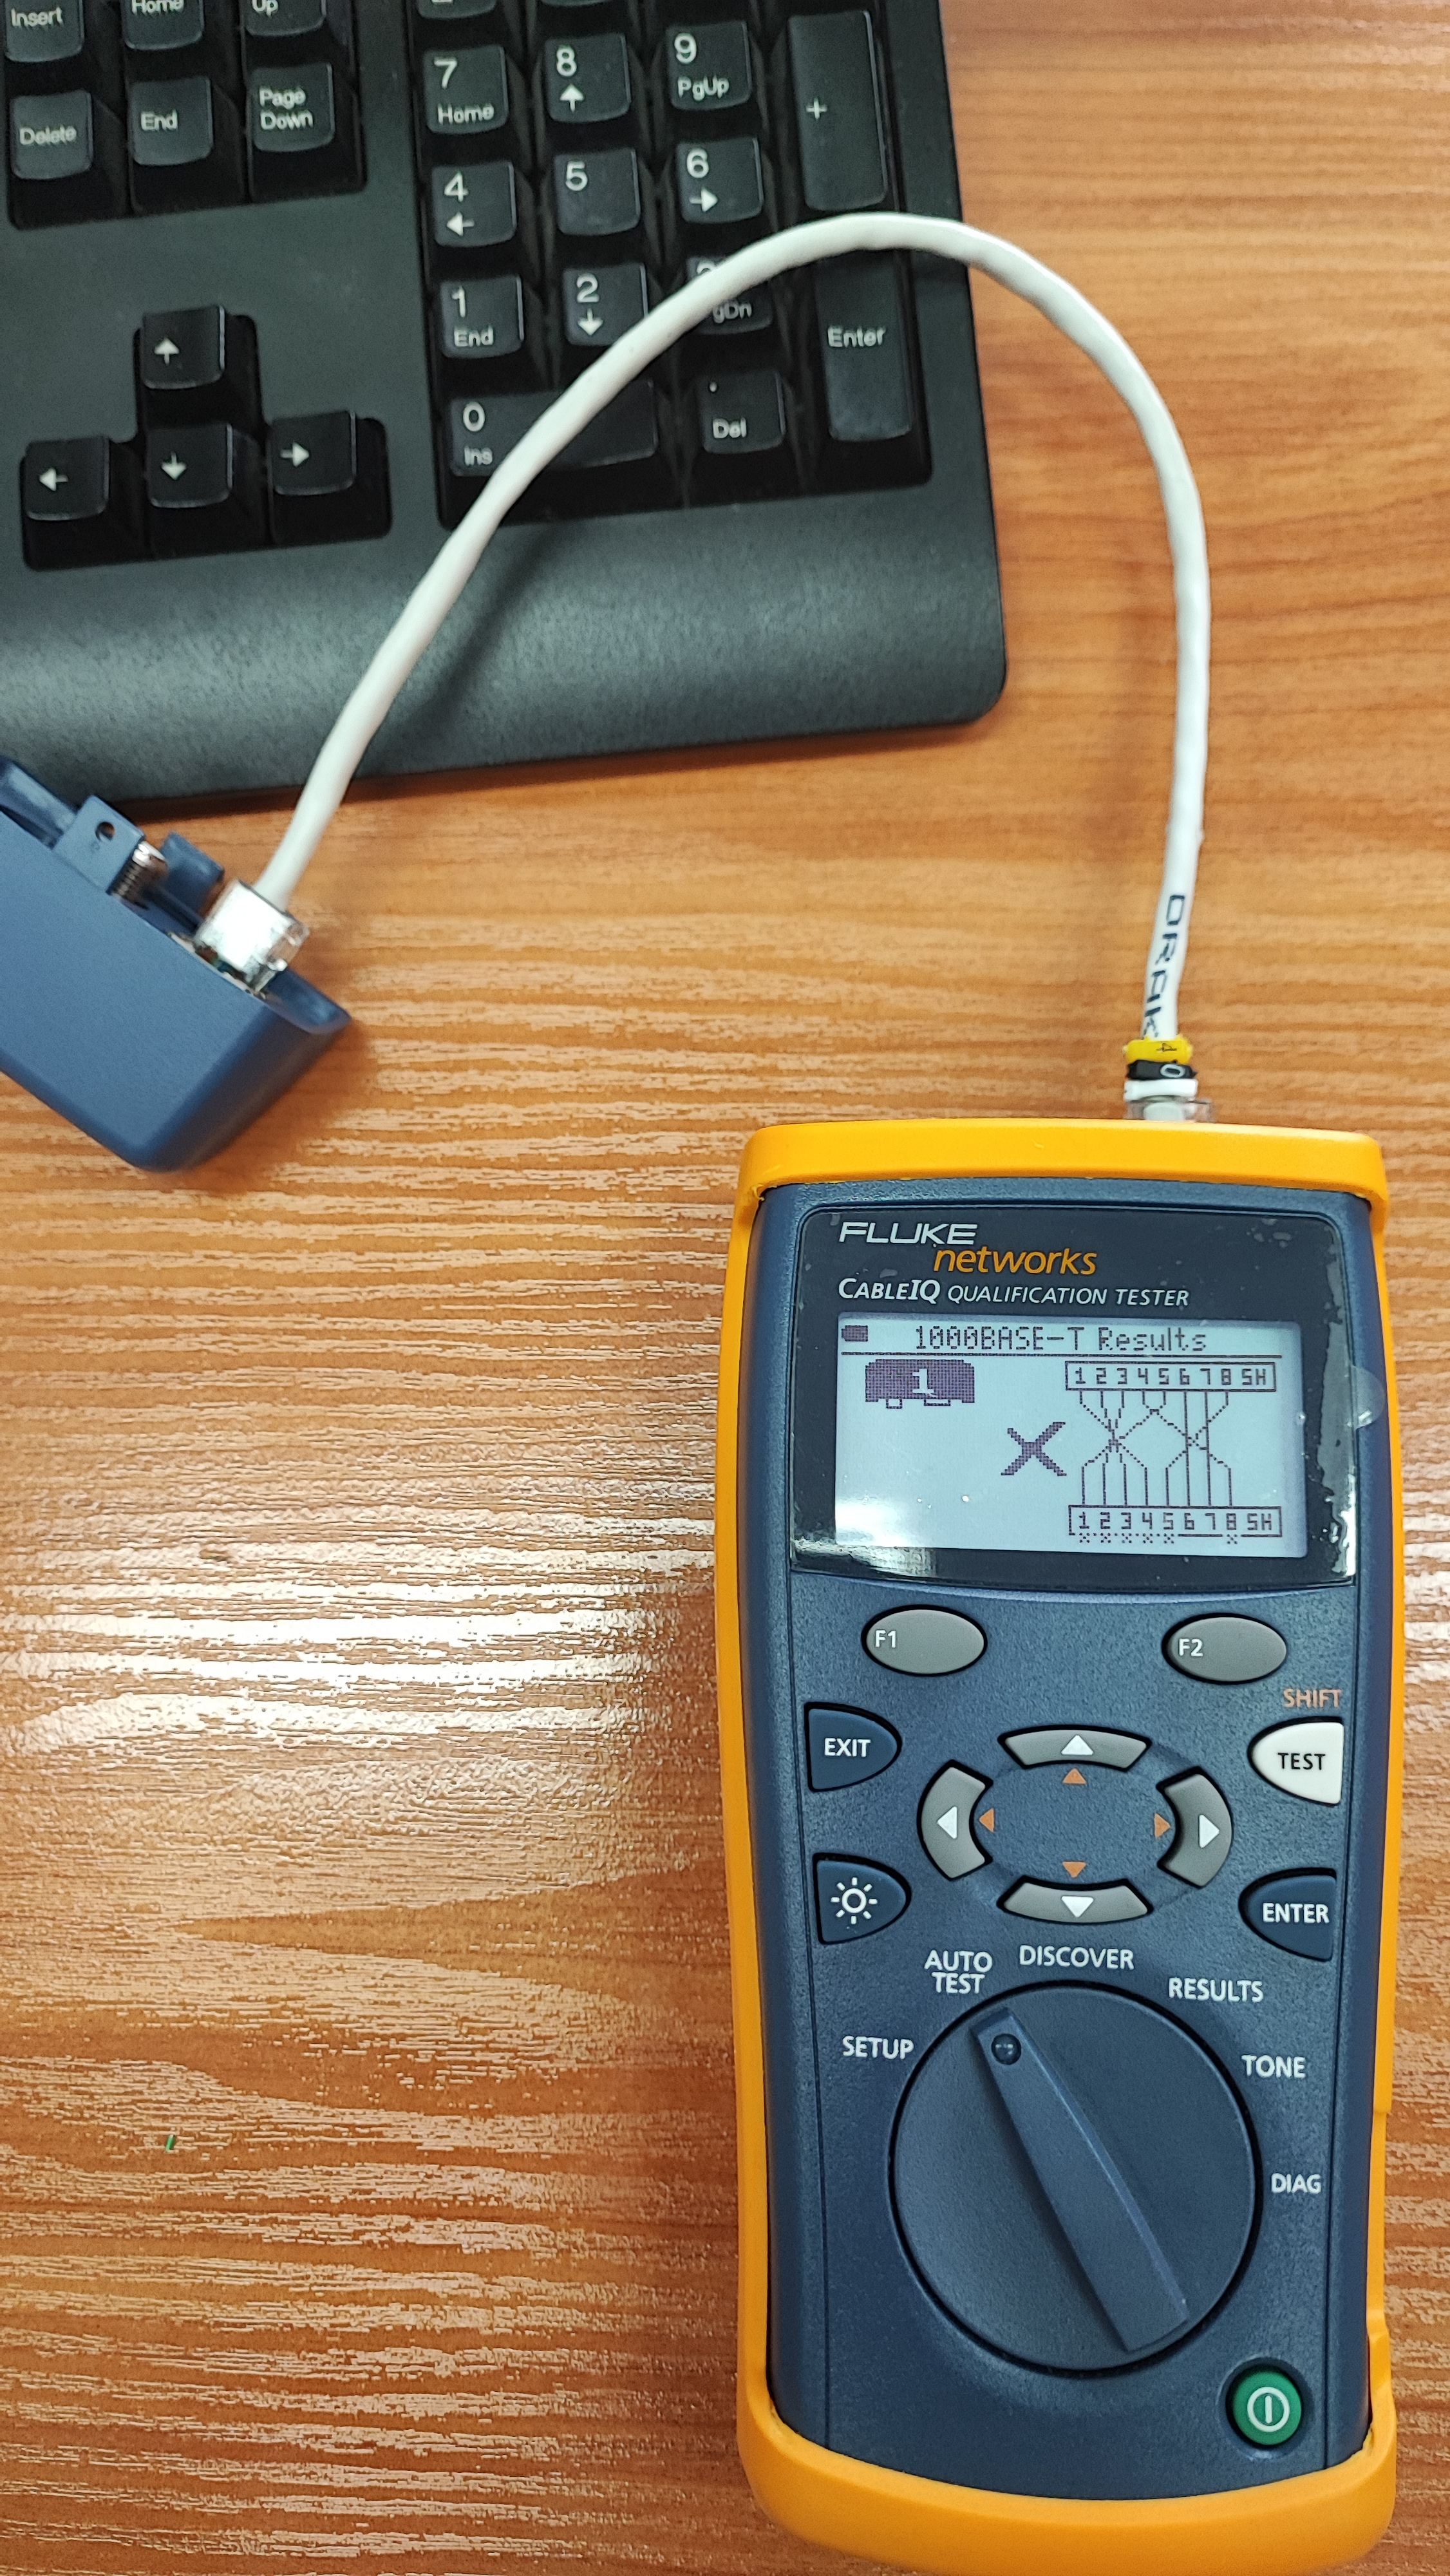
\includegraphics[height=0.31\textheight]{fluke_wiring_fault_hot_tested_third.jpg}
\caption{Seria zdjęć 124516 i 124523: kolejne wyniki testów z usterkami}
\end{minipage}\hfill
\begin{minipage}{0.48\textwidth}
\centering
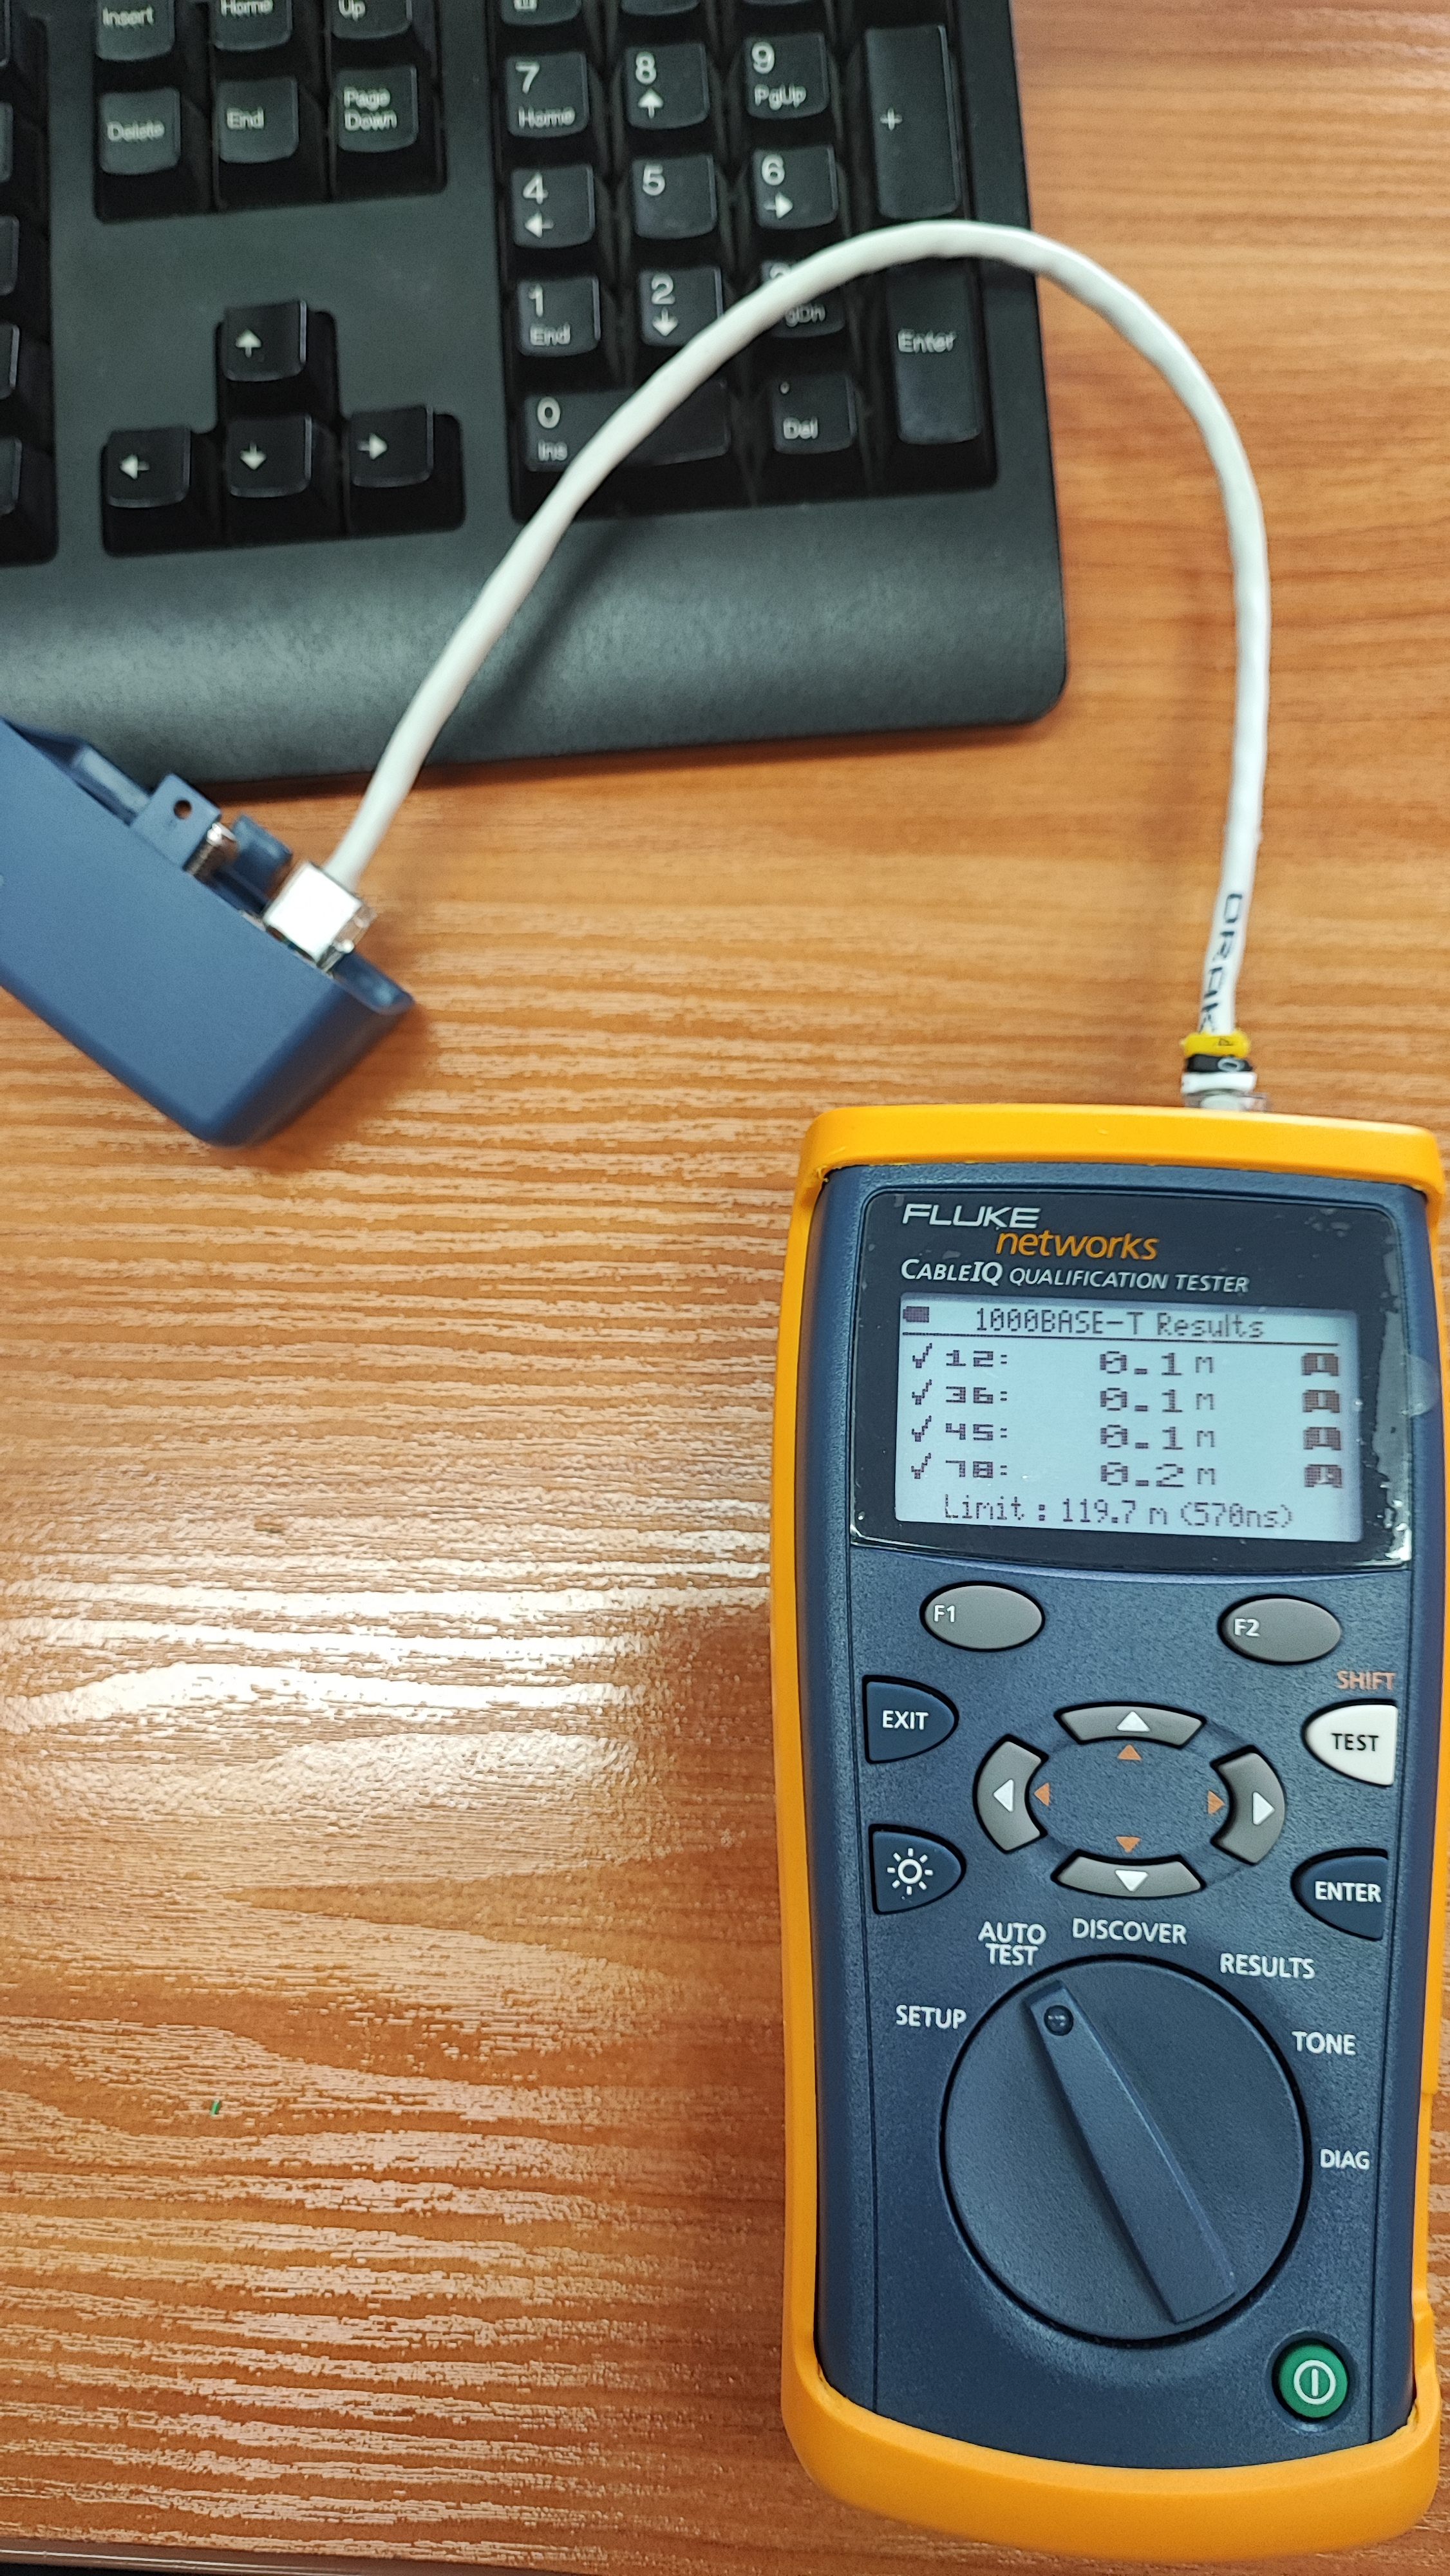
\includegraphics[height=0.31\textheight]{fluke_wiremap_crossover.jpg}
\caption{Seria zdjęć 124516 i 124523: kolejne wyniki testów z usterkami}
\end{minipage}
\end{figure}

\begin{figure}[H]
\centering
\begin{minipage}{0.48\textwidth}
\centering
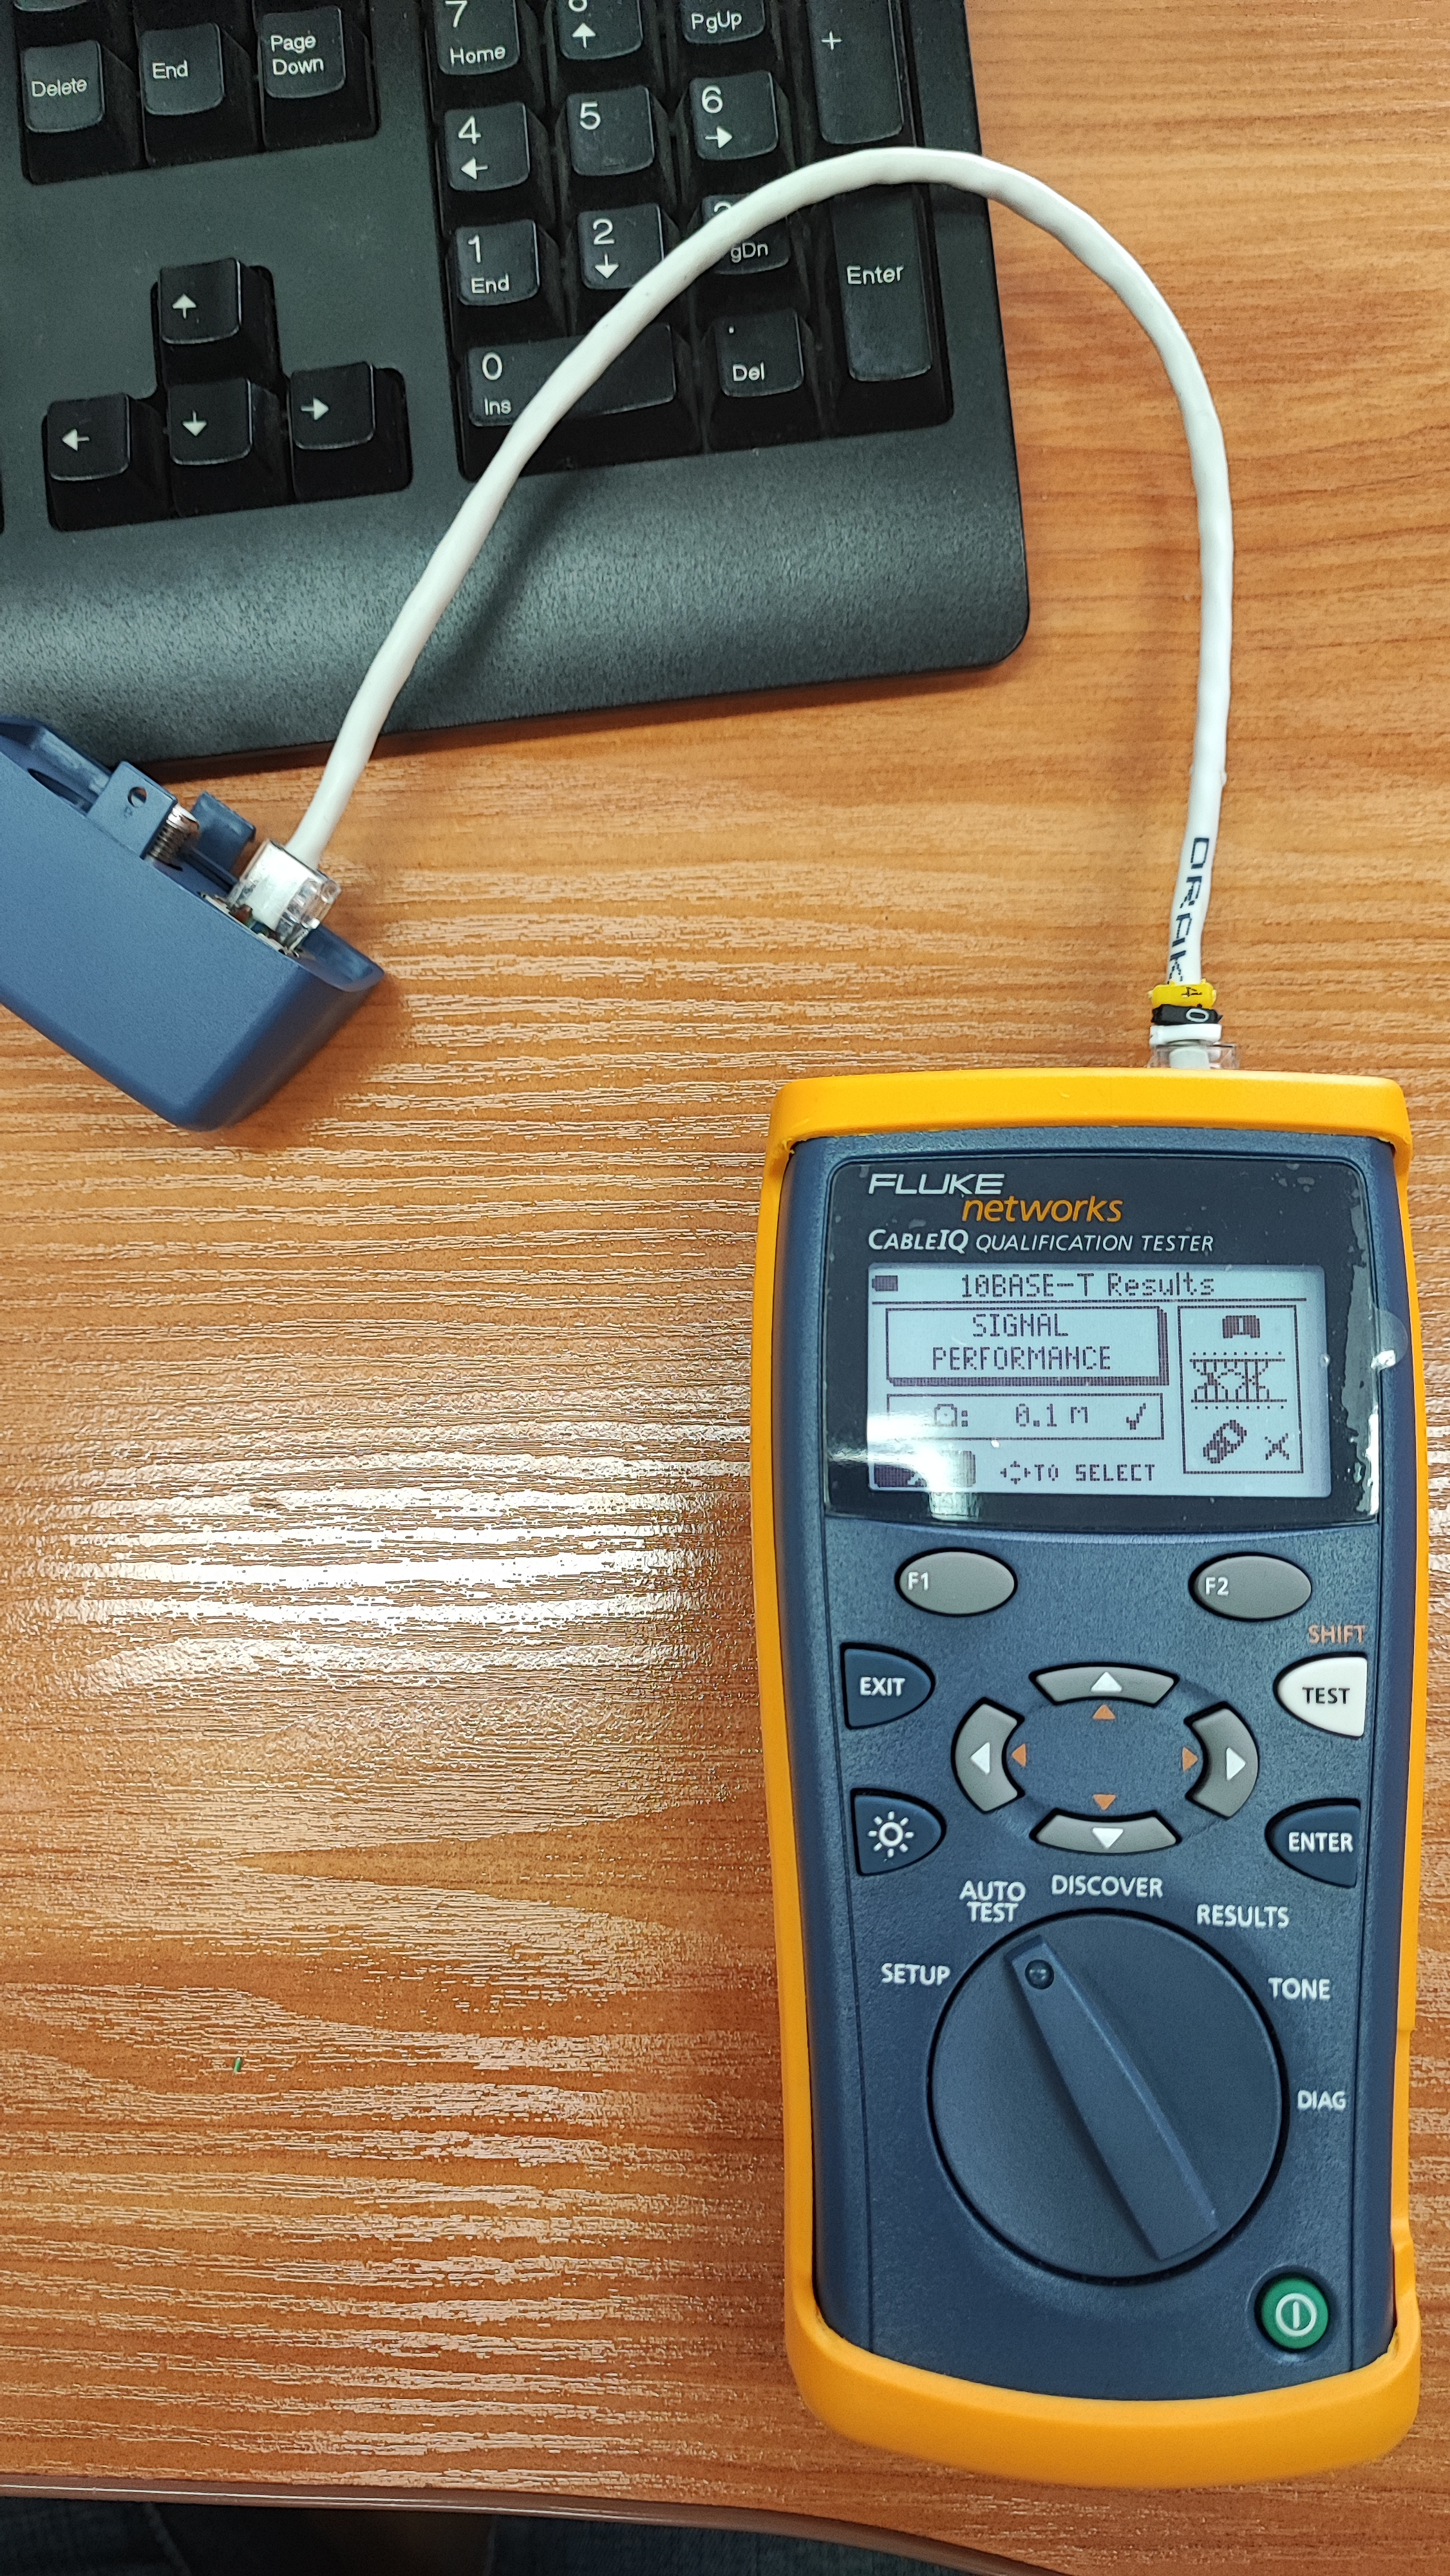
\includegraphics[height=0.31\textheight]{fluke_wiremap_crossover_second.jpg}
\caption{Seria zdjęć 124530 i 124538: mapy połączeń z usterkami}
\end{minipage}\hfill
\begin{minipage}{0.48\textwidth}
\centering
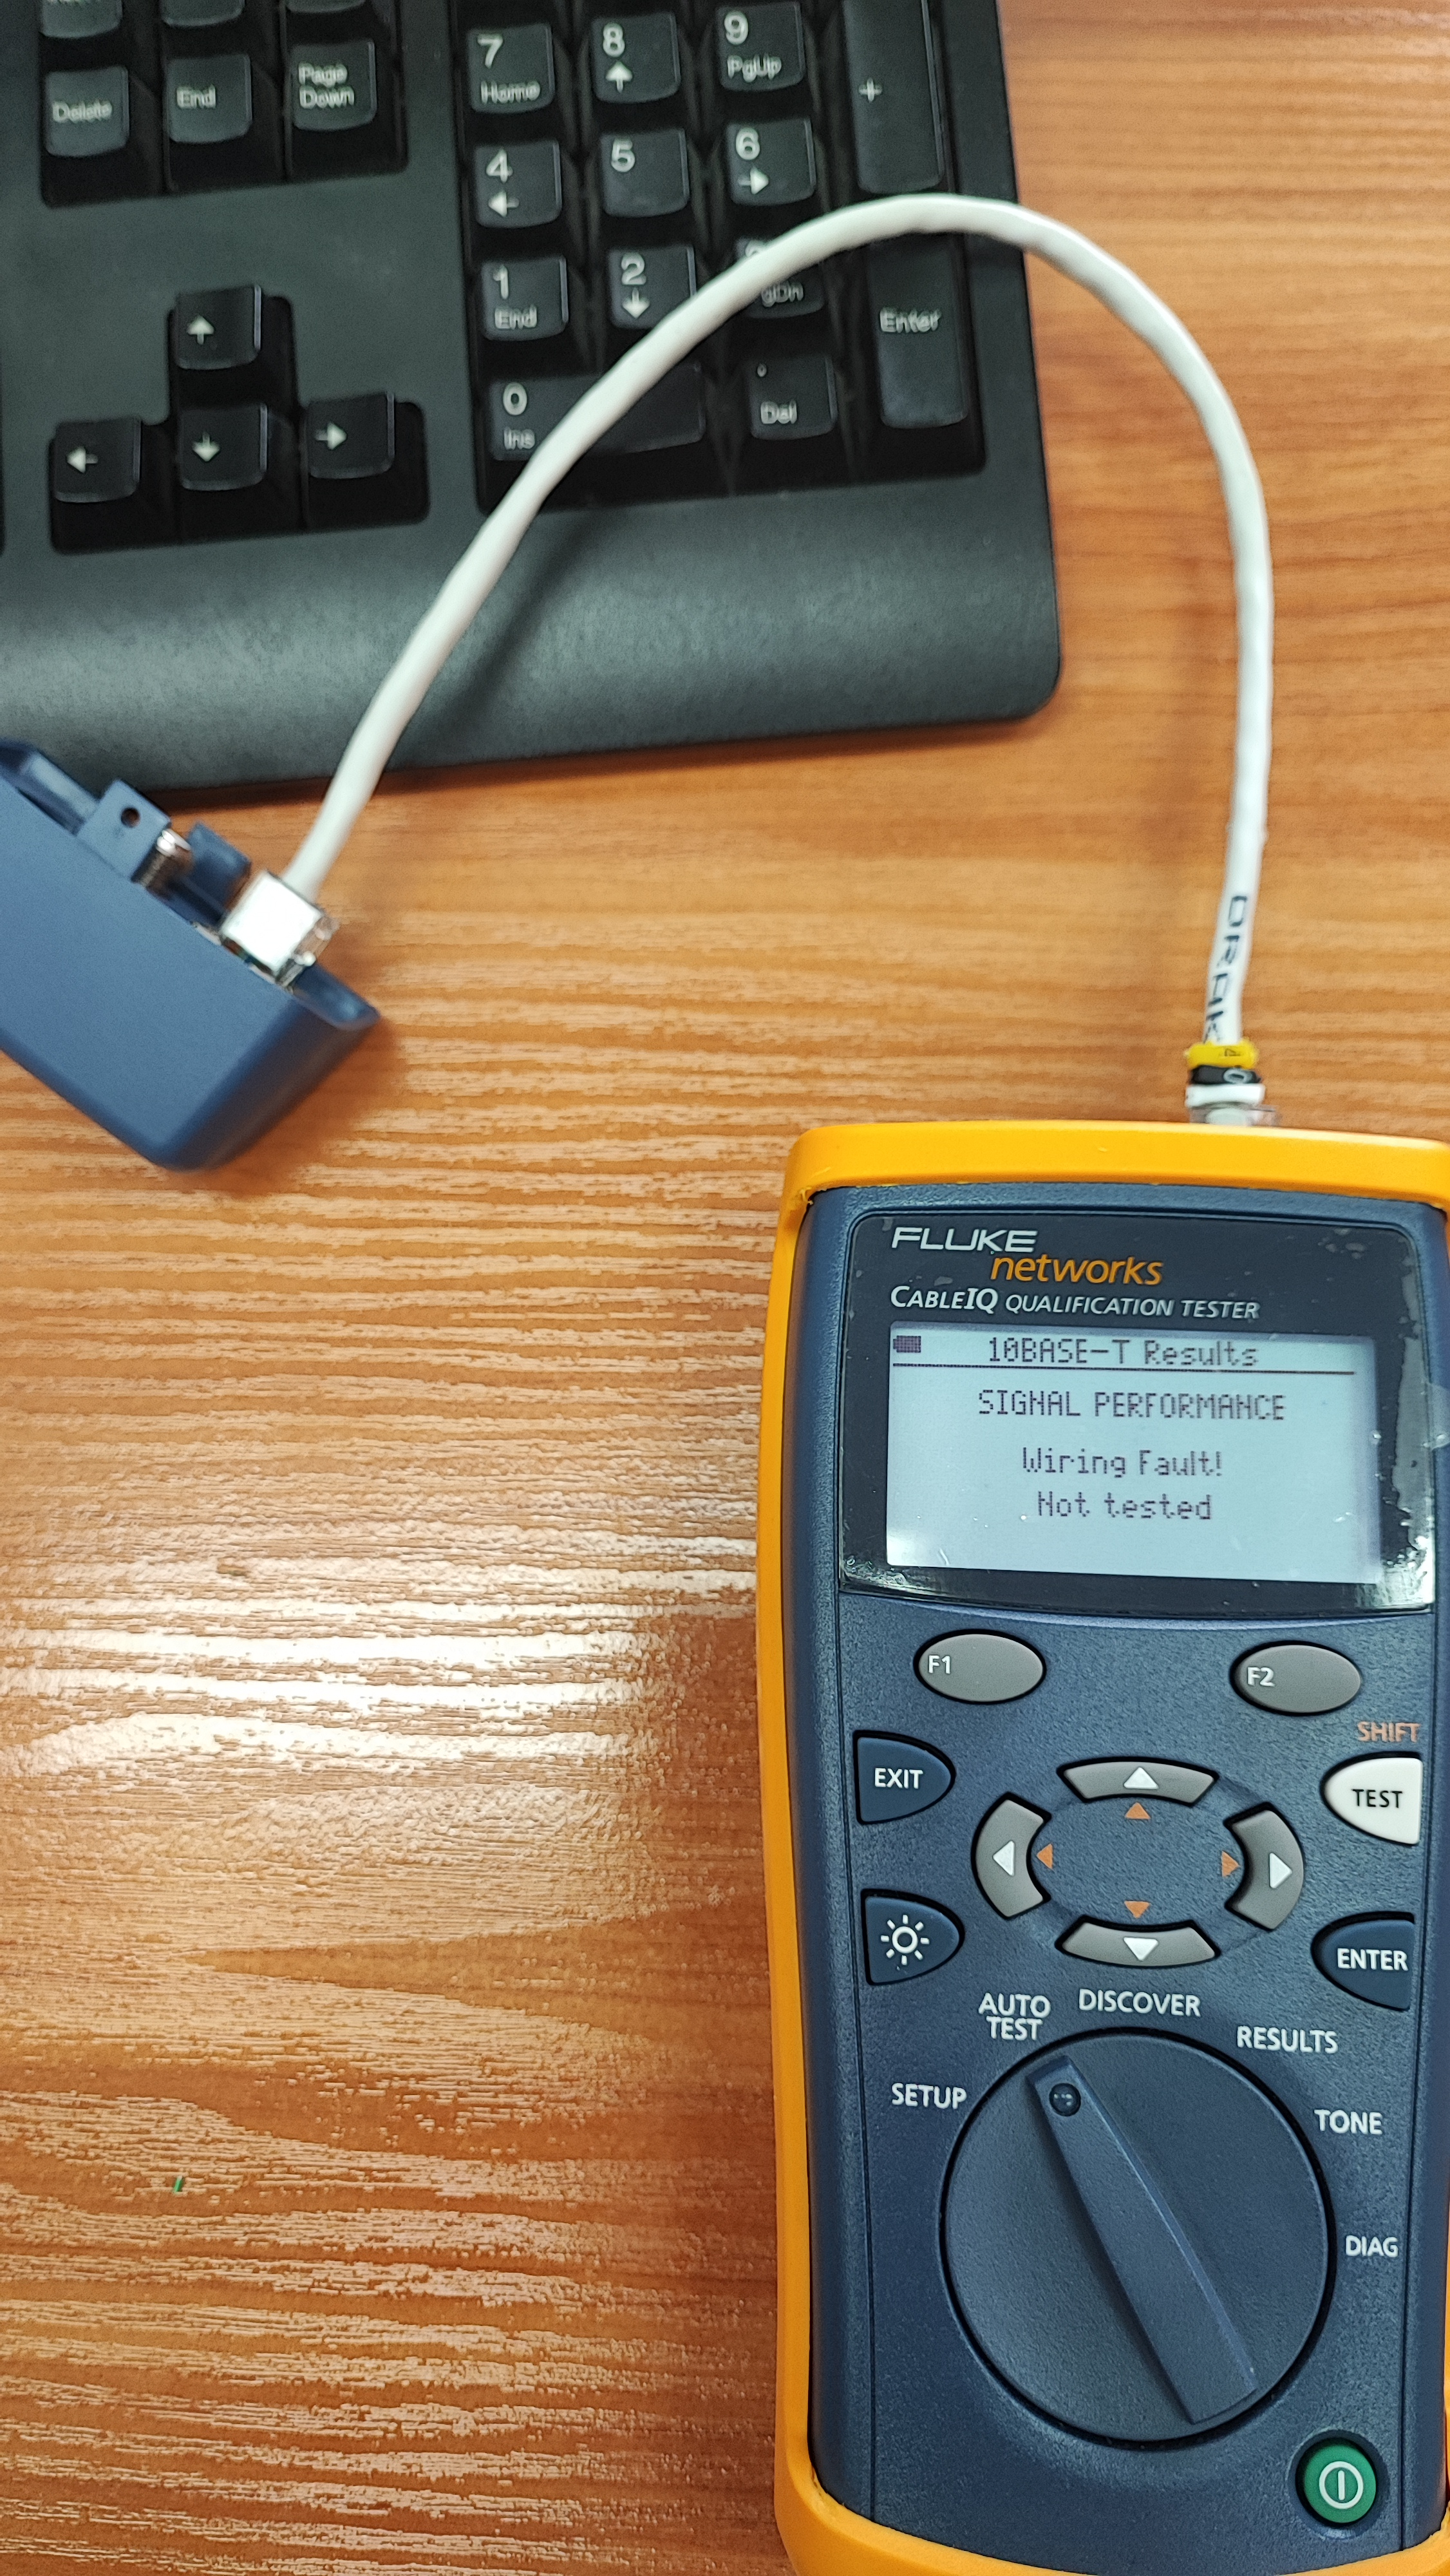
\includegraphics[height=0.31\textheight]{fluke_wiring_fault_map.jpg}
\caption{Seria zdjęć 124530 i 124538: mapy połączeń z usterkami}
\end{minipage}
\end{figure}

\subsection{Pozostałe zdjęcia i schematy ręczne}
Oprócz zdjęć numerowanych galeria obejmuje następujące pliki:
\begin{itemize}
  \item \texttt{notes\_cables\_62\_40\_60.jpg} -- schematy połączeń i długości kabli,
  \item \texttt{notes\_cable\_numbers\_lengths.jpg} -- numery kabli i ręczne zestawienia,
  \item \texttt{lab\_scenario\_and\_connection\_drawing.jpg} -- scenariusz i propozycja ścieżki,
  \item \texttt{rj45\_prepared\_connector.jpg}, \texttt{rj45\_connector\_from\_wire\_side.jpg}, \texttt{patchcord\_rj45\_control.jpg} i \texttt{patchcord\_finished\_connector.jpg} -- wykonanie i kontrola wtyczek oraz patchcordów.
\end{itemize}

\subsection{Nagrania}
Zanalizowaliśmy i udokumentowaliśmy wszystkie pliki .mp4. Ich reprezentatywne klatki znajdują się w rozdziale \emph{Dokumentacja filmów}.
\end{document}
